\documentclass[letterpaper,10pt]{book}
% Change to 10 pt
\usepackage{pdfpages}
\usepackage{morewrites}			% to counteract the no write space problem
\setcounter{tocdepth}{6}

\usepackage[framemethod=TikZ]{mdframed}

\usepackage{fancyhdr}

\usepackage{paralist}
\usepackage{amsmath}
\usepackage{amsfonts}
\usepackage{amssymb}
\usepackage{graphicx}

\usepackage{datetime}
%\usepackage{ulem}

%\usepackage[nottoc]{toobibind}

\usepackage[inline]{enumitem}

% Outer margin at 2.50 is exacty correct to fit the ``corruption alert'' tables
\usepackage[inner=1.0in, outer=2.50in, top=2.54cm,bottom=2.54cm, marginparwidth=2.25in]{geometry}

\usepackage{marginnote}
\usepackage{longtable}
\usepackage{booktabs}
\usepackage{xcolor}

\usepackage{soul}

%%%%%%%%%%%%
\definecolor{ForestGreen}{rgb}{0.00,0.29,0.098}
%%%%%%%%%%%%

\usepackage{marginnote}

\usepackage{imakeidx} 
\usepackage[
	backref=true,
	style=numeric,
%	citestyle=numeric,
	backend=bibtex
	]{biblatex}
\usepackage[driverfallback=hypertex,colorlinks=True]{hyperref}
\usepackage{cleveref}

\makeindex[name=scripture,columnsep=20pt, columnseprule=True,columns=3, title=Scripture References]
\makeindex[name=speaker,columnsep=20pt, columnseprule=True,,columns=2, title=Sermon Creator]
\makeindex[name=series,columnsep=20pt, columnseprule=True,,columns=2, title=Sermon Series]
\makeindex[name=date,columnsep=20pt, columnseprule=True,columns=2, title=Sermon Date]
\makeindex[name=event,columnsep=20pt, columnseprule=True,columns=2, title=Event]
\makeindex[name=topic,columnsep=20pt, columnseprule=True,columns=2, title=Topic]
\makeindex[name=AWIP,columnsep=20pt, columnseprule=True,columns=3, title=All Words in Passage]
\makeindex[name=NWIV,columnsep=20pt, columnseprule=True,columns=3, title=Number of Words in Verse]
\makeindex[name=PNIP,columnsep=20pt, columnseprule=True,columns=3, title=Proper Names in Passage]
\makeindex[name=PEIP,columnsep=20pt, columnseprule=True,columns=2, title=Prophetic Events in Passage]
\makeindex[name=TWPAQ,columnsep=20pt, columnseprule=True,columns=1, title=13-Word Phrases and Quotes]
\makeindex[name=PFTTIS,columnsep=20pt, columnseprule=False,columns=3, title=Phrases found 13 times in scripture]
\makeindex[name=WFTTIS,columnsep=20pt, columnseprule=False,columns=3, title=Words found 13 times in scripture]
\makeindex[name=WFITV,columnsep=20pt, columnseprule=False,columns=3, title=Words found in exactly 13 verses]
\makeindex[name=EVENTS,columnsep=20pt, columnseprule=False,columns=2, title=Sermon Log by Place]
\makeindex[name=QUESTIONS,columnsep=20pt, columnseprule=False,columns=2, title=Bible Questions]
\makeindex[name=DOCTRINES,columnsep=20pt, columnseprule=False,columns=2, title=Doctrines]
\makeindex[name=SONGS,columnsep=20pt, columnseprule=False,columns=1, title=Songs]
\makeindex[name=LOCATION,columnsep=20pt, columnseprule=False,columns= 2, title=Location]
\makeindex[name=FACEBOOK,columnsep=20pt, columnseprule=False,columns=2, title=Facebook]
\makeindex[name=DEVOTIONAL,columnsep=20pt, columnseprule=False,columns=2, title=Devotional Items]
%%%%%%%%%%%%%%%%% EXTRA COLORS
\definecolor{champagne}{rgb}{0.97,0.91,0.81}
\definecolor{bone}{rgb}{0.89,0.85,0.79}
\pagestyle{fancy}
\fancyhf{}
\fancyhead[LE,RO]{\today}
\fancyhead[RE,LO]{Daily Bible Reading}
\fancyhead[CE,CO]{-page \thepage  - }

\fancyfoot[CO,CE]{\leftmark}
%\fancyfoot[LE,RO]{CSCE 692, HW1}

\title{DBR\\
Daily \\ Reads}
\author{Keith Anthony \\
\today }
%+/ffffff +   \pagenumbering{gobble}
\bibliography{Bibliographies/All20220122}

\setlength{\fboxsep}{1.0pt}

\usepackage[utf8]{inputenc}
\usepackage{tikz}

\begin{document}
%%%%%%%%%%%% Tile Page

\begin{titlepage}

\begin{flushright}
\rightskip=-2.5cm
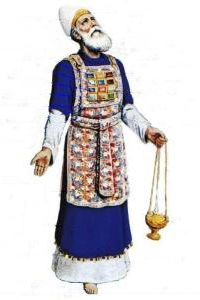
\includegraphics[width=50mm,scale=1.5]{Extras/Melchisedec.jpg}
\vspace{0.4in}  % Create a title for the document and write it in bold font
\LARGE{\textbf{\date}} % Again, do a line break
\linebreak 
% Create a subtitle \large{with Outlines, Statistics, Cross References, and Notes}
\vspace{0.5in}
\begin{flushleft}
\LARGE{Day \#57: Saturday, 26 February 2022 LITE  \\}\vspace{0.25in}
\LARGE{Deuteronomy 13-15 Psalm 57 Proverb 26}
\end{flushleft}
\vspace{0.6in}
\bigskip

\normalsize{Xenia, Oh.\\}
\normalsize{created: \today}
\vspace{1.3in}

\end{flushright}
\end{titlepage}

\newpage 
\tableofcontents\hypertarget{TOC}{}
\listoffigures
\listoftables

\hyphenation{A-bim-e-lech bre-thren E-phra-im  Gib-e-o-nites Jer-u-sa-lem through-out Phil-i-stines The-o-phil-us Am-a-le-kites ven-geance Mesh-el-e-mi-ah onan-ism Phar-a-oh thoughts grev-ous-ness Hach-a-liah adul-ter-er Shad-rach}

%%%%%%%%%%%%%%%%% EXTRA COLORS
%%%%%%%%%%%%%%%%% EXTRA COLORS
%%%%%%%%%%%%%%%%% EXTRA COLORS
\definecolor{champagne}{rgb}{0.97,0.91,0.81}
\definecolor{bone}{rgb}{0.89,0.85,0.79}

\definecolor{ForestGreen}{rgb}{0.00,0.29,0.098}
\definecolor{GIVING}{cmyk}{1,0.0,0.72,.1}

\definecolor{MLPE}{cmyk}{1,1,0,.45}
\definecolor{SOCCER}{cmyk}{.77, 0, .42, .49}
\definecolor{PAYBILL}{cmyk}{0,0.83,0.76,0.07}
\definecolor{SERMON}{cmyk}{.14,.9,0,.30} % aka seance \href{http://www.flatuicolorpicker.com/purple-cmyk-color-model/}{seance}
\definecolor{BIBLE}{cmyk}{0,.17,.74,.17}
\definecolor{WORKBLUE}{cmyk}{1, .5, 0, .6}
\definecolor{myOrange}{cmyk}{0, .4, .98, .03}
\definecolor{myTan}{cmyk}{0.0,.07,.17,.10}
\definecolor{myRed}{cmyk}{0,1,1,0}
\definecolor{myWhite}{cmyk}{0,0,0,0}
\definecolor{BLUESoD}{cmyk}{.97,.84,0,.04}
\definecolor{WHITE}{cmyk}{0,0,0,0}
\definecolor{OLDGOLD}{cmyk}{0.05,0.3,1.00,0}
\definecolor{CASTLETON}{cmyk}{1,0,0.31,0.66}
\definecolor{cadmiumgreen}{rgb}{0.0, 0.42, 0.24}
\definecolor{jungle}{rgb}{0.203,0.4882,0.1718}
\definecolor{MYGOLD}{rgb}{1,.84,0}

\definecolor{MYLIGHTGRAY}{rgb}{.85,.85,.85}

\definecolor{codegreen}{rgb}{0,0.6,0}
\definecolor{codegray}{rgb}{0.5,0.5,0.5}
\definecolor{codepurple}{rgb}{0.58,0,0.82}
\definecolor{backcolour}{rgb}{0.95,0.95,0.92}


\mdfdefinestyle{MyFrame}{%
    linecolor=blue,
    outerlinewidth=2pt,
    roundcorner=5pt,
    innertopmargin=\baselineskip,
    innerbottommargin=\baselineskip,
    innerrightmargin=10pt,
    innerleftmargin=10pt,
    backgroundcolor=gray!25!white}


\mdfdefinestyle{MyFrame2}{%
    linecolor=black,
    outerlinewidth=2pt,
    roundcorner=5pt,
    innertopmargin=\baselineskip,
    innerbottommargin=\baselineskip,
    innerrightmargin=10pt,
    innerleftmargin=10pt,
    backgroundcolor=yellow!25!white}


%%%%%
%% for PFTTIS list
%%%%%

%%% And Joseph said unto
\index[PFTTIS]{And Joseph said unto!Genesis!Gen 40:008}
\index[PFTTIS]{And Joseph said unto!Genesis!Gen 40:012}
\index[PFTTIS]{And Joseph said unto!Genesis!Gen 41:025}
\index[PFTTIS]{And Joseph said unto!Genesis!Gen 42:014}
\index[PFTTIS]{And Joseph said unto!Genesis!Gen 42:018}
\index[PFTTIS]{And Joseph said unto!Genesis!Gen 44:015}
\index[PFTTIS]{And Joseph said unto!Genesis!Gen 45:003}
\index[PFTTIS]{And Joseph said unto!Genesis!Gen 45:004}
\index[PFTTIS]{And Joseph said unto!Genesis!Gen 46:031}
\index[PFTTIS]{And Joseph said unto!Genesis!Gen 48:009}
\index[PFTTIS]{And Joseph said unto!Genesis!Gen 48:018}
\index[PFTTIS]{And Joseph said unto!Genesis!Gen 50:019}
\index[PFTTIS]{And Joseph said unto!Genesis!Gen 50:024}


%%% a shadow
\index[PFTTIS]{a shadow!1Chronicles!1Chr 029:15}
\index[PFTTIS]{a shadow!Job!Job 008:09}
\index[PFTTIS]{a shadow!Job!Job 014:02}
\index[PFTTIS]{a shadow!Job!Job 017:07}
\index[PFTTIS]{a shadow!Psalm!Psa 102:011}
\index[PFTTIS]{a shadow!Psalm!Psa 144:004}
\index[PFTTIS]{a shadow!Ecclesiastes!Eccl 006:012}
\index[PFTTIS]{a shadow!Ecclesiastes!Eccl 008:013}
\index[PFTTIS]{a shadow!Isaiah!Isa 04:006}
\index[PFTTIS]{a shadow!Isaiah!Isa 25:004}
\index[PFTTIS]{a shadow!Jonah!Jnh 04:06}
\index[PFTTIS]{a shadow!Colossians!Col 02:017}
\index[PFTTIS]{a shadow!Hebews!Heb 10:001}

%%% blessed is the man
\index[PFTTIS]{blessed is the man!Psalm!Psa 001:001}
\index[PFTTIS]{blessed is the man!Psalm!Psa 032:002}
\index[PFTTIS]{blessed is the man!Psalm!Psa 034:008}
\index[PFTTIS]{blessed is the man!Psalm!Psa 065:004}
\index[PFTTIS]{blessed is the man!Psalm!Psa 084:005}
\index[PFTTIS]{blessed is the man!Psalm!Psa 084:012}
\index[PFTTIS]{blessed is the man!Psalm!Psa 094:012}
\index[PFTTIS]{blessed is the man!Psalm!Psa 112:001}
\index[PFTTIS]{blessed is the man!Proverbs!Pro 008:034}
\index[PFTTIS]{blessed is the man!Isaiah!Isa 056:002}
\index[PFTTIS]{blessed is the man!Jeremiah!Jer 017:007}
\index[PFTTIS]{blessed is the man!Romans!Rom 004:008}
\index[PFTTIS]{blessed is the man!James!Jam 001:012}


%%% carry them
\index[PFTTIS]{carry them!Leviticus!Lev 14:045}
\index[PFTTIS]{carry them!Numbers!Num 11:012}
\index[PFTTIS]{carry them!Joshua!Jsh 04:003}
\index[PFTTIS]{carry them!1Samuel!1Sam 20:040}
\index[PFTTIS]{carry them!1Kings!1Kng 08:046}
\index[PFTTIS]{carry them!2Chronicles!2Chr 06:036}
\index[PFTTIS]{carry them!Ezra!Ezra 05:015}
\index[PFTTIS]{carry them!Isaiah!Isa 40:011}
\index[PFTTIS]{carry them!Isaiah!Isa 41:016}
\index[PFTTIS]{carry them!Isaiah!Isa 57:013}
\index[PFTTIS]{carry them!Jeremiah!Jer 20:004}
\index[PFTTIS]{carry them!Jeremiah!Jer 20:005}
\index[PFTTIS]{carry them!Jeremiah!Jer 43:012}


\index[PFTTIS]{good tidings!2Samuel!2Sam 18:027}
\index[PFTTIS]{good tidings!1Kings!1Ki 01:042}
\index[PFTTIS]{good tidings!2Kings!2Ki 07:009 (2x)}
\index[PFTTIS]{good tidings!Isaiah!Isa 40:009 (2x)}
\index[PFTTIS]{good tidings!Isaiah!Isa 41:007}
\index[PFTTIS]{good tidings!Isaiah!Isa 52:007}
\index[PFTTIS]{good tidings!Isaiah!Isa 61:001}
\index[PFTTIS]{good tidings!Nahum!Nah 01:005}
\index[PFTTIS]{good tidings!Luke!Lk 02:010}
\index[PFTTIS]{good tidings!1Thessalonians!1Thess 03:006}


%%% dead body
\index[PFTTIS]{dead body!Leviticus!Lev 21:011}
\index[PFTTIS]{dead body!Numbers!Num 06:006}
\index[PFTTIS]{dead body!Numbers!Num 09:006}
\index[PFTTIS]{dead body!Numbers!Num 09:007}
\index[PFTTIS]{dead body!Numbers!Num 09:010}
\index[PFTTIS]{dead body!Numbers!Num 09:011}
\index[PFTTIS]{dead body!Numbers!Num 09:013}
\index[PFTTIS]{dead body!Numbers!Num 09:016}
\index[PFTTIS]{dead body!2Kings!2Ki 08:005}
\index[PFTTIS]{dead body!Isaiah!Isa 26:019}
\index[PFTTIS]{dead body!Jeremiah!Jer 26:023}
\index[PFTTIS]{dead body!Jeremiah!Jer 36:030}
\index[PFTTIS]{dead body!Haggai!Hag 02:013}

%%% great sea
\index[PFTTIS]{great sea!Numbers!Num 34:006}
\index[PFTTIS]{great sea!Numbers!Num 34:007}
\index[PFTTIS]{great sea!Joshua!Jos 01:004}
\index[PFTTIS]{great sea!Joshua!Jos 09:001}
\index[PFTTIS]{great sea!Joshua!Jos 15:012}
\index[PFTTIS]{great sea!Joshua!Jos 15:047}
\index[PFTTIS]{great sea!Joshua!Jos 23:004}
\index[PFTTIS]{great sea!Ezekiel!Eze 47:010}
\index[PFTTIS]{great sea!Ezekiel!Eze 47:015}
\index[PFTTIS]{great sea!Ezekiel!Eze 47:019}
\index[PFTTIS]{great sea!Ezekiel!Eze 47:020}
\index[PFTTIS]{great sea!Ezekiel!Eze 48:028}
\index[PFTTIS]{great sea!Daniel!Dan 07:002}


%%% have forsaken me
\index[PFTTIS]{have forsaken me!Judges!Jdg 10:013}
\index[PFTTIS]{have forsaken me!1Samuel!1Sam 08:008}
\index[PFTTIS]{have forsaken me!1Kings!1Ki 11:033}
\index[PFTTIS]{have forsaken me!2Kings!2Ki 22:017}
\index[PFTTIS]{have forsaken me!2Chronicles!2Chr 12:005}
\index[PFTTIS]{have forsaken me!2Chronicles!2Chr 34:025}
\index[PFTTIS]{have forsaken me!Jeremiah!Jer 01:016}
\index[PFTTIS]{have forsaken me!Jeremiah!Jer 02:013}
\index[PFTTIS]{have forsaken me!Jeremiah!Jer 05:007}
\index[PFTTIS]{have forsaken me!Jeremiah!Jer 05:019}
\index[PFTTIS]{have forsaken me!Jeremiah!Jer 16:011 (2x)}
\index[PFTTIS]{have forsaken me!Jeremiah!Jer 19:004}

%%% no king
\index[PFTTIS]{no king!Judges!Jdg 17:06}
\index[PFTTIS]{no king!Judges!Jdg 18:01}
\index[PFTTIS]{no king!Judges!Jdg 19:01}
\index[PFTTIS]{no king!Judges!Jdg 21:25}
\index[PFTTIS]{no king!1Kings!1Ki 22:47}
\index[PFTTIS]{no king!2Kings!2Ki 23:25}
\index[PFTTIS]{no king!Nehemiah!Neh 13:26}
\index[PFTTIS]{no king!Psalms!Psa 033:016}
\index[PFTTIS]{no king!Proverbs!Pro 30:27}
\index[PFTTIS]{no king!Daniel!Dan 02:10}
\index[PFTTIS]{no king!Hosea!Hos 10:03}
\index[PFTTIS]{no king!Micah!Mic 04:09}
\index[PFTTIS]{no king!John!Jhn 19:15}


%%% rebellious house
\index[PFTTIS]{rebellious house!Exodus!Exo 02:005}
\index[PFTTIS]{rebellious house!Exodus!Exo 02:006}
\index[PFTTIS]{rebellious house!Exodus!Exo 02:008}
\index[PFTTIS]{rebellious house!Exodus!Exo 03:009}
\index[PFTTIS]{rebellious house!Exodus!Exo 03:026}
\index[PFTTIS]{rebellious house!Exodus!Exo 03:027}
\index[PFTTIS]{rebellious house!Exodus!Exo 12:002 (2x)}
\index[PFTTIS]{rebellious house!Exodus!Exo 12:003}
\index[PFTTIS]{rebellious house!Exodus!Exo 12:009}
\index[PFTTIS]{rebellious house!Exodus!Exo 12:025}
\index[PFTTIS]{rebellious house!Exodus!Exo 17:012}
\index[PFTTIS]{rebellious house!Exodus!Exo 24:003}

%%% seek him
\index[PFTTIS]{seek him!Deuteronomy!Deu 04:029}\index[PFTTIS]{seek him!1Samuel!1Sam 23:025}
\index[PFTTIS]{seek him!1Chronicles!1Chr 28:009}
\index[PFTTIS]{seek him!2Chronicles!1Chr 15:002}
\index[PFTTIS]{seek him!Ezra!Ezr 08:022}
\index[PFTTIS]{seek him!Psalms!Psa 022:026}
\index[PFTTIS]{seek him!Psalms!Psa 024:006}
\index[PFTTIS]{seek him!Psalms!Psa 119:002}
\index[PFTTIS]{seek him!SoS!SoS 03:002}
\index[PFTTIS]{seek him!SoS!SoS 06:001}
\index[PFTTIS]{seek him!Hosea!Hos 07:010}
\index[PFTTIS]{seek him!Amos!Amo 05:008}
\index[PFTTIS]{seek him!Hebrews!Heb 11:0063}


%%% seek ye
\index[PFTTIS]{seek ye!Isaiah!Isa 34:016}
\index[PFTTIS]{seek ye!Isaiah!Isa 45:019}
\index[PFTTIS]{seek ye!Isaiah!Isa 55:006}
\index[PFTTIS]{seek ye!Amos!Amos 5:004}
\index[PFTTIS]{seek ye!John!John 1:38}
\index[PFTTIS]{seek ye!John!John 18:4}
\index[PFTTIS]{seek ye!John!John 18:7}
\index[PFTTIS]{seek ye!Matthew!Matt 6:33}
\index[PFTTIS]{seek ye!Numbers!Num 16:10}
\index[PFTTIS]{seek ye!Luke!Luke 12:31}
\index[PFTTIS]{seek ye!Luke!Luke 24:5}
\index[PFTTIS]{seek ye!Psalm!Psa 27:8}
\index[PFTTIS]{seek ye!Zephaniah!Zeph 2:3}

%%% the uncircumcised
\index[PFTTIS]{the uncircumcised!Genesis!Gen 17:014}
\index[PFTTIS]{the uncircumcised!Judges!Jdg 14:003}
\index[PFTTIS]{the uncircumcised!Judges!Jdg 15:018}
\index[PFTTIS]{the uncircumcised!2Samuel!2Sam 01:020}
\index[PFTTIS]{the uncircumcised!Isaiah!Isa 02:001}
\index[PFTTIS]{the uncircumcised!Jeremiah!Jer 09:025}
\index[PFTTIS]{the uncircumcised!Ezekiel!Eze 28:010}
\index[PFTTIS]{the uncircumcised!Ezekiel!Eze 31:018}
\index[PFTTIS]{the uncircumcised!Ezekiel!Eze 32:019}
\index[PFTTIS]{the uncircumcised!Ezekiel!Eze 32:027}
\index[PFTTIS]{the uncircumcised!Ezekiel!Eze 32:028}
\index[PFTTIS]{the uncircumcised!Ezekiel!Eze 32:029}
\index[PFTTIS]{the uncircumcised!Ezekiel!Eze 32:032}

%%% worship him
\index[PFTTIS]{worship him!Psalms!Psa 97:007}
\index[PFTTIS]{worship him!Zephaniah!Zeph 02:011}
\index[PFTTIS]{worship him!Matthew!Matt 02:002}
\index[PFTTIS]{worship him!Matthew!Matt 02:008}
\index[PFTTIS]{worship him!John!John 04:023}
\index[PFTTIS]{worship him!John!John 04:024 (2x)} 
\index[PFTTIS]{worship him!Acts!Acts 17:023}
\index[PFTTIS]{worship him!Hebrews!Heb 01:006}
\index[PFTTIS]{worship him!Revelation!Rev 04:010}
\index[PFTTIS]{worship him!Revelation!Rev 13:008}
\index[PFTTIS]{worship him!Revelation!Rev 14:007}
\index[PFTTIS]{worship him!Revelation!Rev 19:010}


%%%%%
%% for PFTTIS list
%%%%%

%%% afflictions
\index[WFTTIS]{afflictions!Psalms!Psa 34:019}
\index[WFTTIS]{afflictions!Psalms!Psa 132:001}
\index[WFTTIS]{afflictions!Acts!Acts 07:010}
\index[WFTTIS]{afflictions!Acts!Acts 20:023}
\index[WFTTIS]{afflictions!2Corinthians!2Cor 06:004}
\index[WFTTIS]{afflictions!Colossians!Col 01:024}
\index[WFTTIS]{afflictions!1Thessalonians!1Thess 03:003}
\index[WFTTIS]{afflictions!2Timothy!2Tim 01:008}
\index[WFTTIS]{afflictions!2Timothy!2Tim 03:011}
\index[WFTTIS]{afflictions!2Timothy!2Tim 04:005}
\index[WFTTIS]{afflictions!Hebrews!Heb 10:032}
\index[WFTTIS]{afflictions!Hebrews!Heb 10:033}
\index[WFTTIS]{afflictions!1Peter!1Pet 05:009}

%%% acsend
\index[WFTTIS]{acsend!Joshua!Jos 06:05}
\index[WFTTIS]{acsend!Psalm!Psa 024:003}
\index[WFTTIS]{acsend!Psalm!Psa 135:007}
\index[WFTTIS]{acsend!Psalm!Psa 139:008}
\index[WFTTIS]{acsend!Isaiah!Isa 14:013}
\index[WFTTIS]{acsend!Isaiah!Isa 14:014}
\index[WFTTIS]{acsend!Jeremiah!Jer 10:013}
\index[WFTTIS]{acsend!Jeremiah!Jer 51:016}
\index[WFTTIS]{acsend!Ezekiel!Eze 38:009}
\index[WFTTIS]{acsend!John!John 06:062}
\index[WFTTIS]{acsend!John!John 20:017}
\index[WFTTIS]{acsend!Romans!Rom 10:006}
\index[WFTTIS]{acsend!Revelation!Rev 17:008}

%%% Assyrian
\index[WFTTIS]{Assyrian!Isaiah!Isa 10:005}
\index[WFTTIS]{Assyrian!Isaiah!Isa 10:024}
\index[WFTTIS]{Assyrian!Isaiah!Isa 14:025}
\index[WFTTIS]{Assyrian!Isaiah!Isa 19:023}
\index[WFTTIS]{Assyrian!Isaiah!Isa 23:013}
\index[WFTTIS]{Assyrian!Isaiah!Isa 30:031}
\index[WFTTIS]{Assyrian!Isaiah!Isa 31:008}
\index[WFTTIS]{Assyrian!Isaiah!Isa 52:004}
\index[WFTTIS]{Assyrian!Ezekiel!Eze 31:003}
\index[WFTTIS]{Assyrian!Hosea!Hos 05:013}
\index[WFTTIS]{Assyrian!Hosea!Hos 11:005}
\index[WFTTIS]{Assyrian!Micah!Hos 05:005}
\index[WFTTIS]{Assyrian!Micah!Hos 05:006}

%%% blot
\index[WFTTIS]{blot!Exodus!Exo 32:032}
\index[WFTTIS]{blot!Exodus!Exo 32:033}
\index[WFTTIS]{blot!Numbers!Num 05:026}
\index[WFTTIS]{blot!Deuteronomy!Deut 09:014}
\index[WFTTIS]{blot!Deuteronomy!Deut 25:019}
\index[WFTTIS]{blot!Deuteronomy!Deut 29:020}
\index[WFTTIS]{blot!2Kings!2Ki 14:027}
\index[WFTTIS]{blot!Job!Job 31:007}
\index[WFTTIS]{blot!Psalms!Psa 51:001}
\index[WFTTIS]{blot!Psalms!Psa 51:009}
\index[WFTTIS]{blot!Proverbs!Pro 09:007}
\index[WFTTIS]{blot!Jeremiah!Jer 18:023}
\index[WFTTIS]{blot!Revelation!Rev 03:005}


%%% chain
\index[WFTTIS]{chain!Genesis!Gen 41:042}
\index[WFTTIS]{chain!1Kings!1Ki 07:017}
\index[WFTTIS]{chain!Psalms!Psa 73:006}
\index[WFTTIS]{chain!SoS!Sos 04:009}
\index[WFTTIS]{chain!Lamentations!Lam 03:007}
\index[WFTTIS]{chain!Ezekiel!Eze 07:023}
\index[WFTTIS]{chain!Ezekiel!Eze 16:011}
\index[WFTTIS]{chain!Daniel!Dan 05:007}
\index[WFTTIS]{chain!Daniel!Dan 05:016}
\index[WFTTIS]{chain!Daniel!Dan 05:029}
\index[WFTTIS]{chain!Acts!Acts 28:020}
\index[WFTTIS]{chain!2Timothy!2Tim 01:016}
\index[WFTTIS]{chain!Revelation!Rev 20:001}


%%% controversy
\index[WFTTIS]{controversy!Deuteronomy!Deu 17:008}
\index[WFTTIS]{controversy!Deuteronomy!Deu 19:017}
\index[WFTTIS]{controversy!Deuteronomy!Deu 21:005}
\index[WFTTIS]{controversy!Deuteronomy!Deu 25:001}
\index[WFTTIS]{controversy!2Samuel!2Sam 15:002}
\index[WFTTIS]{controversy!Isaiah!Isa 34:008}
\index[WFTTIS]{controversy!Jeremiah!Jer 25:031}
\index[WFTTIS]{controversy!Ezekiel!Eze 44:024}
\index[WFTTIS]{controversy!Hosea!Hos 04:001}
\index[WFTTIS]{controversy!Hosea!Hos 12:002}
\index[WFTTIS]{controversy!Micah!Mic 06:002 (2x)}
\index[WFTTIS]{controversy!1Timothy!1Tim 03:016}


%%% Dagon/Dagon's
\index[WFTTIS]{Dagon!Judges!Jdg 16:023}
\index[WFTTIS]{Dagon!1Samuel!1Sam 05:002 (2x)}
\index[WFTTIS]{Dagon!1Samuel!1Sam 05:003 (2x)}
\index[WFTTIS]{Dagon!1Samuel!1Sam 05:004 (3x)}
\index[WFTTIS]{Dagon!1Samuel!1Sam 05:005 (3x)}
\index[WFTTIS]{Dagon!1Samuel!1Sam 05:007}
\index[WFTTIS]{Dagon!1Chronicles!1Chr 10:010}

%%% disobedient
\index[WFTTIS]{disobedient!1Kings!1Ki 13:026}
\index[WFTTIS]{disobedient!Nehemiah!Neh 09:026}
\index[WFTTIS]{disobedient!Luke!Luke 01:017}
\index[WFTTIS]{disobedient!Acts!Acts 26:019}
\index[WFTTIS]{disobedient!Romans!Rom 01:030}
\index[WFTTIS]{disobedient!Romans!Rom 10:021}
\index[WFTTIS]{disobedient!1Timothy!1Tim 01:009}
\index[WFTTIS]{disobedient!2Timothy!2Tim 03:002}
\index[WFTTIS]{disobedient!Titus!Titus 01:016}
\index[WFTTIS]{disobedient!Titus!Titus 03:003}
\index[WFTTIS]{disobedient!1Peter!1Pet 02:007}
\index[WFTTIS]{disobedient!1Peter!1Pet 02:008}
\index[WFTTIS]{disobedient!1Peter!1Pet 03:020}


%%% doubt
\index[WFTTIS]{doubt!Genesis!Gen 37:033}
\index[WFTTIS]{doubt!Deuteronomy!Deu 28:066}
\index[WFTTIS]{doubt!Job!Job 12:002}
\index[WFTTIS]{doubt!Matthew!Matt 14:031}
\index[WFTTIS]{doubt!Matthew!Matt 21:021}
\index[WFTTIS]{doubt!Mark!Mk 11:023}
\index[WFTTIS]{doubt!Luke!Lk 11:020}
\index[WFTTIS]{doubt!John!Jhn 10:024}
\index[WFTTIS]{doubt!Acts!Acts 02:012}
\index[WFTTIS]{doubt!Acts!Acts 28:004}
\index[WFTTIS]{doubt!1Corinthians!1Cor 09:010}
\index[WFTTIS]{doubt!Galatians!Gal 04:020}
\index[WFTTIS]{doubt!1John!1Jhn 02:019}


%%% dungeon
\index[WFTTIS]{dungeon!Genesis!Gen 40:015}
\index[WFTTIS]{dungeon!Genesis!Gen 41:014}
\index[WFTTIS]{dungeon!Exodus!Exo 12:029}
\index[WFTTIS]{dungeon!Jeremiah!Jer 37:016}
\index[WFTTIS]{dungeon!Jeremiah!Jer 38:006 (2x)}
\index[WFTTIS]{dungeon!Jeremiah!Jer 38:007}
\index[WFTTIS]{dungeon!Jeremiah!Jer 38:009}
\index[WFTTIS]{dungeon!Jeremiah!Jer 38:010}
\index[WFTTIS]{dungeon!Jeremiah!Jer 38:011}
\index[WFTTIS]{dungeon!Jeremiah!Jer 38:013}
\index[WFTTIS]{dungeon!Lamentations!Lam 03:053}
\index[WFTTIS]{dungeon!Lamentations!Lam 03:055}


%%% error
\index[WFTTIS]{error!2Samuel!2Sam 06:007}
\index[WFTTIS]{error!Job!Job 19:004}
\index[WFTTIS]{error!Ecclesiastes!Ecc 05:006}
\index[WFTTIS]{error!Ecclesiastes!Ecc 10:005}
\index[WFTTIS]{error!Isaiah!Isa 32:006}
\index[WFTTIS]{error!Daniel!Dan 06:004}
\index[WFTTIS]{error!Matthew!Matt 27:064}
\index[WFTTIS]{error!Romans!Rom 01:027}
\index[WFTTIS]{error!James!Jam 05:020}
\index[WFTTIS]{error!2Peter!2Pet 02:018}
\index[WFTTIS]{error!2Peter!2Pet 03:017}
\index[WFTTIS]{error!1John!1Jn 04:006}
\index[WFTTIS]{error!Jude!Jude 01:011}

%%% fourish
\index[WFTTIS]{fourish!Psalms!Psa 072:007}
\index[WFTTIS]{fourish!Psalms!Psa 072:016}
\index[WFTTIS]{fourish!Psalms!Psa 092:007}
\index[WFTTIS]{fourish!Psalms!Psa 092:012}
\index[WFTTIS]{fourish!Psalms!Psa 092:013}
\index[WFTTIS]{fourish!Psalms!Psa 132:018}
\index[WFTTIS]{fourish!Proverbs!Pro 11:28}
\index[WFTTIS]{fourish!Proverbs!Pro 14:11}
\index[WFTTIS]{fourish!Ecclesiastes!Ecc 12:05}
\index[WFTTIS]{fourish!SongOfSolomon!SOS 07:12}
\index[WFTTIS]{fourish!Isaiah!Isa 17:11}
\index[WFTTIS]{fourish!Isaiah!Isa 66:14}
\index[WFTTIS]{fourish!Ezekiel!Eze 17:24}




%%% giants
\index[WFTTIS]{giants!Genesis!Gen 06:004}
\index[WFTTIS]{giants!Numbers!Num 13:033}
\index[WFTTIS]{giants!Deuteronomy!Deut 02:011}
\index[WFTTIS]{giants!Deuteronomy!Deut 02:021}
\index[WFTTIS]{giants!Deuteronomy!Deut 03:011}
\index[WFTTIS]{giants!Deuteronomy!Deut 03:013}
\index[WFTTIS]{giants!Joshua!Josh 12:004}
\index[WFTTIS]{giants!Joshua!Josh 13:012}
\index[WFTTIS]{giants!Joshua!Josh 15:008}
\index[WFTTIS]{giants!Joshua!Josh 17:015}
\index[WFTTIS]{giants!Joshua!Josh 16:016}

%%% good man
\index[WFTTIS]{good man!2 Samuel!2Sa 18:27}
%(1) Psalms 37:23 [5]
%(1) Psalms 112:5 [2]
%(1) Proverbs 12:2 [2]
%(1) Proverbs 13:22 [2]
%(1) Proverbs 14:14 [14]
%(1) Micah 7:2 [2]
%(1) Matthew 12:35 [2]
%(1) Luke 6:45 [2]
%(1) Luke 23:50 [15]
%(1) John 7:12 [17]
%(1) Acts 11:24 [5]
%(1) Romans 5:7 [14]

%%% Hinnom
\index[WFTTIS]{Hinnom!Joshua!Jsh 15:008}
\index[WFTTIS]{Hinnom!Joshua!Jsh 18:016}
\index[WFTTIS]{Hinnom!2Kings!2Ki 23:010}
\index[WFTTIS]{Hinnom!2Chronicles!2Chr 28:003}
\index[WFTTIS]{Hinnom!2Chronicles!2Chr 33:006}
\index[WFTTIS]{Hinnom!Nehemiah!Neh 11:030}
\index[WFTTIS]{Hinnom!Jeremiah!Jer 07:031}
\index[WFTTIS]{Hinnom!Jeremiah!Jer 07:032}
\index[WFTTIS]{Hinnom!Jeremiah!Jer 19:002}
\index[WFTTIS]{Hinnom!Jeremiah!Jer 19:006}
\index[WFTTIS]{Hinnom!Jeremiah!Jer 32:035}

%%% inclined
\index[WFTTIS]{inclined!Judges!Jdg 09:003}
\index[WFTTIS]{inclined!Psalms!Psa 040:001}
\index[WFTTIS]{inclined!Psalms!Psa 116:002}
\index[WFTTIS]{inclined!Psalms!Psa 119:112}
\index[WFTTIS]{inclined!Proverbs!Pro 05:13}
\index[WFTTIS]{inclined!Jeremiah!Jer 07:24}
\index[WFTTIS]{inclined!Jeremiah!Jer 07:26}
\index[WFTTIS]{inclined!Jeremiah!Jer 11:08}
\index[WFTTIS]{inclined!Jeremiah!Jer 17:23}
\index[WFTTIS]{inclined!Jeremiah!Jer 25:04}
\index[WFTTIS]{inclined!Jeremiah!Jer 34:14}
\index[WFTTIS]{inclined!Jeremiah!Jer 35:15}
\index[WFTTIS]{inclined!Jeremiah!Jer 44:05}


%%% laughed
\index[WFTTIS]{laughed!Genesis!Gen 17:017}
\index[WFTTIS]{laughed!Genesis!Gen 18:012}
\index[WFTTIS]{laughed!Genesis!Gen 18:015}
\index[WFTTIS]{laughed!2Kings!2Ki 19:021}
\index[WFTTIS]{laughed!2Chronicles!2Chr 30:010}
\index[WFTTIS]{laughed!Nehemiah!Neh 02:019}
\index[WFTTIS]{laughed!Job!Job 12:004}
\index[WFTTIS]{laughed!Job!Job 29:024}
\index[WFTTIS]{laughed!Isaiah!Isa 37:022}
\index[WFTTIS]{laughed!Ezekiel!Ezek 23:032}
\index[WFTTIS]{laughed!Matthew!Matt 09:024}
\index[WFTTIS]{laughed!Mark!Mk 05:040}
\index[WFTTIS]{laughed!Luke!Lk 08:053}

%%% liar
\index[WFTTIS]{liar!Job!Job 24:025}
\index[WFTTIS]{liar!Proverbs!Pro 17:004}
\index[WFTTIS]{liar!Proverbs!Pro 19:022}
\index[WFTTIS]{liar!Proverbs!Pro 30:006}
\index[WFTTIS]{liar!Jeremiah!Jer 15:018}
\index[WFTTIS]{liar!John!Jhn 08:044}
\index[WFTTIS]{liar!John!Jhn 08:055}
\index[WFTTIS]{liar!Romans!Rom 03:004}
\index[WFTTIS]{liar!1John!1Jhn 01:010}
\index[WFTTIS]{liar!1John!1Jhn 02:004}
\index[WFTTIS]{liar!1John!1Jhn 02:022}
\index[WFTTIS]{liar!1John!1Jhn 04:020}
\index[WFTTIS]{liar!1John!1Jhn 05:010}

%%% palsy
\index[WFTTIS]{palsy!Matthew!Matt 04:024}
\index[WFTTIS]{palsy!Matthew!Matt 08:006}
\index[WFTTIS]{palsy!Matthew!Matt 09:002}
\index[WFTTIS]{palsy!Matthew!Matt 09:006}
\index[WFTTIS]{palsy!Mark!Mk 02:003}
\index[WFTTIS]{palsy!Mark!Mk 02:004}
\index[WFTTIS]{palsy!Mark!Mk 02:005}
\index[WFTTIS]{palsy!Mark!Mk 02:009}
\index[WFTTIS]{palsy!Mark!Mk 02:010}
\index[WFTTIS]{palsy!Luke!Lk 05:018}
\index[WFTTIS]{palsy!Luke!Lk 05:024}
\index[WFTTIS]{palsy!Acts!Acts 09:033}

%%% Profitable
\index[WFTTIS]{profitable!Job!Job 22:002 (2x)}
\index[WFTTIS]{profitable!Ecclesiastes!Ecc 10:010}
\index[WFTTIS]{profitable!Isaiah!Isa 44:010}
\index[WFTTIS]{profitable!Jeremiah!Jer 13:007}
\index[WFTTIS]{profitable!Matthew!Matt 05:029}
\index[WFTTIS]{profitable!Matthew!Matt 05:030}
\index[WFTTIS]{profitable!Acts!Acts 20:020}
\index[WFTTIS]{profitable!1Timothy!1Tim 04:008}
\index[WFTTIS]{profitable!2Timothy!2Tim 03:016}
\index[WFTTIS]{profitable!2Timothy!2Tim 04:011}
\index[WFTTIS]{profitable!Titus!Titus 03:008}
\index[WFTTIS]{profitable!Philemon!Phlm 01:011}

%%% Rechab
\index[WFTTIS]{Rechab!2Samuel!2Sam 04:002}
\index[WFTTIS]{Rechab!2Samuel!2Sam 04:005}
\index[WFTTIS]{Rechab!2Samuel!2Sam 04:006}
\index[WFTTIS]{Rechab!2Samuel!2Sam 04:009}
\index[WFTTIS]{Rechab!2KIngs!2Ki 10:015}
\index[WFTTIS]{Rechab!2KIngs!2Ki 10:023}
\index[WFTTIS]{Rechab!1Chronicles!1Chr 02:055}
\index[WFTTIS]{Rechab!Nehemiah!Neh 03:014}
\index[WFTTIS]{Rechab!Jeremiah!Jer 35:006}
\index[WFTTIS]{Rechab!Jeremiah!Jer 35:008}
\index[WFTTIS]{Rechab!Jeremiah!Jer 35:014}
\index[WFTTIS]{Rechab!Jeremiah!Jer 35:016}
\index[WFTTIS]{Rechab!Jeremiah!Jer 35:019}

%%% serpents
\index[WFTTIS]{serpents!Exodus!Exo 07:012}
\index[WFTTIS]{serpents!Numbers!Num 21:006}
\index[WFTTIS]{serpents!Numbers!Num 21:007}
\index[WFTTIS]{serpents!Deuteronomy!Deu 08:015}
\index[WFTTIS]{serpents!Deuteronomy!Deu 32:024}
\index[WFTTIS]{serpents!Jeremiah!Jer 08:017}
\index[WFTTIS]{serpents!Matthew!Matt 10:016}
\index[WFTTIS]{serpents!Matthew!Matt 23:033}
\index[WFTTIS]{serpents!Mark!Mk 16:018}
\index[WFTTIS]{serpents!Luke!Lk 10:019}
\index[WFTTIS]{serpents!1Corinthians!1Cor 10:009}
\index[WFTTIS]{serpents!James!Jas 03:007}
\index[WFTTIS]{serpents!Revelation!Rev 09:019}

%%% short
\index[WFTTIS]{short!Numbers!Num 11:023}
\index[WFTTIS]{short!2Kings!2Ki 10:032}
\index[WFTTIS]{short!Job!Job 17:012}
\index[WFTTIS]{short!Job!Job 20:005}
\index[WFTTIS]{short!Psalms!Psa 89:047}
\index[WFTTIS]{short!Romans!Rom 03:023}
\index[WFTTIS]{short!Romans!Rom 09:028  (2x)}
\index[WFTTIS]{short!1Corinthians!1Cor 07:029}
\index[WFTTIS]{short!1Thessalonians!1Thess 02:017}
\index[WFTTIS]{short!Hebrews!Heb 04:001}
\index[WFTTIS]{short!Revelation!Rev 12:012}
\index[WFTTIS]{short!Revelation!Rev 17:010}

%%% smiteth
\index[WFTTIS]{smiteth!Exodus!Exo 21:012}
\index[WFTTIS]{smiteth!Exodus!Exo 21:15}
\index[WFTTIS]{smiteth!Deuteronomy!Dt 25:11}
\index[WFTTIS]{smiteth!Deuteronomy!Dt 27:24}
\index[WFTTIS]{smiteth!Joshua!Jsh 15:16}
\index[WFTTIS]{smiteth!Judges!Jdg 15:16}
\index[WFTTIS]{smiteth!2 Samuel!2Sa 05:08}
\index[WFTTIS]{smiteth!1Chronicles!1Chr 11:06}
\index[WFTTIS]{smiteth!Job!1Chr 26:12}
\index[WFTTIS]{smiteth!Isaiah!Isa 09:13}
\index[WFTTIS]{smiteth!Lamentations!Lam 03:30}
\index[WFTTIS]{smiteth!Ezekiel!Eze 07:09}
\index[WFTTIS]{smiteth!Luke!Lk 06:29}



%%% vanities
\index[WFTTIS]{vanities!Deuteronomy!Deut 21:021}
\index[WFTTIS]{vanities!1Kings!1Ki 16:013}
\index[WFTTIS]{vanities!1Kings!1Ki 16:026}
\index[WFTTIS]{vanities!Psalms!Psa 031:006}
\index[WFTTIS]{vanities!Ecclesiastes!Ecc 01:002 (2x)}
\index[WFTTIS]{vanities!Ecclesiastes!Ecc 05:007}
\index[WFTTIS]{vanities!Ecclesiastes!Ecc 12:008}
\index[WFTTIS]{vanities!Jeremiah!Jer 08:019}
\index[WFTTIS]{vanities!Jeremiah!Jer 10:008}
\index[WFTTIS]{vanities!Jeremiah!Jer 14:022}
\index[WFTTIS]{vanities!Jonah!Jnh 02:008}
\index[WFTTIS]{vanities!Acts!Acts 14:015}



%%%%%
%% for PFTTIS list
%%%%%

%%% worm
\index[WFITV]{worm!Exodus!Exo 16:024}
\index[WFITV]{worm!Job!Job 17:014}
\index[WFITV]{worm!Job!Job 24:029}
\index[WFITV]{worm!Job!Job 25:005 (2x)}
\index[WFITV]{worm!Psalms!Psa 022:006}
\index[WFITV]{worm!Isaiah!Isa 14:011}
\index[WFITV]{worm!Isaiah!Isa 41:014}
\index[WFITV]{worm!Isaiah!Isa 51:008}
\index[WFITV]{worm!Isaiah!Isa 66:024}
\index[WFITV]{worm!Jonah!Jnh 04:007}
\index[WFITV]{worm!Mark!Mk 09:044}
\index[WFITV]{worm!Mark!Mk 09:046}
\index[WFITV]{worm!Mark!Mk 09:048}


%\subsubsection{Title}
%\textbf{Introduction:} Isaiah 46 
%\index[speaker]{Speaker!Isaiah 49 (Title}
%\index[series]{Book (Speaker)!IPassage (Title)}
%\index[date]{2017/07/09!Isaiah 49 (Title)}
%\begin{compactenum}[I.]
%    \item  \textbf{Point} \index[scripture]{Isaiah!IPassage} (IPassage)
%\end{compactenum}




  


\chapter{Deuteronomy 13}

\begin{figure}
  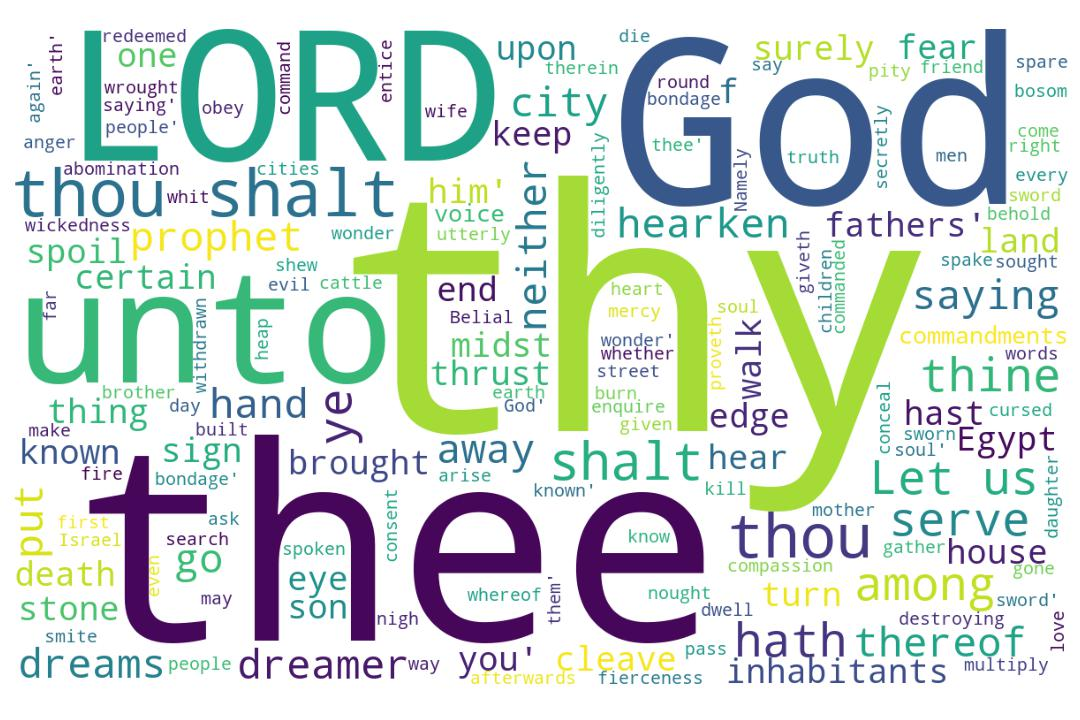
\includegraphics[width=\linewidth]{05OT-Deuteronomy/Deuteronomy13-WordCloud.jpg}
  \caption{Deuteronomy 13 Word Cloud}
  \label{fig:Deuteronomy 13 word Cloud}
\end{figure}

\marginpar{\scriptsize \centering \fcolorbox{bone}{lime}{\textbf{STAY TRUE}}\\ (Deuteronomy 13:1-22) \begin{compactenum}[I.][8]
    \item  A \textbf{Prophet with Signs }  \index[scripture]{Deuteronomy!Deu 13:01} \index[scripture]{Deuteronomy!Deu 13:03}\index[scripture]{Deuteronomy!Deu 13:05}(Deu 13:1, 3, 5)
    \item  The \textbf{Proof  of Sincerity}  \index[scripture]{Deuteronomy!Deu 13:03} (Deu 13:3)
    \item   \textbf{People gone Sideways}  \index[scripture]{Deuteronomy!Deu 13:07}\index[scripture]{Deuteronomy!Deu 13:09} (Deu 13:7, 9)
    \item   No \textbf{Pity or Sparing}  \index[scripture]{Deuteronomy!Deu 13:08}(Deu 13:8)
    \item   The \textbf{Pull to false Service}  \index[scripture]{Deuteronomy!Deu 13:13}(Deu 13:13)
    \item    \textbf{Punishment with Swords}  \index[scripture]{Deuteronomy!Deu 13:15}(Deu 13:15)
    \item    \textbf{Purging the Spoil}  \index[scripture]{Deuteronomy!Deu 13:16}(Deu 13:16)
\end{compactenum}}



\footnote{\textcolor[cmyk]{0.99998,1,0,0}{\hyperlink{TOC}{Return to end of Table of Contents.}}}\footnote{\href{https://audiobible.com/bible/deuteronomy_13.html}{\textcolor[cmyk]{0.99998,1,0,0}{Deuteronomy 13 Audio}}}\textcolor[cmyk]{0.99998,1,0,0}{If there arise among you \fcolorbox{bone}{lime}{a prophet}, or a dreamer of dreams, and giveth thee a sign or a wonder,}
[2] \textcolor[cmyk]{0.99998,1,0,0}{And the sign or the wonder come to pass, whereof he spake unto thee, saying, Let us go after other gods, which thou hast not known, and let us serve them;}
[3] \textcolor[cmyk]{0.99998,1,0,0}{Thou \fcolorbox{bone}{bone}{shalt} not hearken unto the words of that \fcolorbox{bone}{lime}{prophet}, or that dreamer of dreams: for the LORD your God \fcolorbox{bone}{lime}{proveth} you, to know whether ye love the LORD your God with all your heart and with all your soul.}
[4] \textcolor[cmyk]{0.99998,1,0,0}{Ye shall walk after the LORD your God, and fear him, and keep his commandments, and obey his voice, and ye shall serve him, and cleave unto him.}
[5] \textcolor[cmyk]{0.99998,1,0,0}{And that \fcolorbox{bone}{lime}{prophet}, or that dreamer of dreams, shall be put to death; because he hath spoken to turn \emph{you} away from the LORD your God, which brought you out of the land of Egypt, and redeemed you out of the house of bondage, to thrust thee out of the way which the LORD thy God commanded thee to walk in. So \fcolorbox{bone}{bone}{shalt} thou put the evil away from the midst of thee.}\\
\\
\P \textcolor[cmyk]{0.99998,1,0,0}{If thy brother, the son of thy mother, or thy son, or thy daughter, or the wife of thy bosom, or thy friend, which \emph{is} as thine own soul, entice thee secretly, saying, Let us go and serve other gods, which thou hast not known, thou, nor thy fathers;}
[7] \textcolor[cmyk]{0.99998,1,0,0}{\emph{Namely}, of the gods of the people which \emph{are} round about you, nigh unto thee, or far off from thee, from the \emph{one} end of the earth even unto the \emph{other} end of the earth;}
[8] \textcolor[cmyk]{0.99998,1,0,0}{Thou \fcolorbox{bone}{bone}{shalt} not consent unto him, nor hearken unto him; neither shall thine eye \fcolorbox{bone}{lime}{pity} him, neither \fcolorbox{bone}{bone}{shalt} thou spare, neither \fcolorbox{bone}{bone}{shalt} thou conceal him:}
[9] \textcolor[cmyk]{0.99998,1,0,0}{But thou \fcolorbox{bone}{bone}{shalt} surely kill him; thine hand shall be first upon him to put him to death, and afterwards the hand of all the people.}
[10] \textcolor[cmyk]{0.99998,1,0,0}{And thou \fcolorbox{bone}{bone}{shalt} stone him with stones, that he die; because he hath sought to thrust thee away from the LORD thy God, which brought thee out of the land of Egypt, from the house of bondage.}
[11] \textcolor[cmyk]{0.99998,1,0,0}{And all Israel shall hear, and fear, and shall do no more any such wickedness as this is among you.}\\
\\
\P \textcolor[cmyk]{0.99998,1,0,0}{If thou \fcolorbox{bone}{bone}{shalt} hear \emph{say} in one of thy cities, which the LORD thy God hath given thee to dwell there, saying,}
[13] \textcolor[cmyk]{0.99998,1,0,0}{\emph{Certain} men, the children of Belial, are gone out from among you, and have withdrawn the inhabitants of their city, saying, Let us go and serve other gods, which ye have not known;}
[14] \textcolor[cmyk]{0.99998,1,0,0}{Then \fcolorbox{bone}{bone}{shalt} thou enquire, and make search, and ask diligently; and, behold, \emph{if} \emph{it} \emph{be} truth, \emph{and} the thing certain, \emph{that} such abomination is wrought among you;}
[15] \textcolor[cmyk]{0.99998,1,0,0}{Thou \fcolorbox{bone}{bone}{shalt} surely smite the inhabitants of that city with the edge of the \fcolorbox{bone}{lime}{sword}, destroying it utterly, and all that \emph{is} therein, and the cattle thereof, with the edge of the sword.}
[16] \textcolor[cmyk]{0.99998,1,0,0}{And thou \fcolorbox{bone}{bone}{shalt} gather all the \fcolorbox{bone}{lime}{spoil} of it into the midst of the street thereof, and \fcolorbox{bone}{bone}{shalt} burn with fire the city, and all the \fcolorbox{bone}{lime}{spoil} thereof every whit, for the LORD thy God: and it shall be an heap for ever; it shall not be built again.}
[17] \textcolor[cmyk]{0.99998,1,0,0}{And there shall cleave nought of the cursed thing to thine hand: that the LORD may turn from the fierceness of his anger, and shew thee mercy, and have compassion upon thee, and multiply thee, as he hath sworn unto thy fathers;}
[18] \textcolor[cmyk]{0.99998,1,0,0}{When thou \fcolorbox{bone}{bone}{shalt} hearken to the voice of the LORD thy God, to keep all his commandments which I command thee this day, to do \emph{that} \emph{which} \emph{is} right in the eyes of the LORD thy God.}
\index[NWIV]{20!Deuteronomy!Deu 13:1}\index[AWIP]{If!Deuteronomy!Deu 13:1}\index[AWIP]{there!Deuteronomy!Deu 13:1}\index[AWIP]{arise!Deuteronomy!Deu 13:1}\index[AWIP]{among!Deuteronomy!Deu 13:1}\index[AWIP]{you!Deuteronomy!Deu 13:1}\index[AWIP]{a!Deuteronomy!Deu 13:1}\index[AWIP]{a!Deuteronomy!Deu 13:1 (2)}\index[AWIP]{a!Deuteronomy!Deu 13:1 (3)}\index[AWIP]{a!Deuteronomy!Deu 13:1 (4)}\index[AWIP]{prophet!Deuteronomy!Deu 13:1}\index[AWIP]{or!Deuteronomy!Deu 13:1}\index[AWIP]{or!Deuteronomy!Deu 13:1 (2)}\index[AWIP]{dreamer!Deuteronomy!Deu 13:1}\index[AWIP]{of!Deuteronomy!Deu 13:1}\index[AWIP]{dreams!Deuteronomy!Deu 13:1}\index[AWIP]{and!Deuteronomy!Deu 13:1}\index[AWIP]{giveth!Deuteronomy!Deu 13:1}\index[AWIP]{thee!Deuteronomy!Deu 13:1}\index[AWIP]{sign!Deuteronomy!Deu 13:1}\index[AWIP]{wonder!Deuteronomy!Deu 13:1}

\index[NWIV]{31!Deuteronomy!Deu 13:2}\index[AWIP]{And!Deuteronomy!Deu 13:2}\index[AWIP]{the!Deuteronomy!Deu 13:2}\index[AWIP]{the!Deuteronomy!Deu 13:2 (2)}\index[AWIP]{sign!Deuteronomy!Deu 13:2}\index[AWIP]{or!Deuteronomy!Deu 13:2}\index[AWIP]{wonder!Deuteronomy!Deu 13:2}\index[AWIP]{come!Deuteronomy!Deu 13:2}\index[AWIP]{to!Deuteronomy!Deu 13:2}\index[AWIP]{pass!Deuteronomy!Deu 13:2}\index[AWIP]{whereof!Deuteronomy!Deu 13:2}\index[AWIP]{he!Deuteronomy!Deu 13:2}\index[AWIP]{spake!Deuteronomy!Deu 13:2}\index[AWIP]{unto!Deuteronomy!Deu 13:2}\index[AWIP]{thee!Deuteronomy!Deu 13:2}\index[AWIP]{saying!Deuteronomy!Deu 13:2}\index[AWIP]{Let!Deuteronomy!Deu 13:2}\index[AWIP]{us!Deuteronomy!Deu 13:2}\index[AWIP]{us!Deuteronomy!Deu 13:2 (2)}\index[AWIP]{go!Deuteronomy!Deu 13:2}\index[AWIP]{after!Deuteronomy!Deu 13:2}\index[AWIP]{other!Deuteronomy!Deu 13:2}\index[AWIP]{gods!Deuteronomy!Deu 13:2}\index[AWIP]{which!Deuteronomy!Deu 13:2}\index[AWIP]{thou!Deuteronomy!Deu 13:2}\index[AWIP]{hast!Deuteronomy!Deu 13:2}\index[AWIP]{not!Deuteronomy!Deu 13:2}\index[AWIP]{known!Deuteronomy!Deu 13:2}\index[AWIP]{and!Deuteronomy!Deu 13:2}\index[AWIP]{let!Deuteronomy!Deu 13:2}\index[AWIP]{serve!Deuteronomy!Deu 13:2}\index[AWIP]{them!Deuteronomy!Deu 13:2}

\index[NWIV]{40!Deuteronomy!Deu 13:3}\index[AWIP]{Thou!Deuteronomy!Deu 13:3}\index[AWIP]{shalt!Deuteronomy!Deu 13:3}\index[AWIP]{not!Deuteronomy!Deu 13:3}\index[AWIP]{hearken!Deuteronomy!Deu 13:3}\index[AWIP]{unto!Deuteronomy!Deu 13:3}\index[AWIP]{the!Deuteronomy!Deu 13:3}\index[AWIP]{the!Deuteronomy!Deu 13:3 (2)}\index[AWIP]{the!Deuteronomy!Deu 13:3 (3)}\index[AWIP]{words!Deuteronomy!Deu 13:3}\index[AWIP]{of!Deuteronomy!Deu 13:3}\index[AWIP]{of!Deuteronomy!Deu 13:3 (2)}\index[AWIP]{that!Deuteronomy!Deu 13:3}\index[AWIP]{that!Deuteronomy!Deu 13:3 (2)}\index[AWIP]{prophet!Deuteronomy!Deu 13:3}\index[AWIP]{or!Deuteronomy!Deu 13:3}\index[AWIP]{dreamer!Deuteronomy!Deu 13:3}\index[AWIP]{dreams!Deuteronomy!Deu 13:3}\index[AWIP]{for!Deuteronomy!Deu 13:3}\index[AWIP]{LORD!Deuteronomy!Deu 13:3}\index[AWIP]{LORD!Deuteronomy!Deu 13:3 (2)}\index[AWIP]{your!Deuteronomy!Deu 13:3}\index[AWIP]{your!Deuteronomy!Deu 13:3 (2)}\index[AWIP]{your!Deuteronomy!Deu 13:3 (3)}\index[AWIP]{your!Deuteronomy!Deu 13:3 (4)}\index[AWIP]{God!Deuteronomy!Deu 13:3}\index[AWIP]{God!Deuteronomy!Deu 13:3 (2)}\index[AWIP]{proveth!Deuteronomy!Deu 13:3}\index[AWIP]{you!Deuteronomy!Deu 13:3}\index[AWIP]{to!Deuteronomy!Deu 13:3}\index[AWIP]{know!Deuteronomy!Deu 13:3}\index[AWIP]{whether!Deuteronomy!Deu 13:3}\index[AWIP]{ye!Deuteronomy!Deu 13:3}\index[AWIP]{love!Deuteronomy!Deu 13:3}\index[AWIP]{with!Deuteronomy!Deu 13:3}\index[AWIP]{with!Deuteronomy!Deu 13:3 (2)}\index[AWIP]{all!Deuteronomy!Deu 13:3}\index[AWIP]{all!Deuteronomy!Deu 13:3 (2)}\index[AWIP]{heart!Deuteronomy!Deu 13:3}\index[AWIP]{and!Deuteronomy!Deu 13:3}\index[AWIP]{soul!Deuteronomy!Deu 13:3}

\index[NWIV]{28!Deuteronomy!Deu 13:4}\index[AWIP]{Ye!Deuteronomy!Deu 13:4}\index[AWIP]{shall!Deuteronomy!Deu 13:4}\index[AWIP]{shall!Deuteronomy!Deu 13:4 (2)}\index[AWIP]{walk!Deuteronomy!Deu 13:4}\index[AWIP]{after!Deuteronomy!Deu 13:4}\index[AWIP]{the!Deuteronomy!Deu 13:4}\index[AWIP]{LORD!Deuteronomy!Deu 13:4}\index[AWIP]{your!Deuteronomy!Deu 13:4}\index[AWIP]{God!Deuteronomy!Deu 13:4}\index[AWIP]{and!Deuteronomy!Deu 13:4}\index[AWIP]{and!Deuteronomy!Deu 13:4 (2)}\index[AWIP]{and!Deuteronomy!Deu 13:4 (3)}\index[AWIP]{and!Deuteronomy!Deu 13:4 (4)}\index[AWIP]{and!Deuteronomy!Deu 13:4 (5)}\index[AWIP]{fear!Deuteronomy!Deu 13:4}\index[AWIP]{him!Deuteronomy!Deu 13:4}\index[AWIP]{him!Deuteronomy!Deu 13:4 (2)}\index[AWIP]{him!Deuteronomy!Deu 13:4 (3)}\index[AWIP]{keep!Deuteronomy!Deu 13:4}\index[AWIP]{his!Deuteronomy!Deu 13:4}\index[AWIP]{his!Deuteronomy!Deu 13:4 (2)}\index[AWIP]{commandments!Deuteronomy!Deu 13:4}\index[AWIP]{obey!Deuteronomy!Deu 13:4}\index[AWIP]{voice!Deuteronomy!Deu 13:4}\index[AWIP]{ye!Deuteronomy!Deu 13:4}\index[AWIP]{serve!Deuteronomy!Deu 13:4}\index[AWIP]{cleave!Deuteronomy!Deu 13:4}\index[AWIP]{unto!Deuteronomy!Deu 13:4}

\index[NWIV]{73!Deuteronomy!Deu 13:5}\index[AWIP]{And!Deuteronomy!Deu 13:5}\index[AWIP]{that!Deuteronomy!Deu 13:5}\index[AWIP]{that!Deuteronomy!Deu 13:5 (2)}\index[AWIP]{prophet!Deuteronomy!Deu 13:5}\index[AWIP]{or!Deuteronomy!Deu 13:5}\index[AWIP]{dreamer!Deuteronomy!Deu 13:5}\index[AWIP]{of!Deuteronomy!Deu 13:5}\index[AWIP]{of!Deuteronomy!Deu 13:5 (2)}\index[AWIP]{of!Deuteronomy!Deu 13:5 (3)}\index[AWIP]{of!Deuteronomy!Deu 13:5 (4)}\index[AWIP]{of!Deuteronomy!Deu 13:5 (5)}\index[AWIP]{of!Deuteronomy!Deu 13:5 (6)}\index[AWIP]{of!Deuteronomy!Deu 13:5 (7)}\index[AWIP]{dreams!Deuteronomy!Deu 13:5}\index[AWIP]{shall!Deuteronomy!Deu 13:5}\index[AWIP]{be!Deuteronomy!Deu 13:5}\index[AWIP]{put!Deuteronomy!Deu 13:5}\index[AWIP]{put!Deuteronomy!Deu 13:5 (2)}\index[AWIP]{to!Deuteronomy!Deu 13:5}\index[AWIP]{to!Deuteronomy!Deu 13:5 (2)}\index[AWIP]{to!Deuteronomy!Deu 13:5 (3)}\index[AWIP]{to!Deuteronomy!Deu 13:5 (4)}\index[AWIP]{death!Deuteronomy!Deu 13:5}\index[AWIP]{because!Deuteronomy!Deu 13:5}\index[AWIP]{he!Deuteronomy!Deu 13:5}\index[AWIP]{hath!Deuteronomy!Deu 13:5}\index[AWIP]{spoken!Deuteronomy!Deu 13:5}\index[AWIP]{turn!Deuteronomy!Deu 13:5}\index[AWIP]{\emph{you}!Deuteronomy!Deu 13:5}\index[AWIP]{away!Deuteronomy!Deu 13:5}\index[AWIP]{away!Deuteronomy!Deu 13:5 (2)}\index[AWIP]{from!Deuteronomy!Deu 13:5}\index[AWIP]{from!Deuteronomy!Deu 13:5 (2)}\index[AWIP]{the!Deuteronomy!Deu 13:5}\index[AWIP]{the!Deuteronomy!Deu 13:5 (2)}\index[AWIP]{the!Deuteronomy!Deu 13:5 (3)}\index[AWIP]{the!Deuteronomy!Deu 13:5 (4)}\index[AWIP]{the!Deuteronomy!Deu 13:5 (5)}\index[AWIP]{the!Deuteronomy!Deu 13:5 (6)}\index[AWIP]{the!Deuteronomy!Deu 13:5 (7)}\index[AWIP]{LORD!Deuteronomy!Deu 13:5}\index[AWIP]{LORD!Deuteronomy!Deu 13:5 (2)}\index[AWIP]{your!Deuteronomy!Deu 13:5}\index[AWIP]{God!Deuteronomy!Deu 13:5}\index[AWIP]{God!Deuteronomy!Deu 13:5 (2)}\index[AWIP]{which!Deuteronomy!Deu 13:5}\index[AWIP]{which!Deuteronomy!Deu 13:5 (2)}\index[AWIP]{brought!Deuteronomy!Deu 13:5}\index[AWIP]{you!Deuteronomy!Deu 13:5}\index[AWIP]{you!Deuteronomy!Deu 13:5 (2)}\index[AWIP]{out!Deuteronomy!Deu 13:5}\index[AWIP]{out!Deuteronomy!Deu 13:5 (2)}\index[AWIP]{out!Deuteronomy!Deu 13:5 (3)}\index[AWIP]{land!Deuteronomy!Deu 13:5}\index[AWIP]{Egypt!Deuteronomy!Deu 13:5}\index[AWIP]{and!Deuteronomy!Deu 13:5}\index[AWIP]{redeemed!Deuteronomy!Deu 13:5}\index[AWIP]{house!Deuteronomy!Deu 13:5}\index[AWIP]{bondage!Deuteronomy!Deu 13:5}\index[AWIP]{thrust!Deuteronomy!Deu 13:5}\index[AWIP]{thee!Deuteronomy!Deu 13:5}\index[AWIP]{thee!Deuteronomy!Deu 13:5 (2)}\index[AWIP]{thee!Deuteronomy!Deu 13:5 (3)}\index[AWIP]{way!Deuteronomy!Deu 13:5}\index[AWIP]{thy!Deuteronomy!Deu 13:5}\index[AWIP]{commanded!Deuteronomy!Deu 13:5}\index[AWIP]{walk!Deuteronomy!Deu 13:5}\index[AWIP]{in!Deuteronomy!Deu 13:5}\index[AWIP]{So!Deuteronomy!Deu 13:5}\index[AWIP]{shalt!Deuteronomy!Deu 13:5}\index[AWIP]{thou!Deuteronomy!Deu 13:5}\index[AWIP]{evil!Deuteronomy!Deu 13:5}\index[AWIP]{midst!Deuteronomy!Deu 13:5}\index[AWIP]{\emph{you}!Deuteronomy!Deu 13:5}

\index[NWIV]{49!Deuteronomy!Deu 13:6}\index[AWIP]{f!Deuteronomy!Deu 13:6}\index[AWIP]{thy!Deuteronomy!Deu 13:6}\index[AWIP]{thy!Deuteronomy!Deu 13:6 (2)}\index[AWIP]{thy!Deuteronomy!Deu 13:6 (3)}\index[AWIP]{thy!Deuteronomy!Deu 13:6 (4)}\index[AWIP]{thy!Deuteronomy!Deu 13:6 (5)}\index[AWIP]{thy!Deuteronomy!Deu 13:6 (6)}\index[AWIP]{thy!Deuteronomy!Deu 13:6 (7)}\index[AWIP]{brother!Deuteronomy!Deu 13:6}\index[AWIP]{the!Deuteronomy!Deu 13:6}\index[AWIP]{the!Deuteronomy!Deu 13:6 (2)}\index[AWIP]{son!Deuteronomy!Deu 13:6}\index[AWIP]{son!Deuteronomy!Deu 13:6 (2)}\index[AWIP]{of!Deuteronomy!Deu 13:6}\index[AWIP]{of!Deuteronomy!Deu 13:6 (2)}\index[AWIP]{mother!Deuteronomy!Deu 13:6}\index[AWIP]{or!Deuteronomy!Deu 13:6}\index[AWIP]{or!Deuteronomy!Deu 13:6 (2)}\index[AWIP]{or!Deuteronomy!Deu 13:6 (3)}\index[AWIP]{or!Deuteronomy!Deu 13:6 (4)}\index[AWIP]{daughter!Deuteronomy!Deu 13:6}\index[AWIP]{wife!Deuteronomy!Deu 13:6}\index[AWIP]{bosom!Deuteronomy!Deu 13:6}\index[AWIP]{friend!Deuteronomy!Deu 13:6}\index[AWIP]{which!Deuteronomy!Deu 13:6}\index[AWIP]{which!Deuteronomy!Deu 13:6 (2)}\index[AWIP]{\emph{is}!Deuteronomy!Deu 13:6}\index[AWIP]{as!Deuteronomy!Deu 13:6}\index[AWIP]{thine!Deuteronomy!Deu 13:6}\index[AWIP]{own!Deuteronomy!Deu 13:6}\index[AWIP]{soul!Deuteronomy!Deu 13:6}\index[AWIP]{entice!Deuteronomy!Deu 13:6}\index[AWIP]{thee!Deuteronomy!Deu 13:6}\index[AWIP]{secretly!Deuteronomy!Deu 13:6}\index[AWIP]{saying!Deuteronomy!Deu 13:6}\index[AWIP]{Let!Deuteronomy!Deu 13:6}\index[AWIP]{us!Deuteronomy!Deu 13:6}\index[AWIP]{go!Deuteronomy!Deu 13:6}\index[AWIP]{and!Deuteronomy!Deu 13:6}\index[AWIP]{serve!Deuteronomy!Deu 13:6}\index[AWIP]{other!Deuteronomy!Deu 13:6}\index[AWIP]{gods!Deuteronomy!Deu 13:6}\index[AWIP]{thou!Deuteronomy!Deu 13:6}\index[AWIP]{thou!Deuteronomy!Deu 13:6 (2)}\index[AWIP]{hast!Deuteronomy!Deu 13:6}\index[AWIP]{not!Deuteronomy!Deu 13:6}\index[AWIP]{known!Deuteronomy!Deu 13:6}\index[AWIP]{nor!Deuteronomy!Deu 13:6}\index[AWIP]{fathers!Deuteronomy!Deu 13:6}\index[AWIP]{\emph{is}!Deuteronomy!Deu 13:6}

\index[NWIV]{35!Deuteronomy!Deu 13:7}\index[AWIP]{\emph{Namely}!Deuteronomy!Deu 13:7}\index[AWIP]{of!Deuteronomy!Deu 13:7}\index[AWIP]{of!Deuteronomy!Deu 13:7 (2)}\index[AWIP]{of!Deuteronomy!Deu 13:7 (3)}\index[AWIP]{of!Deuteronomy!Deu 13:7 (4)}\index[AWIP]{the!Deuteronomy!Deu 13:7}\index[AWIP]{the!Deuteronomy!Deu 13:7 (2)}\index[AWIP]{the!Deuteronomy!Deu 13:7 (3)}\index[AWIP]{the!Deuteronomy!Deu 13:7 (4)}\index[AWIP]{the!Deuteronomy!Deu 13:7 (5)}\index[AWIP]{the!Deuteronomy!Deu 13:7 (6)}\index[AWIP]{gods!Deuteronomy!Deu 13:7}\index[AWIP]{people!Deuteronomy!Deu 13:7}\index[AWIP]{which!Deuteronomy!Deu 13:7}\index[AWIP]{\emph{are}!Deuteronomy!Deu 13:7}\index[AWIP]{round!Deuteronomy!Deu 13:7}\index[AWIP]{about!Deuteronomy!Deu 13:7}\index[AWIP]{you!Deuteronomy!Deu 13:7}\index[AWIP]{nigh!Deuteronomy!Deu 13:7}\index[AWIP]{unto!Deuteronomy!Deu 13:7}\index[AWIP]{unto!Deuteronomy!Deu 13:7 (2)}\index[AWIP]{thee!Deuteronomy!Deu 13:7}\index[AWIP]{thee!Deuteronomy!Deu 13:7 (2)}\index[AWIP]{or!Deuteronomy!Deu 13:7}\index[AWIP]{far!Deuteronomy!Deu 13:7}\index[AWIP]{off!Deuteronomy!Deu 13:7}\index[AWIP]{from!Deuteronomy!Deu 13:7}\index[AWIP]{from!Deuteronomy!Deu 13:7 (2)}\index[AWIP]{\emph{one}!Deuteronomy!Deu 13:7}\index[AWIP]{end!Deuteronomy!Deu 13:7}\index[AWIP]{end!Deuteronomy!Deu 13:7 (2)}\index[AWIP]{earth!Deuteronomy!Deu 13:7}\index[AWIP]{earth!Deuteronomy!Deu 13:7 (2)}\index[AWIP]{even!Deuteronomy!Deu 13:7}\index[AWIP]{\emph{other}!Deuteronomy!Deu 13:7}\index[AWIP]{\emph{Namely}!Deuteronomy!Deu 13:7}\index[AWIP]{\emph{are}!Deuteronomy!Deu 13:7}\index[AWIP]{\emph{one}!Deuteronomy!Deu 13:7}\index[AWIP]{\emph{other}!Deuteronomy!Deu 13:7}

\index[NWIV]{25!Deuteronomy!Deu 13:8}\index[AWIP]{Thou!Deuteronomy!Deu 13:8}\index[AWIP]{shalt!Deuteronomy!Deu 13:8}\index[AWIP]{shalt!Deuteronomy!Deu 13:8 (2)}\index[AWIP]{shalt!Deuteronomy!Deu 13:8 (3)}\index[AWIP]{not!Deuteronomy!Deu 13:8}\index[AWIP]{consent!Deuteronomy!Deu 13:8}\index[AWIP]{unto!Deuteronomy!Deu 13:8}\index[AWIP]{unto!Deuteronomy!Deu 13:8 (2)}\index[AWIP]{him!Deuteronomy!Deu 13:8}\index[AWIP]{him!Deuteronomy!Deu 13:8 (2)}\index[AWIP]{him!Deuteronomy!Deu 13:8 (3)}\index[AWIP]{him!Deuteronomy!Deu 13:8 (4)}\index[AWIP]{nor!Deuteronomy!Deu 13:8}\index[AWIP]{hearken!Deuteronomy!Deu 13:8}\index[AWIP]{neither!Deuteronomy!Deu 13:8}\index[AWIP]{neither!Deuteronomy!Deu 13:8 (2)}\index[AWIP]{neither!Deuteronomy!Deu 13:8 (3)}\index[AWIP]{shall!Deuteronomy!Deu 13:8}\index[AWIP]{thine!Deuteronomy!Deu 13:8}\index[AWIP]{eye!Deuteronomy!Deu 13:8}\index[AWIP]{pity!Deuteronomy!Deu 13:8}\index[AWIP]{thou!Deuteronomy!Deu 13:8}\index[AWIP]{thou!Deuteronomy!Deu 13:8 (2)}\index[AWIP]{spare!Deuteronomy!Deu 13:8}\index[AWIP]{conceal!Deuteronomy!Deu 13:8}

\index[NWIV]{26!Deuteronomy!Deu 13:9}\index[AWIP]{But!Deuteronomy!Deu 13:9}\index[AWIP]{thou!Deuteronomy!Deu 13:9}\index[AWIP]{shalt!Deuteronomy!Deu 13:9}\index[AWIP]{surely!Deuteronomy!Deu 13:9}\index[AWIP]{kill!Deuteronomy!Deu 13:9}\index[AWIP]{him!Deuteronomy!Deu 13:9}\index[AWIP]{him!Deuteronomy!Deu 13:9 (2)}\index[AWIP]{him!Deuteronomy!Deu 13:9 (3)}\index[AWIP]{thine!Deuteronomy!Deu 13:9}\index[AWIP]{hand!Deuteronomy!Deu 13:9}\index[AWIP]{hand!Deuteronomy!Deu 13:9 (2)}\index[AWIP]{shall!Deuteronomy!Deu 13:9}\index[AWIP]{be!Deuteronomy!Deu 13:9}\index[AWIP]{first!Deuteronomy!Deu 13:9}\index[AWIP]{upon!Deuteronomy!Deu 13:9}\index[AWIP]{to!Deuteronomy!Deu 13:9}\index[AWIP]{to!Deuteronomy!Deu 13:9 (2)}\index[AWIP]{put!Deuteronomy!Deu 13:9}\index[AWIP]{death!Deuteronomy!Deu 13:9}\index[AWIP]{and!Deuteronomy!Deu 13:9}\index[AWIP]{afterwards!Deuteronomy!Deu 13:9}\index[AWIP]{the!Deuteronomy!Deu 13:9}\index[AWIP]{the!Deuteronomy!Deu 13:9 (2)}\index[AWIP]{of!Deuteronomy!Deu 13:9}\index[AWIP]{all!Deuteronomy!Deu 13:9}\index[AWIP]{people!Deuteronomy!Deu 13:9}

\index[NWIV]{37!Deuteronomy!Deu 13:10}\index[AWIP]{And!Deuteronomy!Deu 13:10}\index[AWIP]{thou!Deuteronomy!Deu 13:10}\index[AWIP]{shalt!Deuteronomy!Deu 13:10}\index[AWIP]{stone!Deuteronomy!Deu 13:10}\index[AWIP]{him!Deuteronomy!Deu 13:10}\index[AWIP]{with!Deuteronomy!Deu 13:10}\index[AWIP]{stones!Deuteronomy!Deu 13:10}\index[AWIP]{that!Deuteronomy!Deu 13:10}\index[AWIP]{he!Deuteronomy!Deu 13:10}\index[AWIP]{he!Deuteronomy!Deu 13:10 (2)}\index[AWIP]{die!Deuteronomy!Deu 13:10}\index[AWIP]{because!Deuteronomy!Deu 13:10}\index[AWIP]{hath!Deuteronomy!Deu 13:10}\index[AWIP]{sought!Deuteronomy!Deu 13:10}\index[AWIP]{to!Deuteronomy!Deu 13:10}\index[AWIP]{thrust!Deuteronomy!Deu 13:10}\index[AWIP]{thee!Deuteronomy!Deu 13:10}\index[AWIP]{thee!Deuteronomy!Deu 13:10 (2)}\index[AWIP]{away!Deuteronomy!Deu 13:10}\index[AWIP]{from!Deuteronomy!Deu 13:10}\index[AWIP]{from!Deuteronomy!Deu 13:10 (2)}\index[AWIP]{the!Deuteronomy!Deu 13:10}\index[AWIP]{the!Deuteronomy!Deu 13:10 (2)}\index[AWIP]{the!Deuteronomy!Deu 13:10 (3)}\index[AWIP]{LORD!Deuteronomy!Deu 13:10}\index[AWIP]{thy!Deuteronomy!Deu 13:10}\index[AWIP]{God!Deuteronomy!Deu 13:10}\index[AWIP]{which!Deuteronomy!Deu 13:10}\index[AWIP]{brought!Deuteronomy!Deu 13:10}\index[AWIP]{out!Deuteronomy!Deu 13:10}\index[AWIP]{of!Deuteronomy!Deu 13:10}\index[AWIP]{of!Deuteronomy!Deu 13:10 (2)}\index[AWIP]{of!Deuteronomy!Deu 13:10 (3)}\index[AWIP]{land!Deuteronomy!Deu 13:10}\index[AWIP]{Egypt!Deuteronomy!Deu 13:10}\index[AWIP]{house!Deuteronomy!Deu 13:10}\index[AWIP]{bondage!Deuteronomy!Deu 13:10}

\index[NWIV]{20!Deuteronomy!Deu 13:11}\index[AWIP]{And!Deuteronomy!Deu 13:11}\index[AWIP]{all!Deuteronomy!Deu 13:11}\index[AWIP]{Israel!Deuteronomy!Deu 13:11}\index[AWIP]{shall!Deuteronomy!Deu 13:11}\index[AWIP]{shall!Deuteronomy!Deu 13:11 (2)}\index[AWIP]{hear!Deuteronomy!Deu 13:11}\index[AWIP]{and!Deuteronomy!Deu 13:11}\index[AWIP]{and!Deuteronomy!Deu 13:11 (2)}\index[AWIP]{fear!Deuteronomy!Deu 13:11}\index[AWIP]{do!Deuteronomy!Deu 13:11}\index[AWIP]{no!Deuteronomy!Deu 13:11}\index[AWIP]{more!Deuteronomy!Deu 13:11}\index[AWIP]{any!Deuteronomy!Deu 13:11}\index[AWIP]{such!Deuteronomy!Deu 13:11}\index[AWIP]{wickedness!Deuteronomy!Deu 13:11}\index[AWIP]{as!Deuteronomy!Deu 13:11}\index[AWIP]{this!Deuteronomy!Deu 13:11}\index[AWIP]{is!Deuteronomy!Deu 13:11}\index[AWIP]{among!Deuteronomy!Deu 13:11}\index[AWIP]{you!Deuteronomy!Deu 13:11}

\index[NWIV]{22!Deuteronomy!Deu 13:12}\index[AWIP]{f!Deuteronomy!Deu 13:12}\index[AWIP]{thou!Deuteronomy!Deu 13:12}\index[AWIP]{shalt!Deuteronomy!Deu 13:12}\index[AWIP]{hear!Deuteronomy!Deu 13:12}\index[AWIP]{\emph{say}!Deuteronomy!Deu 13:12}\index[AWIP]{in!Deuteronomy!Deu 13:12}\index[AWIP]{one!Deuteronomy!Deu 13:12}\index[AWIP]{of!Deuteronomy!Deu 13:12}\index[AWIP]{thy!Deuteronomy!Deu 13:12}\index[AWIP]{thy!Deuteronomy!Deu 13:12 (2)}\index[AWIP]{cities!Deuteronomy!Deu 13:12}\index[AWIP]{which!Deuteronomy!Deu 13:12}\index[AWIP]{the!Deuteronomy!Deu 13:12}\index[AWIP]{LORD!Deuteronomy!Deu 13:12}\index[AWIP]{God!Deuteronomy!Deu 13:12}\index[AWIP]{hath!Deuteronomy!Deu 13:12}\index[AWIP]{given!Deuteronomy!Deu 13:12}\index[AWIP]{thee!Deuteronomy!Deu 13:12}\index[AWIP]{to!Deuteronomy!Deu 13:12}\index[AWIP]{dwell!Deuteronomy!Deu 13:12}\index[AWIP]{there!Deuteronomy!Deu 13:12}\index[AWIP]{saying!Deuteronomy!Deu 13:12}\index[AWIP]{\emph{say}!Deuteronomy!Deu 13:12}

\index[NWIV]{33!Deuteronomy!Deu 13:13}\index[AWIP]{\emph{Certain}!Deuteronomy!Deu 13:13}\index[AWIP]{men!Deuteronomy!Deu 13:13}\index[AWIP]{the!Deuteronomy!Deu 13:13}\index[AWIP]{the!Deuteronomy!Deu 13:13 (2)}\index[AWIP]{children!Deuteronomy!Deu 13:13}\index[AWIP]{of!Deuteronomy!Deu 13:13}\index[AWIP]{of!Deuteronomy!Deu 13:13 (2)}\index[AWIP]{Belial!Deuteronomy!Deu 13:13}\index[AWIP]{are!Deuteronomy!Deu 13:13}\index[AWIP]{gone!Deuteronomy!Deu 13:13}\index[AWIP]{out!Deuteronomy!Deu 13:13}\index[AWIP]{from!Deuteronomy!Deu 13:13}\index[AWIP]{among!Deuteronomy!Deu 13:13}\index[AWIP]{you!Deuteronomy!Deu 13:13}\index[AWIP]{and!Deuteronomy!Deu 13:13}\index[AWIP]{and!Deuteronomy!Deu 13:13 (2)}\index[AWIP]{have!Deuteronomy!Deu 13:13}\index[AWIP]{have!Deuteronomy!Deu 13:13 (2)}\index[AWIP]{withdrawn!Deuteronomy!Deu 13:13}\index[AWIP]{inhabitants!Deuteronomy!Deu 13:13}\index[AWIP]{their!Deuteronomy!Deu 13:13}\index[AWIP]{city!Deuteronomy!Deu 13:13}\index[AWIP]{saying!Deuteronomy!Deu 13:13}\index[AWIP]{Let!Deuteronomy!Deu 13:13}\index[AWIP]{us!Deuteronomy!Deu 13:13}\index[AWIP]{go!Deuteronomy!Deu 13:13}\index[AWIP]{serve!Deuteronomy!Deu 13:13}\index[AWIP]{other!Deuteronomy!Deu 13:13}\index[AWIP]{gods!Deuteronomy!Deu 13:13}\index[AWIP]{which!Deuteronomy!Deu 13:13}\index[AWIP]{ye!Deuteronomy!Deu 13:13}\index[AWIP]{not!Deuteronomy!Deu 13:13}\index[AWIP]{known!Deuteronomy!Deu 13:13}\index[AWIP]{\emph{Certain}!Deuteronomy!Deu 13:13}

\index[NWIV]{27!Deuteronomy!Deu 13:14}\index[AWIP]{Then!Deuteronomy!Deu 13:14}\index[AWIP]{shalt!Deuteronomy!Deu 13:14}\index[AWIP]{thou!Deuteronomy!Deu 13:14}\index[AWIP]{enquire!Deuteronomy!Deu 13:14}\index[AWIP]{and!Deuteronomy!Deu 13:14}\index[AWIP]{and!Deuteronomy!Deu 13:14 (2)}\index[AWIP]{and!Deuteronomy!Deu 13:14 (3)}\index[AWIP]{make!Deuteronomy!Deu 13:14}\index[AWIP]{search!Deuteronomy!Deu 13:14}\index[AWIP]{ask!Deuteronomy!Deu 13:14}\index[AWIP]{diligently!Deuteronomy!Deu 13:14}\index[AWIP]{behold!Deuteronomy!Deu 13:14}\index[AWIP]{\emph{if}!Deuteronomy!Deu 13:14}\index[AWIP]{\emph{it}!Deuteronomy!Deu 13:14}\index[AWIP]{\emph{be}!Deuteronomy!Deu 13:14}\index[AWIP]{truth!Deuteronomy!Deu 13:14}\index[AWIP]{\emph{and}!Deuteronomy!Deu 13:14}\index[AWIP]{the!Deuteronomy!Deu 13:14}\index[AWIP]{thing!Deuteronomy!Deu 13:14}\index[AWIP]{certain!Deuteronomy!Deu 13:14}\index[AWIP]{\emph{that}!Deuteronomy!Deu 13:14}\index[AWIP]{such!Deuteronomy!Deu 13:14}\index[AWIP]{abomination!Deuteronomy!Deu 13:14}\index[AWIP]{is!Deuteronomy!Deu 13:14}\index[AWIP]{wrought!Deuteronomy!Deu 13:14}\index[AWIP]{among!Deuteronomy!Deu 13:14}\index[AWIP]{you!Deuteronomy!Deu 13:14}\index[AWIP]{\emph{if}!Deuteronomy!Deu 13:14}\index[AWIP]{\emph{it}!Deuteronomy!Deu 13:14}\index[AWIP]{\emph{be}!Deuteronomy!Deu 13:14}\index[AWIP]{\emph{and}!Deuteronomy!Deu 13:14}\index[AWIP]{\emph{that}!Deuteronomy!Deu 13:14}

\index[NWIV]{33!Deuteronomy!Deu 13:15}\index[AWIP]{Thou!Deuteronomy!Deu 13:15}\index[AWIP]{shalt!Deuteronomy!Deu 13:15}\index[AWIP]{surely!Deuteronomy!Deu 13:15}\index[AWIP]{smite!Deuteronomy!Deu 13:15}\index[AWIP]{the!Deuteronomy!Deu 13:15}\index[AWIP]{the!Deuteronomy!Deu 13:15 (2)}\index[AWIP]{the!Deuteronomy!Deu 13:15 (3)}\index[AWIP]{the!Deuteronomy!Deu 13:15 (4)}\index[AWIP]{the!Deuteronomy!Deu 13:15 (5)}\index[AWIP]{the!Deuteronomy!Deu 13:15 (6)}\index[AWIP]{inhabitants!Deuteronomy!Deu 13:15}\index[AWIP]{of!Deuteronomy!Deu 13:15}\index[AWIP]{of!Deuteronomy!Deu 13:15 (2)}\index[AWIP]{of!Deuteronomy!Deu 13:15 (3)}\index[AWIP]{that!Deuteronomy!Deu 13:15}\index[AWIP]{that!Deuteronomy!Deu 13:15 (2)}\index[AWIP]{city!Deuteronomy!Deu 13:15}\index[AWIP]{with!Deuteronomy!Deu 13:15}\index[AWIP]{with!Deuteronomy!Deu 13:15 (2)}\index[AWIP]{edge!Deuteronomy!Deu 13:15}\index[AWIP]{edge!Deuteronomy!Deu 13:15 (2)}\index[AWIP]{sword!Deuteronomy!Deu 13:15}\index[AWIP]{sword!Deuteronomy!Deu 13:15 (2)}\index[AWIP]{destroying!Deuteronomy!Deu 13:15}\index[AWIP]{it!Deuteronomy!Deu 13:15}\index[AWIP]{utterly!Deuteronomy!Deu 13:15}\index[AWIP]{and!Deuteronomy!Deu 13:15}\index[AWIP]{and!Deuteronomy!Deu 13:15 (2)}\index[AWIP]{all!Deuteronomy!Deu 13:15}\index[AWIP]{\emph{is}!Deuteronomy!Deu 13:15}\index[AWIP]{therein!Deuteronomy!Deu 13:15}\index[AWIP]{cattle!Deuteronomy!Deu 13:15}\index[AWIP]{thereof!Deuteronomy!Deu 13:15}\index[AWIP]{\emph{is}!Deuteronomy!Deu 13:15}

\index[NWIV]{49!Deuteronomy!Deu 13:16}\index[AWIP]{And!Deuteronomy!Deu 13:16}\index[AWIP]{thou!Deuteronomy!Deu 13:16}\index[AWIP]{shalt!Deuteronomy!Deu 13:16}\index[AWIP]{shalt!Deuteronomy!Deu 13:16 (2)}\index[AWIP]{gather!Deuteronomy!Deu 13:16}\index[AWIP]{all!Deuteronomy!Deu 13:16}\index[AWIP]{all!Deuteronomy!Deu 13:16 (2)}\index[AWIP]{the!Deuteronomy!Deu 13:16}\index[AWIP]{the!Deuteronomy!Deu 13:16 (2)}\index[AWIP]{the!Deuteronomy!Deu 13:16 (3)}\index[AWIP]{the!Deuteronomy!Deu 13:16 (4)}\index[AWIP]{the!Deuteronomy!Deu 13:16 (5)}\index[AWIP]{the!Deuteronomy!Deu 13:16 (6)}\index[AWIP]{spoil!Deuteronomy!Deu 13:16}\index[AWIP]{spoil!Deuteronomy!Deu 13:16 (2)}\index[AWIP]{of!Deuteronomy!Deu 13:16}\index[AWIP]{of!Deuteronomy!Deu 13:16 (2)}\index[AWIP]{it!Deuteronomy!Deu 13:16}\index[AWIP]{it!Deuteronomy!Deu 13:16 (2)}\index[AWIP]{it!Deuteronomy!Deu 13:16 (3)}\index[AWIP]{into!Deuteronomy!Deu 13:16}\index[AWIP]{midst!Deuteronomy!Deu 13:16}\index[AWIP]{street!Deuteronomy!Deu 13:16}\index[AWIP]{thereof!Deuteronomy!Deu 13:16}\index[AWIP]{thereof!Deuteronomy!Deu 13:16 (2)}\index[AWIP]{and!Deuteronomy!Deu 13:16}\index[AWIP]{and!Deuteronomy!Deu 13:16 (2)}\index[AWIP]{and!Deuteronomy!Deu 13:16 (3)}\index[AWIP]{burn!Deuteronomy!Deu 13:16}\index[AWIP]{with!Deuteronomy!Deu 13:16}\index[AWIP]{fire!Deuteronomy!Deu 13:16}\index[AWIP]{city!Deuteronomy!Deu 13:16}\index[AWIP]{every!Deuteronomy!Deu 13:16}\index[AWIP]{whit!Deuteronomy!Deu 13:16}\index[AWIP]{for!Deuteronomy!Deu 13:16}\index[AWIP]{for!Deuteronomy!Deu 13:16 (2)}\index[AWIP]{LORD!Deuteronomy!Deu 13:16}\index[AWIP]{thy!Deuteronomy!Deu 13:16}\index[AWIP]{God!Deuteronomy!Deu 13:16}\index[AWIP]{shall!Deuteronomy!Deu 13:16}\index[AWIP]{shall!Deuteronomy!Deu 13:16 (2)}\index[AWIP]{be!Deuteronomy!Deu 13:16}\index[AWIP]{be!Deuteronomy!Deu 13:16 (2)}\index[AWIP]{an!Deuteronomy!Deu 13:16}\index[AWIP]{heap!Deuteronomy!Deu 13:16}\index[AWIP]{ever!Deuteronomy!Deu 13:16}\index[AWIP]{not!Deuteronomy!Deu 13:16}\index[AWIP]{built!Deuteronomy!Deu 13:16}\index[AWIP]{again!Deuteronomy!Deu 13:16}

\index[NWIV]{42!Deuteronomy!Deu 13:17}\index[AWIP]{And!Deuteronomy!Deu 13:17}\index[AWIP]{there!Deuteronomy!Deu 13:17}\index[AWIP]{shall!Deuteronomy!Deu 13:17}\index[AWIP]{cleave!Deuteronomy!Deu 13:17}\index[AWIP]{nought!Deuteronomy!Deu 13:17}\index[AWIP]{of!Deuteronomy!Deu 13:17}\index[AWIP]{of!Deuteronomy!Deu 13:17 (2)}\index[AWIP]{the!Deuteronomy!Deu 13:17}\index[AWIP]{the!Deuteronomy!Deu 13:17 (2)}\index[AWIP]{the!Deuteronomy!Deu 13:17 (3)}\index[AWIP]{cursed!Deuteronomy!Deu 13:17}\index[AWIP]{thing!Deuteronomy!Deu 13:17}\index[AWIP]{to!Deuteronomy!Deu 13:17}\index[AWIP]{thine!Deuteronomy!Deu 13:17}\index[AWIP]{hand!Deuteronomy!Deu 13:17}\index[AWIP]{that!Deuteronomy!Deu 13:17}\index[AWIP]{LORD!Deuteronomy!Deu 13:17}\index[AWIP]{may!Deuteronomy!Deu 13:17}\index[AWIP]{turn!Deuteronomy!Deu 13:17}\index[AWIP]{from!Deuteronomy!Deu 13:17}\index[AWIP]{fierceness!Deuteronomy!Deu 13:17}\index[AWIP]{his!Deuteronomy!Deu 13:17}\index[AWIP]{anger!Deuteronomy!Deu 13:17}\index[AWIP]{and!Deuteronomy!Deu 13:17}\index[AWIP]{and!Deuteronomy!Deu 13:17 (2)}\index[AWIP]{and!Deuteronomy!Deu 13:17 (3)}\index[AWIP]{shew!Deuteronomy!Deu 13:17}\index[AWIP]{thee!Deuteronomy!Deu 13:17}\index[AWIP]{thee!Deuteronomy!Deu 13:17 (2)}\index[AWIP]{thee!Deuteronomy!Deu 13:17 (3)}\index[AWIP]{mercy!Deuteronomy!Deu 13:17}\index[AWIP]{have!Deuteronomy!Deu 13:17}\index[AWIP]{compassion!Deuteronomy!Deu 13:17}\index[AWIP]{upon!Deuteronomy!Deu 13:17}\index[AWIP]{multiply!Deuteronomy!Deu 13:17}\index[AWIP]{as!Deuteronomy!Deu 13:17}\index[AWIP]{he!Deuteronomy!Deu 13:17}\index[AWIP]{hath!Deuteronomy!Deu 13:17}\index[AWIP]{sworn!Deuteronomy!Deu 13:17}\index[AWIP]{unto!Deuteronomy!Deu 13:17}\index[AWIP]{thy!Deuteronomy!Deu 13:17}\index[AWIP]{fathers!Deuteronomy!Deu 13:17}

\index[NWIV]{37!Deuteronomy!Deu 13:18}\index[AWIP]{When!Deuteronomy!Deu 13:18}\index[AWIP]{thou!Deuteronomy!Deu 13:18}\index[AWIP]{shalt!Deuteronomy!Deu 13:18}\index[AWIP]{hearken!Deuteronomy!Deu 13:18}\index[AWIP]{to!Deuteronomy!Deu 13:18}\index[AWIP]{to!Deuteronomy!Deu 13:18 (2)}\index[AWIP]{to!Deuteronomy!Deu 13:18 (3)}\index[AWIP]{the!Deuteronomy!Deu 13:18}\index[AWIP]{the!Deuteronomy!Deu 13:18 (2)}\index[AWIP]{the!Deuteronomy!Deu 13:18 (3)}\index[AWIP]{the!Deuteronomy!Deu 13:18 (4)}\index[AWIP]{voice!Deuteronomy!Deu 13:18}\index[AWIP]{of!Deuteronomy!Deu 13:18}\index[AWIP]{of!Deuteronomy!Deu 13:18 (2)}\index[AWIP]{LORD!Deuteronomy!Deu 13:18}\index[AWIP]{LORD!Deuteronomy!Deu 13:18 (2)}\index[AWIP]{thy!Deuteronomy!Deu 13:18}\index[AWIP]{thy!Deuteronomy!Deu 13:18 (2)}\index[AWIP]{God!Deuteronomy!Deu 13:18}\index[AWIP]{God!Deuteronomy!Deu 13:18 (2)}\index[AWIP]{keep!Deuteronomy!Deu 13:18}\index[AWIP]{all!Deuteronomy!Deu 13:18}\index[AWIP]{his!Deuteronomy!Deu 13:18}\index[AWIP]{commandments!Deuteronomy!Deu 13:18}\index[AWIP]{which!Deuteronomy!Deu 13:18}\index[AWIP]{I!Deuteronomy!Deu 13:18}\index[AWIP]{command!Deuteronomy!Deu 13:18}\index[AWIP]{thee!Deuteronomy!Deu 13:18}\index[AWIP]{this!Deuteronomy!Deu 13:18}\index[AWIP]{day!Deuteronomy!Deu 13:18}\index[AWIP]{do!Deuteronomy!Deu 13:18}\index[AWIP]{\emph{that}!Deuteronomy!Deu 13:18}\index[AWIP]{\emph{which}!Deuteronomy!Deu 13:18}\index[AWIP]{\emph{is}!Deuteronomy!Deu 13:18}\index[AWIP]{right!Deuteronomy!Deu 13:18}\index[AWIP]{in!Deuteronomy!Deu 13:18}\index[AWIP]{eyes!Deuteronomy!Deu 13:18}\index[AWIP]{\emph{that}!Deuteronomy!Deu 13:18}\index[AWIP]{\emph{which}!Deuteronomy!Deu 13:18}\index[AWIP]{\emph{is}!Deuteronomy!Deu 13:18}


\section{Deuteronomy 13 Outlines}

\subsection{My Outlines}

\subsubsection{Stay True}
\index[speaker]{Keith Anthony!Deuteronomy 13 (A True Religion)}
\index[series]{Deuteronomy (Keith Anthony)!Deuteronomy 13 (A True Religion)}
\index[date]{2018/02/25!Deuteronomy 13 (A True Religion) (Keith Anthony)}

\begin{compactenum}[I.] 
    \item  A \textbf{Prophet with Signs }  \index[scripture]{Deuteronomy!Deu 13:01} \index[scripture]{Deuteronomy!Deu 13:03}\index[scripture]{Deuteronomy!Deu 13:05}(Deu 13:1, 3, 5)
    \item  The \textbf{Proof  of Sincerity}  \index[scripture]{Deuteronomy!Deu 13:03} (Deu 13:3)
    \item   \textbf{People gone Sideways}  \index[scripture]{Deuteronomy!Deu 13:07}\index[scripture]{Deuteronomy!Deu 13:09} (Deu 13:7, 9)
    \item   No \textbf{Pity or Sparing}  \index[scripture]{Deuteronomy!Deu 13:08}(Deu 13:8)
    \item   The \textbf{Pull to false Service}  \index[scripture]{Deuteronomy!Deu 13:13}(Deu 13:13)
    \item    \textbf{Punishment with Swords}  \index[scripture]{Deuteronomy!Deu 13:15}(Deu 13:15)
    \item    \textbf{Purging the Spoil}  \index[scripture]{Deuteronomy!Deu 13:16}(Deu 13:16)
\end{compactenum}
\subsection{My Outlines from Others}


\section{Deuteronomy 13 Comments}



\chapter{Deuteronomy 14}

\begin{figure}
  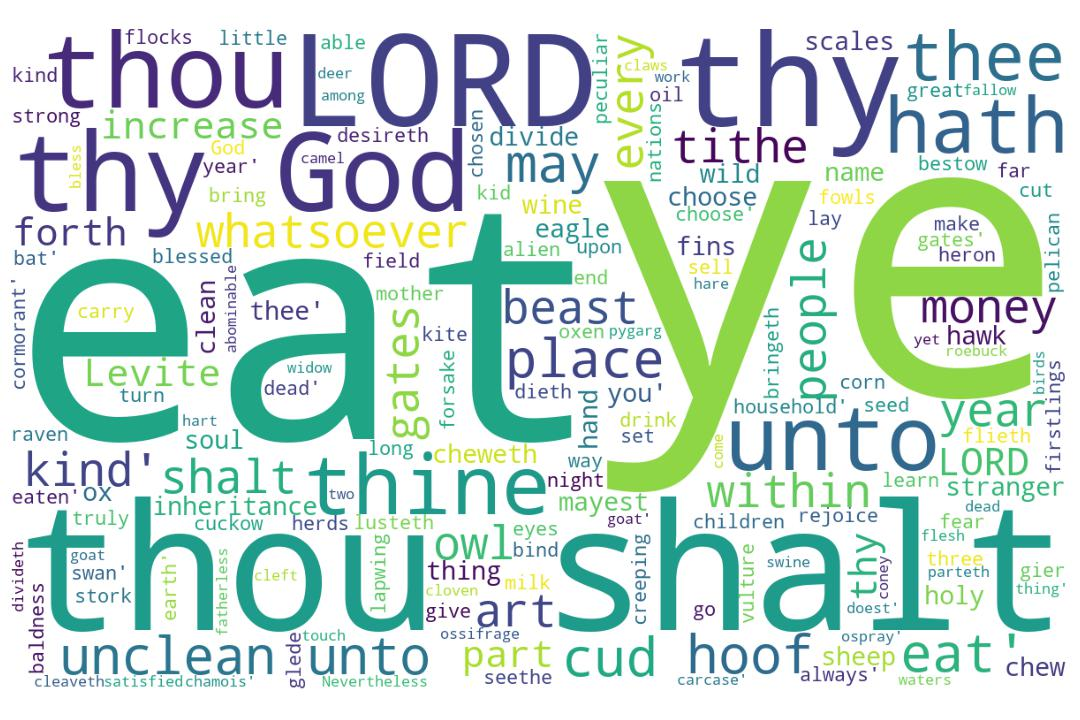
\includegraphics[width=\linewidth]{05OT-Deuteronomy/Deuteronomy14-WordCloud.jpg}
  \caption{Deuteronomy 14 Word Cloud}
  \label{fig:Deuteronomy 14 word Cloud}
\end{figure}

\marginpar{\scriptsize \centering \fcolorbox{bone}{lime}{\textbf{DETAILS}}\\ (Deuteronomy 14:1-29) \begin{compactenum}[I.][8]
    \item  \textbf{Prohibited Foods}  \index[scripture]{Deuteronomy!Deu 14:01--21}(Deu 14:1--21)
    \item  A \textbf{Peculiar People}  \index[scripture]{Deuteronomy!Deu 14:02}(Deu 14:02)
    \item  \textbf{Personal Hygiene}  \index[scripture]{Deuteronomy!Deu 14:08}(Deu 14:08)
    \item  \textbf{Preditory Birds}  \index[scripture]{Deuteronomy!Deu 14:12--19}(Deu 14:12--19)
    \item  \textbf{Prescribed Giving Foods}  \index[scripture]{Deuteronomy!Deu 14:28}(Deu 14:28)
    \item  \textbf{Protective Measures}  %\index[scripture]{Deuteronomy!Deu 14:28}(Deu 14:28)
\end{compactenum}}



\footnote{\textcolor[cmyk]{0.99998,1,0,0}{\hyperlink{TOC}{Return to end of Table of Contents.}}}\footnote{\href{https://audiobible.com/bible/deuteronomy_14.html}{\textcolor[cmyk]{0.99998,1,0,0}{Deuteronomy 14 Audio}}}\textcolor[cmyk]{0.99998,1,0,0}{Ye \emph{are} the children of the LORD your God: ye shall not cut yourselves, nor make any baldness between your eyes for the dead.}
[2] \textcolor[cmyk]{0.99998,1,0,0}{For thou \emph{art} an holy people unto the LORD thy God, and the LORD hath chosen thee to be a \fcolorbox{bone}{lime}{peculiar people} unto himself, above all the nations that \emph{are} upon the earth.}\\
\\
\P \textcolor[cmyk]{0.99998,1,0,0}{Thou \underline{shalt} not eat any \fcolorbox{bone}{lime}{abominable thing}.}
[4] \textcolor[cmyk]{0.99998,1,0,0}{These \emph{are} the beasts which ye shall eat: the ox, the sheep, and the goat,}
[5] \textcolor[cmyk]{0.99998,1,0,0}{The hart, and the roebuck, and the fallow deer, and the wild goat, and the pygarg, and the wild ox, and the chamois.}
[6] \textcolor[cmyk]{0.99998,1,0,0}{And every beast that parteth the hoof, and cleaveth the cleft into two claws, \emph{and} cheweth the cud among the beasts, that ye shall eat.}
[7] \textcolor[cmyk]{0.99998,1,0,0}{Nevertheless these ye shall not eat of them that chew the cud, or of them that divide the cloven hoof; \emph{as} the camel, and the hare, and the coney: for they chew the cud, but divide not the hoof; \emph{therefore} they \emph{are} unclean unto you.}
[8] \textcolor[cmyk]{0.99998,1,0,0}{And the swine, because it divideth the hoof, yet cheweth not the cud, it \emph{is} unclean unto you: ye shall not eat of their flesh, \fcolorbox{bone}{lime}{nor touch} their dead carcase.}\\
\\
\P \textcolor[cmyk]{0.99998,1,0,0}{These ye shall eat of all that \emph{are} in the waters: all that have fins and scales shall ye eat:}
[10] \textcolor[cmyk]{0.99998,1,0,0}{And whatsoever hath not fins and scales ye may not eat; it \emph{is} unclean unto you.}\\
\\
\P \textcolor[cmyk]{0.99998,1,0,0}{\emph{Of} all clean birds ye shall eat.}
[12] \textcolor[cmyk]{0.99998,1,0,0}{But these \emph{are} \emph{they} of which ye shall not eat: the \fcolorbox{bone}{lime}{eagle}, and the \fcolorbox{bone}{lime}{ossifrage}, and the \fcolorbox{bone}{lime}{ospray},}
[13] \textcolor[cmyk]{0.99998,1,0,0}{And the glede, and the kite, and the vulture after his kind,}
[14] \textcolor[cmyk]{0.99998,1,0,0}{And every raven after his kind,}
[15] \textcolor[cmyk]{0.99998,1,0,0}{And the owl, and the night hawk, and the cuckow, and the hawk after his kind,}
[16] \textcolor[cmyk]{0.99998,1,0,0}{The little owl, and the great owl, and the swan,}
[17] \textcolor[cmyk]{0.99998,1,0,0}{And the pelican, and the gier eagle, and the cormorant,}
[18] \textcolor[cmyk]{0.99998,1,0,0}{And the stork, and the heron after her kind, and the lapwing, and the bat.}
[19] \textcolor[cmyk]{0.99998,1,0,0}{And every creeping thing that flieth \emph{is} unclean unto you: they shall not be eaten.}
[20] \textcolor[cmyk]{0.99998,1,0,0}{\emph{But} \emph{of} all clean fowls ye may eat.}\\
\\
\P \textcolor[cmyk]{0.99998,1,0,0}{Ye shall not eat \emph{of} any thing that dieth of itself: thou \underline{shalt} give it unto the stranger that \emph{is} in thy gates, that he may eat it; or thou mayest sell it unto an alien: for thou \emph{art} an holy people unto the LORD thy God. Thou \underline{shalt} not seethe a kid in his mother's milk.}
[22] \textcolor[cmyk]{0.99998,1,0,0}{Thou \underline{shalt} truly tithe all the increase of thy seed, that the field bringeth forth year by year.}
[23] \textcolor[cmyk]{0.99998,1,0,0}{And thou \underline{shalt} eat before the LORD thy God, in the place which he shall choose to place his name there, the tithe of thy corn, of thy wine, and of thine oil, and the firstlings of thy herds and of thy flocks; that thou mayest learn to fear the LORD thy God always.}
[24] \textcolor[cmyk]{0.99998,1,0,0}{And if the way be too long for thee, so that thou art not able to carry it; \emph{or} if the place be too far from thee, which the LORD thy God shall choose to set his name there, when the LORD thy God hath blessed thee:}
[25] \textcolor[cmyk]{0.99998,1,0,0}{Then \underline{shalt} thou turn \emph{it} into money, and bind up the money in thine hand, and \underline{shalt} go unto the place which the LORD thy God shall choose:}
[26] \textcolor[cmyk]{0.99998,1,0,0}{And thou \underline{shalt} bestow that money for whatsoever thy soul lusteth after, for oxen, or for sheep, or for wine, or for strong drink, or for whatsoever thy soul desireth: and thou \underline{shalt} eat there before the LORD thy God, and thou \underline{shalt} rejoice, thou, and thine household,}
[27] \textcolor[cmyk]{0.99998,1,0,0}{And the Levite that \emph{is} within thy gates; thou \underline{shalt} not forsake him; for he hath no part nor inheritance with thee.}\\
\\
\P \textcolor[cmyk]{0.99998,1,0,0}{At the end of three years thou \underline{shalt} \fcolorbox{bone}{lime}{bring forth} all the tithe of thine increase the same year, and \underline{shalt} lay \emph{it} up within thy gates:}
[29] \textcolor[cmyk]{0.99998,1,0,0}{And the Levite, (because he hath no part nor inheritance with thee,) and the stranger, and the fatherless, and the widow, which \emph{are} within thy gates, shall come, and shall eat and be satisfied; that the LORD thy God may bless thee in all the work of thine hand which thou doest.}
\index[NWIV]{24!Deuteronomy!Deu 14:1}\index[AWIP]{Ye!Deuteronomy!Deu 14:1}\index[AWIP]{\emph{are}!Deuteronomy!Deu 14:1}\index[AWIP]{the!Deuteronomy!Deu 14:1}\index[AWIP]{the!Deuteronomy!Deu 14:1 (2)}\index[AWIP]{the!Deuteronomy!Deu 14:1 (3)}\index[AWIP]{children!Deuteronomy!Deu 14:1}\index[AWIP]{of!Deuteronomy!Deu 14:1}\index[AWIP]{LORD!Deuteronomy!Deu 14:1}\index[AWIP]{your!Deuteronomy!Deu 14:1}\index[AWIP]{your!Deuteronomy!Deu 14:1 (2)}\index[AWIP]{God!Deuteronomy!Deu 14:1}\index[AWIP]{ye!Deuteronomy!Deu 14:1}\index[AWIP]{shall!Deuteronomy!Deu 14:1}\index[AWIP]{not!Deuteronomy!Deu 14:1}\index[AWIP]{cut!Deuteronomy!Deu 14:1}\index[AWIP]{yourselves!Deuteronomy!Deu 14:1}\index[AWIP]{nor!Deuteronomy!Deu 14:1}\index[AWIP]{make!Deuteronomy!Deu 14:1}\index[AWIP]{any!Deuteronomy!Deu 14:1}\index[AWIP]{baldness!Deuteronomy!Deu 14:1}\index[AWIP]{between!Deuteronomy!Deu 14:1}\index[AWIP]{eyes!Deuteronomy!Deu 14:1}\index[AWIP]{for!Deuteronomy!Deu 14:1}\index[AWIP]{dead!Deuteronomy!Deu 14:1}\index[AWIP]{\emph{are}!Deuteronomy!Deu 14:1}

\index[NWIV]{33!Deuteronomy!Deu 14:2}\index[AWIP]{For!Deuteronomy!Deu 14:2}\index[AWIP]{thou!Deuteronomy!Deu 14:2}\index[AWIP]{\emph{art}!Deuteronomy!Deu 14:2}\index[AWIP]{an!Deuteronomy!Deu 14:2}\index[AWIP]{holy!Deuteronomy!Deu 14:2}\index[AWIP]{people!Deuteronomy!Deu 14:2}\index[AWIP]{people!Deuteronomy!Deu 14:2 (2)}\index[AWIP]{unto!Deuteronomy!Deu 14:2}\index[AWIP]{unto!Deuteronomy!Deu 14:2 (2)}\index[AWIP]{the!Deuteronomy!Deu 14:2}\index[AWIP]{the!Deuteronomy!Deu 14:2 (2)}\index[AWIP]{the!Deuteronomy!Deu 14:2 (3)}\index[AWIP]{the!Deuteronomy!Deu 14:2 (4)}\index[AWIP]{LORD!Deuteronomy!Deu 14:2}\index[AWIP]{LORD!Deuteronomy!Deu 14:2 (2)}\index[AWIP]{thy!Deuteronomy!Deu 14:2}\index[AWIP]{God!Deuteronomy!Deu 14:2}\index[AWIP]{and!Deuteronomy!Deu 14:2}\index[AWIP]{hath!Deuteronomy!Deu 14:2}\index[AWIP]{chosen!Deuteronomy!Deu 14:2}\index[AWIP]{thee!Deuteronomy!Deu 14:2}\index[AWIP]{to!Deuteronomy!Deu 14:2}\index[AWIP]{be!Deuteronomy!Deu 14:2}\index[AWIP]{a!Deuteronomy!Deu 14:2}\index[AWIP]{peculiar!Deuteronomy!Deu 14:2}\index[AWIP]{himself!Deuteronomy!Deu 14:2}\index[AWIP]{above!Deuteronomy!Deu 14:2}\index[AWIP]{all!Deuteronomy!Deu 14:2}\index[AWIP]{nations!Deuteronomy!Deu 14:2}\index[AWIP]{that!Deuteronomy!Deu 14:2}\index[AWIP]{\emph{are}!Deuteronomy!Deu 14:2}\index[AWIP]{upon!Deuteronomy!Deu 14:2}\index[AWIP]{earth!Deuteronomy!Deu 14:2}\index[AWIP]{\emph{art}!Deuteronomy!Deu 14:2}\index[AWIP]{\emph{are}!Deuteronomy!Deu 14:2}

\index[NWIV]{7!Deuteronomy!Deu 14:3}\index[AWIP]{Thou!Deuteronomy!Deu 14:3}\index[AWIP]{shalt!Deuteronomy!Deu 14:3}\index[AWIP]{not!Deuteronomy!Deu 14:3}\index[AWIP]{eat!Deuteronomy!Deu 14:3}\index[AWIP]{any!Deuteronomy!Deu 14:3}\index[AWIP]{abominable!Deuteronomy!Deu 14:3}\index[AWIP]{thing!Deuteronomy!Deu 14:3}

\index[NWIV]{15!Deuteronomy!Deu 14:4}\index[AWIP]{These!Deuteronomy!Deu 14:4}\index[AWIP]{\emph{are}!Deuteronomy!Deu 14:4}\index[AWIP]{the!Deuteronomy!Deu 14:4}\index[AWIP]{the!Deuteronomy!Deu 14:4 (2)}\index[AWIP]{the!Deuteronomy!Deu 14:4 (3)}\index[AWIP]{the!Deuteronomy!Deu 14:4 (4)}\index[AWIP]{beasts!Deuteronomy!Deu 14:4}\index[AWIP]{which!Deuteronomy!Deu 14:4}\index[AWIP]{ye!Deuteronomy!Deu 14:4}\index[AWIP]{shall!Deuteronomy!Deu 14:4}\index[AWIP]{eat!Deuteronomy!Deu 14:4}\index[AWIP]{ox!Deuteronomy!Deu 14:4}\index[AWIP]{sheep!Deuteronomy!Deu 14:4}\index[AWIP]{and!Deuteronomy!Deu 14:4}\index[AWIP]{goat!Deuteronomy!Deu 14:4}\index[AWIP]{\emph{are}!Deuteronomy!Deu 14:4}

\index[NWIV]{23!Deuteronomy!Deu 14:5}\index[AWIP]{The!Deuteronomy!Deu 14:5}\index[AWIP]{hart!Deuteronomy!Deu 14:5}\index[AWIP]{and!Deuteronomy!Deu 14:5}\index[AWIP]{and!Deuteronomy!Deu 14:5 (2)}\index[AWIP]{and!Deuteronomy!Deu 14:5 (3)}\index[AWIP]{and!Deuteronomy!Deu 14:5 (4)}\index[AWIP]{and!Deuteronomy!Deu 14:5 (5)}\index[AWIP]{and!Deuteronomy!Deu 14:5 (6)}\index[AWIP]{the!Deuteronomy!Deu 14:5}\index[AWIP]{the!Deuteronomy!Deu 14:5 (2)}\index[AWIP]{the!Deuteronomy!Deu 14:5 (3)}\index[AWIP]{the!Deuteronomy!Deu 14:5 (4)}\index[AWIP]{the!Deuteronomy!Deu 14:5 (5)}\index[AWIP]{the!Deuteronomy!Deu 14:5 (6)}\index[AWIP]{roebuck!Deuteronomy!Deu 14:5}\index[AWIP]{fallow!Deuteronomy!Deu 14:5}\index[AWIP]{deer!Deuteronomy!Deu 14:5}\index[AWIP]{wild!Deuteronomy!Deu 14:5}\index[AWIP]{wild!Deuteronomy!Deu 14:5 (2)}\index[AWIP]{goat!Deuteronomy!Deu 14:5}\index[AWIP]{pygarg!Deuteronomy!Deu 14:5}\index[AWIP]{ox!Deuteronomy!Deu 14:5}\index[AWIP]{chamois!Deuteronomy!Deu 14:5}

\index[NWIV]{25!Deuteronomy!Deu 14:6}\index[AWIP]{And!Deuteronomy!Deu 14:6}\index[AWIP]{every!Deuteronomy!Deu 14:6}\index[AWIP]{beast!Deuteronomy!Deu 14:6}\index[AWIP]{that!Deuteronomy!Deu 14:6}\index[AWIP]{that!Deuteronomy!Deu 14:6 (2)}\index[AWIP]{parteth!Deuteronomy!Deu 14:6}\index[AWIP]{the!Deuteronomy!Deu 14:6}\index[AWIP]{the!Deuteronomy!Deu 14:6 (2)}\index[AWIP]{the!Deuteronomy!Deu 14:6 (3)}\index[AWIP]{the!Deuteronomy!Deu 14:6 (4)}\index[AWIP]{hoof!Deuteronomy!Deu 14:6}\index[AWIP]{and!Deuteronomy!Deu 14:6}\index[AWIP]{cleaveth!Deuteronomy!Deu 14:6}\index[AWIP]{cleft!Deuteronomy!Deu 14:6}\index[AWIP]{into!Deuteronomy!Deu 14:6}\index[AWIP]{two!Deuteronomy!Deu 14:6}\index[AWIP]{claws!Deuteronomy!Deu 14:6}\index[AWIP]{\emph{and}!Deuteronomy!Deu 14:6}\index[AWIP]{cheweth!Deuteronomy!Deu 14:6}\index[AWIP]{cud!Deuteronomy!Deu 14:6}\index[AWIP]{among!Deuteronomy!Deu 14:6}\index[AWIP]{beasts!Deuteronomy!Deu 14:6}\index[AWIP]{ye!Deuteronomy!Deu 14:6}\index[AWIP]{shall!Deuteronomy!Deu 14:6}\index[AWIP]{eat!Deuteronomy!Deu 14:6}\index[AWIP]{\emph{and}!Deuteronomy!Deu 14:6}

\index[NWIV]{45!Deuteronomy!Deu 14:7}\index[AWIP]{Nevertheless!Deuteronomy!Deu 14:7}\index[AWIP]{these!Deuteronomy!Deu 14:7}\index[AWIP]{ye!Deuteronomy!Deu 14:7}\index[AWIP]{shall!Deuteronomy!Deu 14:7}\index[AWIP]{not!Deuteronomy!Deu 14:7}\index[AWIP]{not!Deuteronomy!Deu 14:7 (2)}\index[AWIP]{eat!Deuteronomy!Deu 14:7}\index[AWIP]{of!Deuteronomy!Deu 14:7}\index[AWIP]{of!Deuteronomy!Deu 14:7 (2)}\index[AWIP]{them!Deuteronomy!Deu 14:7}\index[AWIP]{them!Deuteronomy!Deu 14:7 (2)}\index[AWIP]{that!Deuteronomy!Deu 14:7}\index[AWIP]{that!Deuteronomy!Deu 14:7 (2)}\index[AWIP]{chew!Deuteronomy!Deu 14:7}\index[AWIP]{chew!Deuteronomy!Deu 14:7 (2)}\index[AWIP]{the!Deuteronomy!Deu 14:7}\index[AWIP]{the!Deuteronomy!Deu 14:7 (2)}\index[AWIP]{the!Deuteronomy!Deu 14:7 (3)}\index[AWIP]{the!Deuteronomy!Deu 14:7 (4)}\index[AWIP]{the!Deuteronomy!Deu 14:7 (5)}\index[AWIP]{the!Deuteronomy!Deu 14:7 (6)}\index[AWIP]{the!Deuteronomy!Deu 14:7 (7)}\index[AWIP]{cud!Deuteronomy!Deu 14:7}\index[AWIP]{cud!Deuteronomy!Deu 14:7 (2)}\index[AWIP]{or!Deuteronomy!Deu 14:7}\index[AWIP]{divide!Deuteronomy!Deu 14:7}\index[AWIP]{divide!Deuteronomy!Deu 14:7 (2)}\index[AWIP]{cloven!Deuteronomy!Deu 14:7}\index[AWIP]{hoof!Deuteronomy!Deu 14:7}\index[AWIP]{hoof!Deuteronomy!Deu 14:7 (2)}\index[AWIP]{\emph{as}!Deuteronomy!Deu 14:7}\index[AWIP]{camel!Deuteronomy!Deu 14:7}\index[AWIP]{and!Deuteronomy!Deu 14:7}\index[AWIP]{and!Deuteronomy!Deu 14:7 (2)}\index[AWIP]{hare!Deuteronomy!Deu 14:7}\index[AWIP]{coney!Deuteronomy!Deu 14:7}\index[AWIP]{for!Deuteronomy!Deu 14:7}\index[AWIP]{they!Deuteronomy!Deu 14:7}\index[AWIP]{they!Deuteronomy!Deu 14:7 (2)}\index[AWIP]{but!Deuteronomy!Deu 14:7}\index[AWIP]{\emph{therefore}!Deuteronomy!Deu 14:7}\index[AWIP]{\emph{are}!Deuteronomy!Deu 14:7}\index[AWIP]{unclean!Deuteronomy!Deu 14:7}\index[AWIP]{unto!Deuteronomy!Deu 14:7}\index[AWIP]{you!Deuteronomy!Deu 14:7}\index[AWIP]{\emph{as}!Deuteronomy!Deu 14:7}\index[AWIP]{\emph{therefore}!Deuteronomy!Deu 14:7}\index[AWIP]{\emph{are}!Deuteronomy!Deu 14:7}

\index[NWIV]{30!Deuteronomy!Deu 14:8}\index[AWIP]{And!Deuteronomy!Deu 14:8}\index[AWIP]{the!Deuteronomy!Deu 14:8}\index[AWIP]{the!Deuteronomy!Deu 14:8 (2)}\index[AWIP]{the!Deuteronomy!Deu 14:8 (3)}\index[AWIP]{swine!Deuteronomy!Deu 14:8}\index[AWIP]{because!Deuteronomy!Deu 14:8}\index[AWIP]{it!Deuteronomy!Deu 14:8}\index[AWIP]{it!Deuteronomy!Deu 14:8 (2)}\index[AWIP]{divideth!Deuteronomy!Deu 14:8}\index[AWIP]{hoof!Deuteronomy!Deu 14:8}\index[AWIP]{yet!Deuteronomy!Deu 14:8}\index[AWIP]{cheweth!Deuteronomy!Deu 14:8}\index[AWIP]{not!Deuteronomy!Deu 14:8}\index[AWIP]{not!Deuteronomy!Deu 14:8 (2)}\index[AWIP]{cud!Deuteronomy!Deu 14:8}\index[AWIP]{\emph{is}!Deuteronomy!Deu 14:8}\index[AWIP]{unclean!Deuteronomy!Deu 14:8}\index[AWIP]{unto!Deuteronomy!Deu 14:8}\index[AWIP]{you!Deuteronomy!Deu 14:8}\index[AWIP]{ye!Deuteronomy!Deu 14:8}\index[AWIP]{shall!Deuteronomy!Deu 14:8}\index[AWIP]{eat!Deuteronomy!Deu 14:8}\index[AWIP]{of!Deuteronomy!Deu 14:8}\index[AWIP]{their!Deuteronomy!Deu 14:8}\index[AWIP]{their!Deuteronomy!Deu 14:8 (2)}\index[AWIP]{flesh!Deuteronomy!Deu 14:8}\index[AWIP]{nor!Deuteronomy!Deu 14:8}\index[AWIP]{touch!Deuteronomy!Deu 14:8}\index[AWIP]{dead!Deuteronomy!Deu 14:8}\index[AWIP]{carcase!Deuteronomy!Deu 14:8}\index[AWIP]{\emph{is}!Deuteronomy!Deu 14:8}

\index[NWIV]{20!Deuteronomy!Deu 14:9}\index[AWIP]{These!Deuteronomy!Deu 14:9}\index[AWIP]{ye!Deuteronomy!Deu 14:9}\index[AWIP]{ye!Deuteronomy!Deu 14:9 (2)}\index[AWIP]{shall!Deuteronomy!Deu 14:9}\index[AWIP]{shall!Deuteronomy!Deu 14:9 (2)}\index[AWIP]{eat!Deuteronomy!Deu 14:9}\index[AWIP]{eat!Deuteronomy!Deu 14:9 (2)}\index[AWIP]{of!Deuteronomy!Deu 14:9}\index[AWIP]{all!Deuteronomy!Deu 14:9}\index[AWIP]{all!Deuteronomy!Deu 14:9 (2)}\index[AWIP]{that!Deuteronomy!Deu 14:9}\index[AWIP]{that!Deuteronomy!Deu 14:9 (2)}\index[AWIP]{\emph{are}!Deuteronomy!Deu 14:9}\index[AWIP]{in!Deuteronomy!Deu 14:9}\index[AWIP]{the!Deuteronomy!Deu 14:9}\index[AWIP]{waters!Deuteronomy!Deu 14:9}\index[AWIP]{have!Deuteronomy!Deu 14:9}\index[AWIP]{fins!Deuteronomy!Deu 14:9}\index[AWIP]{and!Deuteronomy!Deu 14:9}\index[AWIP]{scales!Deuteronomy!Deu 14:9}\index[AWIP]{\emph{are}!Deuteronomy!Deu 14:9}

\index[NWIV]{16!Deuteronomy!Deu 14:10}\index[AWIP]{And!Deuteronomy!Deu 14:10}\index[AWIP]{whatsoever!Deuteronomy!Deu 14:10}\index[AWIP]{hath!Deuteronomy!Deu 14:10}\index[AWIP]{not!Deuteronomy!Deu 14:10}\index[AWIP]{not!Deuteronomy!Deu 14:10 (2)}\index[AWIP]{fins!Deuteronomy!Deu 14:10}\index[AWIP]{and!Deuteronomy!Deu 14:10}\index[AWIP]{scales!Deuteronomy!Deu 14:10}\index[AWIP]{ye!Deuteronomy!Deu 14:10}\index[AWIP]{may!Deuteronomy!Deu 14:10}\index[AWIP]{eat!Deuteronomy!Deu 14:10}\index[AWIP]{it!Deuteronomy!Deu 14:10}\index[AWIP]{\emph{is}!Deuteronomy!Deu 14:10}\index[AWIP]{unclean!Deuteronomy!Deu 14:10}\index[AWIP]{unto!Deuteronomy!Deu 14:10}\index[AWIP]{you!Deuteronomy!Deu 14:10}\index[AWIP]{\emph{is}!Deuteronomy!Deu 14:10}

\index[NWIV]{7!Deuteronomy!Deu 14:11}\index[AWIP]{\emph{Of}!Deuteronomy!Deu 14:11}\index[AWIP]{all!Deuteronomy!Deu 14:11}\index[AWIP]{clean!Deuteronomy!Deu 14:11}\index[AWIP]{birds!Deuteronomy!Deu 14:11}\index[AWIP]{ye!Deuteronomy!Deu 14:11}\index[AWIP]{shall!Deuteronomy!Deu 14:11}\index[AWIP]{eat!Deuteronomy!Deu 14:11}\index[AWIP]{\emph{Of}!Deuteronomy!Deu 14:11}

\index[NWIV]{18!Deuteronomy!Deu 14:12}\index[AWIP]{But!Deuteronomy!Deu 14:12}\index[AWIP]{these!Deuteronomy!Deu 14:12}\index[AWIP]{\emph{are}!Deuteronomy!Deu 14:12}\index[AWIP]{\emph{they}!Deuteronomy!Deu 14:12}\index[AWIP]{of!Deuteronomy!Deu 14:12}\index[AWIP]{which!Deuteronomy!Deu 14:12}\index[AWIP]{ye!Deuteronomy!Deu 14:12}\index[AWIP]{shall!Deuteronomy!Deu 14:12}\index[AWIP]{not!Deuteronomy!Deu 14:12}\index[AWIP]{eat!Deuteronomy!Deu 14:12}\index[AWIP]{the!Deuteronomy!Deu 14:12}\index[AWIP]{the!Deuteronomy!Deu 14:12 (2)}\index[AWIP]{the!Deuteronomy!Deu 14:12 (3)}\index[AWIP]{eagle!Deuteronomy!Deu 14:12}\index[AWIP]{and!Deuteronomy!Deu 14:12}\index[AWIP]{and!Deuteronomy!Deu 14:12 (2)}\index[AWIP]{ossifrage!Deuteronomy!Deu 14:12}\index[AWIP]{ospray!Deuteronomy!Deu 14:12}\index[AWIP]{\emph{are}!Deuteronomy!Deu 14:12}\index[AWIP]{\emph{they}!Deuteronomy!Deu 14:12}

\index[NWIV]{12!Deuteronomy!Deu 14:13}\index[AWIP]{And!Deuteronomy!Deu 14:13}\index[AWIP]{the!Deuteronomy!Deu 14:13}\index[AWIP]{the!Deuteronomy!Deu 14:13 (2)}\index[AWIP]{the!Deuteronomy!Deu 14:13 (3)}\index[AWIP]{glede!Deuteronomy!Deu 14:13}\index[AWIP]{and!Deuteronomy!Deu 14:13}\index[AWIP]{and!Deuteronomy!Deu 14:13 (2)}\index[AWIP]{kite!Deuteronomy!Deu 14:13}\index[AWIP]{vulture!Deuteronomy!Deu 14:13}\index[AWIP]{after!Deuteronomy!Deu 14:13}\index[AWIP]{his!Deuteronomy!Deu 14:13}\index[AWIP]{kind!Deuteronomy!Deu 14:13}

\index[NWIV]{6!Deuteronomy!Deu 14:14}\index[AWIP]{And!Deuteronomy!Deu 14:14}\index[AWIP]{every!Deuteronomy!Deu 14:14}\index[AWIP]{raven!Deuteronomy!Deu 14:14}\index[AWIP]{after!Deuteronomy!Deu 14:14}\index[AWIP]{his!Deuteronomy!Deu 14:14}\index[AWIP]{kind!Deuteronomy!Deu 14:14}

\index[NWIV]{16!Deuteronomy!Deu 14:15}\index[AWIP]{And!Deuteronomy!Deu 14:15}\index[AWIP]{the!Deuteronomy!Deu 14:15}\index[AWIP]{the!Deuteronomy!Deu 14:15 (2)}\index[AWIP]{the!Deuteronomy!Deu 14:15 (3)}\index[AWIP]{the!Deuteronomy!Deu 14:15 (4)}\index[AWIP]{owl!Deuteronomy!Deu 14:15}\index[AWIP]{and!Deuteronomy!Deu 14:15}\index[AWIP]{and!Deuteronomy!Deu 14:15 (2)}\index[AWIP]{and!Deuteronomy!Deu 14:15 (3)}\index[AWIP]{night!Deuteronomy!Deu 14:15}\index[AWIP]{hawk!Deuteronomy!Deu 14:15}\index[AWIP]{hawk!Deuteronomy!Deu 14:15 (2)}\index[AWIP]{cuckow!Deuteronomy!Deu 14:15}\index[AWIP]{after!Deuteronomy!Deu 14:15}\index[AWIP]{his!Deuteronomy!Deu 14:15}\index[AWIP]{kind!Deuteronomy!Deu 14:15}

\index[NWIV]{10!Deuteronomy!Deu 14:16}\index[AWIP]{The!Deuteronomy!Deu 14:16}\index[AWIP]{little!Deuteronomy!Deu 14:16}\index[AWIP]{owl!Deuteronomy!Deu 14:16}\index[AWIP]{owl!Deuteronomy!Deu 14:16 (2)}\index[AWIP]{and!Deuteronomy!Deu 14:16}\index[AWIP]{and!Deuteronomy!Deu 14:16 (2)}\index[AWIP]{the!Deuteronomy!Deu 14:16}\index[AWIP]{the!Deuteronomy!Deu 14:16 (2)}\index[AWIP]{great!Deuteronomy!Deu 14:16}\index[AWIP]{swan!Deuteronomy!Deu 14:16}

\index[NWIV]{10!Deuteronomy!Deu 14:17}\index[AWIP]{And!Deuteronomy!Deu 14:17}\index[AWIP]{the!Deuteronomy!Deu 14:17}\index[AWIP]{the!Deuteronomy!Deu 14:17 (2)}\index[AWIP]{the!Deuteronomy!Deu 14:17 (3)}\index[AWIP]{pelican!Deuteronomy!Deu 14:17}\index[AWIP]{and!Deuteronomy!Deu 14:17}\index[AWIP]{and!Deuteronomy!Deu 14:17 (2)}\index[AWIP]{gier!Deuteronomy!Deu 14:17}\index[AWIP]{eagle!Deuteronomy!Deu 14:17}\index[AWIP]{cormorant!Deuteronomy!Deu 14:17}

\index[NWIV]{15!Deuteronomy!Deu 14:18}\index[AWIP]{And!Deuteronomy!Deu 14:18}\index[AWIP]{the!Deuteronomy!Deu 14:18}\index[AWIP]{the!Deuteronomy!Deu 14:18 (2)}\index[AWIP]{the!Deuteronomy!Deu 14:18 (3)}\index[AWIP]{the!Deuteronomy!Deu 14:18 (4)}\index[AWIP]{stork!Deuteronomy!Deu 14:18}\index[AWIP]{and!Deuteronomy!Deu 14:18}\index[AWIP]{and!Deuteronomy!Deu 14:18 (2)}\index[AWIP]{and!Deuteronomy!Deu 14:18 (3)}\index[AWIP]{heron!Deuteronomy!Deu 14:18}\index[AWIP]{after!Deuteronomy!Deu 14:18}\index[AWIP]{her!Deuteronomy!Deu 14:18}\index[AWIP]{kind!Deuteronomy!Deu 14:18}\index[AWIP]{lapwing!Deuteronomy!Deu 14:18}\index[AWIP]{bat!Deuteronomy!Deu 14:18}

\index[NWIV]{15!Deuteronomy!Deu 14:19}\index[AWIP]{And!Deuteronomy!Deu 14:19}\index[AWIP]{every!Deuteronomy!Deu 14:19}\index[AWIP]{creeping!Deuteronomy!Deu 14:19}\index[AWIP]{thing!Deuteronomy!Deu 14:19}\index[AWIP]{that!Deuteronomy!Deu 14:19}\index[AWIP]{flieth!Deuteronomy!Deu 14:19}\index[AWIP]{\emph{is}!Deuteronomy!Deu 14:19}\index[AWIP]{unclean!Deuteronomy!Deu 14:19}\index[AWIP]{unto!Deuteronomy!Deu 14:19}\index[AWIP]{you!Deuteronomy!Deu 14:19}\index[AWIP]{they!Deuteronomy!Deu 14:19}\index[AWIP]{shall!Deuteronomy!Deu 14:19}\index[AWIP]{not!Deuteronomy!Deu 14:19}\index[AWIP]{be!Deuteronomy!Deu 14:19}\index[AWIP]{eaten!Deuteronomy!Deu 14:19}\index[AWIP]{\emph{is}!Deuteronomy!Deu 14:19}

\index[NWIV]{8!Deuteronomy!Deu 14:20}\index[AWIP]{\emph{But}!Deuteronomy!Deu 14:20}\index[AWIP]{\emph{of}!Deuteronomy!Deu 14:20}\index[AWIP]{all!Deuteronomy!Deu 14:20}\index[AWIP]{clean!Deuteronomy!Deu 14:20}\index[AWIP]{fowls!Deuteronomy!Deu 14:20}\index[AWIP]{ye!Deuteronomy!Deu 14:20}\index[AWIP]{may!Deuteronomy!Deu 14:20}\index[AWIP]{eat!Deuteronomy!Deu 14:20}\index[AWIP]{\emph{But}!Deuteronomy!Deu 14:20}\index[AWIP]{\emph{of}!Deuteronomy!Deu 14:20}

\index[NWIV]{57!Deuteronomy!Deu 14:21}\index[AWIP]{Ye!Deuteronomy!Deu 14:21}\index[AWIP]{shall!Deuteronomy!Deu 14:21}\index[AWIP]{not!Deuteronomy!Deu 14:21}\index[AWIP]{not!Deuteronomy!Deu 14:21 (2)}\index[AWIP]{eat!Deuteronomy!Deu 14:21}\index[AWIP]{eat!Deuteronomy!Deu 14:21 (2)}\index[AWIP]{\emph{of}!Deuteronomy!Deu 14:21}\index[AWIP]{any!Deuteronomy!Deu 14:21}\index[AWIP]{thing!Deuteronomy!Deu 14:21}\index[AWIP]{that!Deuteronomy!Deu 14:21}\index[AWIP]{that!Deuteronomy!Deu 14:21 (2)}\index[AWIP]{that!Deuteronomy!Deu 14:21 (3)}\index[AWIP]{dieth!Deuteronomy!Deu 14:21}\index[AWIP]{of!Deuteronomy!Deu 14:21}\index[AWIP]{itself!Deuteronomy!Deu 14:21}\index[AWIP]{thou!Deuteronomy!Deu 14:21}\index[AWIP]{thou!Deuteronomy!Deu 14:21 (2)}\index[AWIP]{thou!Deuteronomy!Deu 14:21 (3)}\index[AWIP]{shalt!Deuteronomy!Deu 14:21}\index[AWIP]{shalt!Deuteronomy!Deu 14:21 (2)}\index[AWIP]{give!Deuteronomy!Deu 14:21}\index[AWIP]{it!Deuteronomy!Deu 14:21}\index[AWIP]{it!Deuteronomy!Deu 14:21 (2)}\index[AWIP]{it!Deuteronomy!Deu 14:21 (3)}\index[AWIP]{unto!Deuteronomy!Deu 14:21}\index[AWIP]{unto!Deuteronomy!Deu 14:21 (2)}\index[AWIP]{unto!Deuteronomy!Deu 14:21 (3)}\index[AWIP]{the!Deuteronomy!Deu 14:21}\index[AWIP]{the!Deuteronomy!Deu 14:21 (2)}\index[AWIP]{stranger!Deuteronomy!Deu 14:21}\index[AWIP]{\emph{is}!Deuteronomy!Deu 14:21}\index[AWIP]{in!Deuteronomy!Deu 14:21}\index[AWIP]{in!Deuteronomy!Deu 14:21 (2)}\index[AWIP]{thy!Deuteronomy!Deu 14:21}\index[AWIP]{thy!Deuteronomy!Deu 14:21 (2)}\index[AWIP]{gates!Deuteronomy!Deu 14:21}\index[AWIP]{he!Deuteronomy!Deu 14:21}\index[AWIP]{may!Deuteronomy!Deu 14:21}\index[AWIP]{or!Deuteronomy!Deu 14:21}\index[AWIP]{mayest!Deuteronomy!Deu 14:21}\index[AWIP]{sell!Deuteronomy!Deu 14:21}\index[AWIP]{an!Deuteronomy!Deu 14:21}\index[AWIP]{an!Deuteronomy!Deu 14:21 (2)}\index[AWIP]{alien!Deuteronomy!Deu 14:21}\index[AWIP]{for!Deuteronomy!Deu 14:21}\index[AWIP]{\emph{art}!Deuteronomy!Deu 14:21}\index[AWIP]{holy!Deuteronomy!Deu 14:21}\index[AWIP]{people!Deuteronomy!Deu 14:21}\index[AWIP]{LORD!Deuteronomy!Deu 14:21}\index[AWIP]{God!Deuteronomy!Deu 14:21}\index[AWIP]{Thou!Deuteronomy!Deu 14:21}\index[AWIP]{seethe!Deuteronomy!Deu 14:21}\index[AWIP]{a!Deuteronomy!Deu 14:21}\index[AWIP]{kid!Deuteronomy!Deu 14:21}\index[AWIP]{his!Deuteronomy!Deu 14:21}\index[AWIP]{mother's!Deuteronomy!Deu 14:21}\index[AWIP]{milk!Deuteronomy!Deu 14:21}\index[AWIP]{\emph{of}!Deuteronomy!Deu 14:21}\index[AWIP]{\emph{is}!Deuteronomy!Deu 14:21}\index[AWIP]{\emph{art}!Deuteronomy!Deu 14:21}

\index[NWIV]{18!Deuteronomy!Deu 14:22}\index[AWIP]{Thou!Deuteronomy!Deu 14:22}\index[AWIP]{shalt!Deuteronomy!Deu 14:22}\index[AWIP]{truly!Deuteronomy!Deu 14:22}\index[AWIP]{tithe!Deuteronomy!Deu 14:22}\index[AWIP]{all!Deuteronomy!Deu 14:22}\index[AWIP]{the!Deuteronomy!Deu 14:22}\index[AWIP]{the!Deuteronomy!Deu 14:22 (2)}\index[AWIP]{increase!Deuteronomy!Deu 14:22}\index[AWIP]{of!Deuteronomy!Deu 14:22}\index[AWIP]{thy!Deuteronomy!Deu 14:22}\index[AWIP]{seed!Deuteronomy!Deu 14:22}\index[AWIP]{that!Deuteronomy!Deu 14:22}\index[AWIP]{field!Deuteronomy!Deu 14:22}\index[AWIP]{bringeth!Deuteronomy!Deu 14:22}\index[AWIP]{forth!Deuteronomy!Deu 14:22}\index[AWIP]{year!Deuteronomy!Deu 14:22}\index[AWIP]{year!Deuteronomy!Deu 14:22 (2)}\index[AWIP]{by!Deuteronomy!Deu 14:22}

\index[NWIV]{54!Deuteronomy!Deu 14:23}\index[AWIP]{And!Deuteronomy!Deu 14:23}\index[AWIP]{thou!Deuteronomy!Deu 14:23}\index[AWIP]{thou!Deuteronomy!Deu 14:23 (2)}\index[AWIP]{shalt!Deuteronomy!Deu 14:23}\index[AWIP]{eat!Deuteronomy!Deu 14:23}\index[AWIP]{before!Deuteronomy!Deu 14:23}\index[AWIP]{the!Deuteronomy!Deu 14:23}\index[AWIP]{the!Deuteronomy!Deu 14:23 (2)}\index[AWIP]{the!Deuteronomy!Deu 14:23 (3)}\index[AWIP]{the!Deuteronomy!Deu 14:23 (4)}\index[AWIP]{the!Deuteronomy!Deu 14:23 (5)}\index[AWIP]{LORD!Deuteronomy!Deu 14:23}\index[AWIP]{LORD!Deuteronomy!Deu 14:23 (2)}\index[AWIP]{thy!Deuteronomy!Deu 14:23}\index[AWIP]{thy!Deuteronomy!Deu 14:23 (2)}\index[AWIP]{thy!Deuteronomy!Deu 14:23 (3)}\index[AWIP]{thy!Deuteronomy!Deu 14:23 (4)}\index[AWIP]{thy!Deuteronomy!Deu 14:23 (5)}\index[AWIP]{thy!Deuteronomy!Deu 14:23 (6)}\index[AWIP]{God!Deuteronomy!Deu 14:23}\index[AWIP]{God!Deuteronomy!Deu 14:23 (2)}\index[AWIP]{in!Deuteronomy!Deu 14:23}\index[AWIP]{place!Deuteronomy!Deu 14:23}\index[AWIP]{place!Deuteronomy!Deu 14:23 (2)}\index[AWIP]{which!Deuteronomy!Deu 14:23}\index[AWIP]{he!Deuteronomy!Deu 14:23}\index[AWIP]{shall!Deuteronomy!Deu 14:23}\index[AWIP]{choose!Deuteronomy!Deu 14:23}\index[AWIP]{to!Deuteronomy!Deu 14:23}\index[AWIP]{to!Deuteronomy!Deu 14:23 (2)}\index[AWIP]{his!Deuteronomy!Deu 14:23}\index[AWIP]{name!Deuteronomy!Deu 14:23}\index[AWIP]{there!Deuteronomy!Deu 14:23}\index[AWIP]{tithe!Deuteronomy!Deu 14:23}\index[AWIP]{of!Deuteronomy!Deu 14:23}\index[AWIP]{of!Deuteronomy!Deu 14:23 (2)}\index[AWIP]{of!Deuteronomy!Deu 14:23 (3)}\index[AWIP]{of!Deuteronomy!Deu 14:23 (4)}\index[AWIP]{of!Deuteronomy!Deu 14:23 (5)}\index[AWIP]{corn!Deuteronomy!Deu 14:23}\index[AWIP]{wine!Deuteronomy!Deu 14:23}\index[AWIP]{and!Deuteronomy!Deu 14:23}\index[AWIP]{and!Deuteronomy!Deu 14:23 (2)}\index[AWIP]{and!Deuteronomy!Deu 14:23 (3)}\index[AWIP]{thine!Deuteronomy!Deu 14:23}\index[AWIP]{oil!Deuteronomy!Deu 14:23}\index[AWIP]{firstlings!Deuteronomy!Deu 14:23}\index[AWIP]{herds!Deuteronomy!Deu 14:23}\index[AWIP]{flocks!Deuteronomy!Deu 14:23}\index[AWIP]{that!Deuteronomy!Deu 14:23}\index[AWIP]{mayest!Deuteronomy!Deu 14:23}\index[AWIP]{learn!Deuteronomy!Deu 14:23}\index[AWIP]{fear!Deuteronomy!Deu 14:23}\index[AWIP]{always!Deuteronomy!Deu 14:23}

\index[NWIV]{47!Deuteronomy!Deu 14:24}\index[AWIP]{And!Deuteronomy!Deu 14:24}\index[AWIP]{if!Deuteronomy!Deu 14:24}\index[AWIP]{if!Deuteronomy!Deu 14:24 (2)}\index[AWIP]{the!Deuteronomy!Deu 14:24}\index[AWIP]{the!Deuteronomy!Deu 14:24 (2)}\index[AWIP]{the!Deuteronomy!Deu 14:24 (3)}\index[AWIP]{the!Deuteronomy!Deu 14:24 (4)}\index[AWIP]{way!Deuteronomy!Deu 14:24}\index[AWIP]{be!Deuteronomy!Deu 14:24}\index[AWIP]{be!Deuteronomy!Deu 14:24 (2)}\index[AWIP]{too!Deuteronomy!Deu 14:24}\index[AWIP]{too!Deuteronomy!Deu 14:24 (2)}\index[AWIP]{long!Deuteronomy!Deu 14:24}\index[AWIP]{for!Deuteronomy!Deu 14:24}\index[AWIP]{thee!Deuteronomy!Deu 14:24}\index[AWIP]{thee!Deuteronomy!Deu 14:24 (2)}\index[AWIP]{thee!Deuteronomy!Deu 14:24 (3)}\index[AWIP]{so!Deuteronomy!Deu 14:24}\index[AWIP]{that!Deuteronomy!Deu 14:24}\index[AWIP]{thou!Deuteronomy!Deu 14:24}\index[AWIP]{art!Deuteronomy!Deu 14:24}\index[AWIP]{not!Deuteronomy!Deu 14:24}\index[AWIP]{able!Deuteronomy!Deu 14:24}\index[AWIP]{to!Deuteronomy!Deu 14:24}\index[AWIP]{to!Deuteronomy!Deu 14:24 (2)}\index[AWIP]{carry!Deuteronomy!Deu 14:24}\index[AWIP]{it!Deuteronomy!Deu 14:24}\index[AWIP]{\emph{or}!Deuteronomy!Deu 14:24}\index[AWIP]{place!Deuteronomy!Deu 14:24}\index[AWIP]{far!Deuteronomy!Deu 14:24}\index[AWIP]{from!Deuteronomy!Deu 14:24}\index[AWIP]{which!Deuteronomy!Deu 14:24}\index[AWIP]{LORD!Deuteronomy!Deu 14:24}\index[AWIP]{LORD!Deuteronomy!Deu 14:24 (2)}\index[AWIP]{thy!Deuteronomy!Deu 14:24}\index[AWIP]{thy!Deuteronomy!Deu 14:24 (2)}\index[AWIP]{God!Deuteronomy!Deu 14:24}\index[AWIP]{God!Deuteronomy!Deu 14:24 (2)}\index[AWIP]{shall!Deuteronomy!Deu 14:24}\index[AWIP]{choose!Deuteronomy!Deu 14:24}\index[AWIP]{set!Deuteronomy!Deu 14:24}\index[AWIP]{his!Deuteronomy!Deu 14:24}\index[AWIP]{name!Deuteronomy!Deu 14:24}\index[AWIP]{there!Deuteronomy!Deu 14:24}\index[AWIP]{when!Deuteronomy!Deu 14:24}\index[AWIP]{hath!Deuteronomy!Deu 14:24}\index[AWIP]{blessed!Deuteronomy!Deu 14:24}\index[AWIP]{\emph{or}!Deuteronomy!Deu 14:24}

\index[NWIV]{28!Deuteronomy!Deu 14:25}\index[AWIP]{Then!Deuteronomy!Deu 14:25}\index[AWIP]{shalt!Deuteronomy!Deu 14:25}\index[AWIP]{shalt!Deuteronomy!Deu 14:25 (2)}\index[AWIP]{thou!Deuteronomy!Deu 14:25}\index[AWIP]{turn!Deuteronomy!Deu 14:25}\index[AWIP]{\emph{it}!Deuteronomy!Deu 14:25}\index[AWIP]{into!Deuteronomy!Deu 14:25}\index[AWIP]{money!Deuteronomy!Deu 14:25}\index[AWIP]{money!Deuteronomy!Deu 14:25 (2)}\index[AWIP]{and!Deuteronomy!Deu 14:25}\index[AWIP]{and!Deuteronomy!Deu 14:25 (2)}\index[AWIP]{bind!Deuteronomy!Deu 14:25}\index[AWIP]{up!Deuteronomy!Deu 14:25}\index[AWIP]{the!Deuteronomy!Deu 14:25}\index[AWIP]{the!Deuteronomy!Deu 14:25 (2)}\index[AWIP]{the!Deuteronomy!Deu 14:25 (3)}\index[AWIP]{in!Deuteronomy!Deu 14:25}\index[AWIP]{thine!Deuteronomy!Deu 14:25}\index[AWIP]{hand!Deuteronomy!Deu 14:25}\index[AWIP]{go!Deuteronomy!Deu 14:25}\index[AWIP]{unto!Deuteronomy!Deu 14:25}\index[AWIP]{place!Deuteronomy!Deu 14:25}\index[AWIP]{which!Deuteronomy!Deu 14:25}\index[AWIP]{LORD!Deuteronomy!Deu 14:25}\index[AWIP]{thy!Deuteronomy!Deu 14:25}\index[AWIP]{God!Deuteronomy!Deu 14:25}\index[AWIP]{shall!Deuteronomy!Deu 14:25}\index[AWIP]{choose!Deuteronomy!Deu 14:25}\index[AWIP]{\emph{it}!Deuteronomy!Deu 14:25}

\index[NWIV]{48!Deuteronomy!Deu 14:26}\index[AWIP]{And!Deuteronomy!Deu 14:26}\index[AWIP]{thou!Deuteronomy!Deu 14:26}\index[AWIP]{thou!Deuteronomy!Deu 14:26 (2)}\index[AWIP]{thou!Deuteronomy!Deu 14:26 (3)}\index[AWIP]{thou!Deuteronomy!Deu 14:26 (4)}\index[AWIP]{shalt!Deuteronomy!Deu 14:26}\index[AWIP]{shalt!Deuteronomy!Deu 14:26 (2)}\index[AWIP]{shalt!Deuteronomy!Deu 14:26 (3)}\index[AWIP]{bestow!Deuteronomy!Deu 14:26}\index[AWIP]{that!Deuteronomy!Deu 14:26}\index[AWIP]{money!Deuteronomy!Deu 14:26}\index[AWIP]{for!Deuteronomy!Deu 14:26}\index[AWIP]{for!Deuteronomy!Deu 14:26 (2)}\index[AWIP]{for!Deuteronomy!Deu 14:26 (3)}\index[AWIP]{for!Deuteronomy!Deu 14:26 (4)}\index[AWIP]{for!Deuteronomy!Deu 14:26 (5)}\index[AWIP]{for!Deuteronomy!Deu 14:26 (6)}\index[AWIP]{whatsoever!Deuteronomy!Deu 14:26}\index[AWIP]{whatsoever!Deuteronomy!Deu 14:26 (2)}\index[AWIP]{thy!Deuteronomy!Deu 14:26}\index[AWIP]{thy!Deuteronomy!Deu 14:26 (2)}\index[AWIP]{thy!Deuteronomy!Deu 14:26 (3)}\index[AWIP]{soul!Deuteronomy!Deu 14:26}\index[AWIP]{soul!Deuteronomy!Deu 14:26 (2)}\index[AWIP]{lusteth!Deuteronomy!Deu 14:26}\index[AWIP]{after!Deuteronomy!Deu 14:26}\index[AWIP]{oxen!Deuteronomy!Deu 14:26}\index[AWIP]{or!Deuteronomy!Deu 14:26}\index[AWIP]{or!Deuteronomy!Deu 14:26 (2)}\index[AWIP]{or!Deuteronomy!Deu 14:26 (3)}\index[AWIP]{or!Deuteronomy!Deu 14:26 (4)}\index[AWIP]{sheep!Deuteronomy!Deu 14:26}\index[AWIP]{wine!Deuteronomy!Deu 14:26}\index[AWIP]{strong!Deuteronomy!Deu 14:26}\index[AWIP]{drink!Deuteronomy!Deu 14:26}\index[AWIP]{desireth!Deuteronomy!Deu 14:26}\index[AWIP]{and!Deuteronomy!Deu 14:26}\index[AWIP]{and!Deuteronomy!Deu 14:26 (2)}\index[AWIP]{and!Deuteronomy!Deu 14:26 (3)}\index[AWIP]{eat!Deuteronomy!Deu 14:26}\index[AWIP]{there!Deuteronomy!Deu 14:26}\index[AWIP]{before!Deuteronomy!Deu 14:26}\index[AWIP]{the!Deuteronomy!Deu 14:26}\index[AWIP]{LORD!Deuteronomy!Deu 14:26}\index[AWIP]{God!Deuteronomy!Deu 14:26}\index[AWIP]{rejoice!Deuteronomy!Deu 14:26}\index[AWIP]{thine!Deuteronomy!Deu 14:26}\index[AWIP]{household!Deuteronomy!Deu 14:26}

\index[NWIV]{22!Deuteronomy!Deu 14:27}\index[AWIP]{And!Deuteronomy!Deu 14:27}\index[AWIP]{the!Deuteronomy!Deu 14:27}\index[AWIP]{Levite!Deuteronomy!Deu 14:27}\index[AWIP]{that!Deuteronomy!Deu 14:27}\index[AWIP]{\emph{is}!Deuteronomy!Deu 14:27}\index[AWIP]{within!Deuteronomy!Deu 14:27}\index[AWIP]{thy!Deuteronomy!Deu 14:27}\index[AWIP]{gates!Deuteronomy!Deu 14:27}\index[AWIP]{thou!Deuteronomy!Deu 14:27}\index[AWIP]{shalt!Deuteronomy!Deu 14:27}\index[AWIP]{not!Deuteronomy!Deu 14:27}\index[AWIP]{forsake!Deuteronomy!Deu 14:27}\index[AWIP]{him!Deuteronomy!Deu 14:27}\index[AWIP]{for!Deuteronomy!Deu 14:27}\index[AWIP]{he!Deuteronomy!Deu 14:27}\index[AWIP]{hath!Deuteronomy!Deu 14:27}\index[AWIP]{no!Deuteronomy!Deu 14:27}\index[AWIP]{part!Deuteronomy!Deu 14:27}\index[AWIP]{nor!Deuteronomy!Deu 14:27}\index[AWIP]{inheritance!Deuteronomy!Deu 14:27}\index[AWIP]{with!Deuteronomy!Deu 14:27}\index[AWIP]{thee!Deuteronomy!Deu 14:27}\index[AWIP]{\emph{is}!Deuteronomy!Deu 14:27}

\index[NWIV]{27!Deuteronomy!Deu 14:28}\index[AWIP]{At!Deuteronomy!Deu 14:28}\index[AWIP]{the!Deuteronomy!Deu 14:28}\index[AWIP]{the!Deuteronomy!Deu 14:28 (2)}\index[AWIP]{the!Deuteronomy!Deu 14:28 (3)}\index[AWIP]{end!Deuteronomy!Deu 14:28}\index[AWIP]{of!Deuteronomy!Deu 14:28}\index[AWIP]{of!Deuteronomy!Deu 14:28 (2)}\index[AWIP]{three!Deuteronomy!Deu 14:28}\index[AWIP]{years!Deuteronomy!Deu 14:28}\index[AWIP]{thou!Deuteronomy!Deu 14:28}\index[AWIP]{shalt!Deuteronomy!Deu 14:28}\index[AWIP]{shalt!Deuteronomy!Deu 14:28 (2)}\index[AWIP]{bring!Deuteronomy!Deu 14:28}\index[AWIP]{forth!Deuteronomy!Deu 14:28}\index[AWIP]{all!Deuteronomy!Deu 14:28}\index[AWIP]{tithe!Deuteronomy!Deu 14:28}\index[AWIP]{thine!Deuteronomy!Deu 14:28}\index[AWIP]{increase!Deuteronomy!Deu 14:28}\index[AWIP]{same!Deuteronomy!Deu 14:28}\index[AWIP]{year!Deuteronomy!Deu 14:28}\index[AWIP]{and!Deuteronomy!Deu 14:28}\index[AWIP]{lay!Deuteronomy!Deu 14:28}\index[AWIP]{\emph{it}!Deuteronomy!Deu 14:28}\index[AWIP]{up!Deuteronomy!Deu 14:28}\index[AWIP]{within!Deuteronomy!Deu 14:28}\index[AWIP]{thy!Deuteronomy!Deu 14:28}\index[AWIP]{gates!Deuteronomy!Deu 14:28}\index[AWIP]{\emph{it}!Deuteronomy!Deu 14:28}

\index[NWIV]{52!Deuteronomy!Deu 14:29}\index[AWIP]{And!Deuteronomy!Deu 14:29}\index[AWIP]{the!Deuteronomy!Deu 14:29}\index[AWIP]{the!Deuteronomy!Deu 14:29 (2)}\index[AWIP]{the!Deuteronomy!Deu 14:29 (3)}\index[AWIP]{the!Deuteronomy!Deu 14:29 (4)}\index[AWIP]{the!Deuteronomy!Deu 14:29 (5)}\index[AWIP]{the!Deuteronomy!Deu 14:29 (6)}\index[AWIP]{Levite!Deuteronomy!Deu 14:29}\index[AWIP]{(because!Deuteronomy!Deu 14:29}\index[AWIP]{he!Deuteronomy!Deu 14:29}\index[AWIP]{hath!Deuteronomy!Deu 14:29}\index[AWIP]{no!Deuteronomy!Deu 14:29}\index[AWIP]{part!Deuteronomy!Deu 14:29}\index[AWIP]{nor!Deuteronomy!Deu 14:29}\index[AWIP]{inheritance!Deuteronomy!Deu 14:29}\index[AWIP]{with!Deuteronomy!Deu 14:29}\index[AWIP]{thee)!Deuteronomy!Deu 14:29}\index[AWIP]{and!Deuteronomy!Deu 14:29}\index[AWIP]{and!Deuteronomy!Deu 14:29 (2)}\index[AWIP]{and!Deuteronomy!Deu 14:29 (3)}\index[AWIP]{and!Deuteronomy!Deu 14:29 (4)}\index[AWIP]{and!Deuteronomy!Deu 14:29 (5)}\index[AWIP]{stranger!Deuteronomy!Deu 14:29}\index[AWIP]{fatherless!Deuteronomy!Deu 14:29}\index[AWIP]{widow!Deuteronomy!Deu 14:29}\index[AWIP]{which!Deuteronomy!Deu 14:29}\index[AWIP]{which!Deuteronomy!Deu 14:29 (2)}\index[AWIP]{\emph{are}!Deuteronomy!Deu 14:29}\index[AWIP]{within!Deuteronomy!Deu 14:29}\index[AWIP]{thy!Deuteronomy!Deu 14:29}\index[AWIP]{thy!Deuteronomy!Deu 14:29 (2)}\index[AWIP]{gates!Deuteronomy!Deu 14:29}\index[AWIP]{shall!Deuteronomy!Deu 14:29}\index[AWIP]{shall!Deuteronomy!Deu 14:29 (2)}\index[AWIP]{come!Deuteronomy!Deu 14:29}\index[AWIP]{eat!Deuteronomy!Deu 14:29}\index[AWIP]{be!Deuteronomy!Deu 14:29}\index[AWIP]{satisfied!Deuteronomy!Deu 14:29}\index[AWIP]{that!Deuteronomy!Deu 14:29}\index[AWIP]{LORD!Deuteronomy!Deu 14:29}\index[AWIP]{God!Deuteronomy!Deu 14:29}\index[AWIP]{may!Deuteronomy!Deu 14:29}\index[AWIP]{bless!Deuteronomy!Deu 14:29}\index[AWIP]{thee!Deuteronomy!Deu 14:29}\index[AWIP]{in!Deuteronomy!Deu 14:29}\index[AWIP]{all!Deuteronomy!Deu 14:29}\index[AWIP]{work!Deuteronomy!Deu 14:29}\index[AWIP]{of!Deuteronomy!Deu 14:29}\index[AWIP]{thine!Deuteronomy!Deu 14:29}\index[AWIP]{hand!Deuteronomy!Deu 14:29}\index[AWIP]{thou!Deuteronomy!Deu 14:29}\index[AWIP]{doest!Deuteronomy!Deu 14:29}\index[AWIP]{\emph{are}!Deuteronomy!Deu 14:29}


\section{Deuteronomy 14 Outlines}

\subsection{My Outlines}

\subsubsection{Details}
\index[speaker]{Keith Anthony!Deuteronomy 14 (Details)}
\index[series]{Deuteronomy (Keith Anthony)!Deuteronomy 14 (Details)}
\index[date]{2018/02/25!Deuteronomy 14 (Details) (Keith Anthony)}

\begin{compactenum}[I.] 
    \item  \textbf{Prohibited Foods}  \index[scripture]{Deuteronomy!Deu 14:01--21}(Deu 14:1--21)
    \item  A \textbf{Peculiar People}  \index[scripture]{Deuteronomy!Deu 14:02}(Deu 14:02)
    \item  \textbf{Personal Hygiene}  \index[scripture]{Deuteronomy!Deu 14:08}(Deu 14:08)
    \item  \textbf{Preditory Birds}  \index[scripture]{Deuteronomy!Deu 14:12--19}(Deu 14:12--19)
    \item  \textbf{Prescribed Giving Foods}  \index[scripture]{Deuteronomy!Deu 14:28}(Deu 14:28)
    \item  \textbf{Protective Measures}  %\index[scripture]{Deuteronomy!Deu 14:28}(Deu 14:28)
\end{compactenum}
\subsection{My Outlines from Others}


\section{Deuteronomy 14 Comments}



\chapter{Deuteronomy 15}

\begin{figure}
  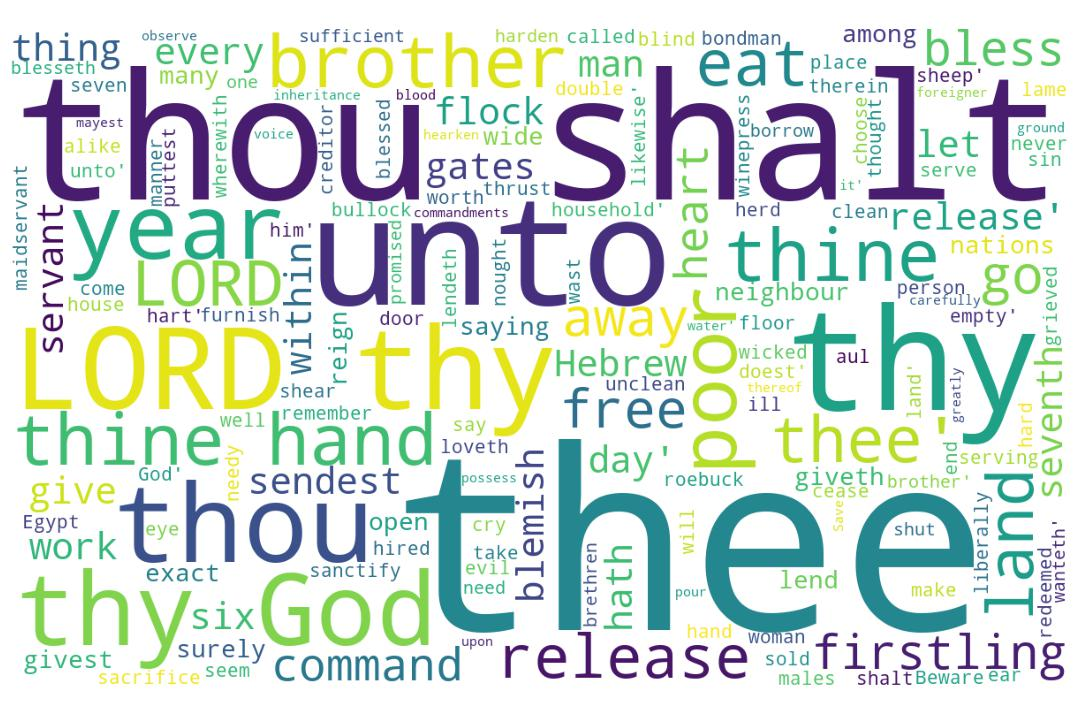
\includegraphics[width=\linewidth]{05OT-Deuteronomy/Deuteronomy15-WordCloud.jpg}
  \caption{Deuteronomy 15 Word Cloud}
  \label{fig:Deuteronomy 15 word Cloud}
\end{figure}

\marginpar{\scriptsize \centering \fcolorbox{bone}{lime}{\textbf{PRINCIPLES OF THE SABBATH}}\\ (Deuteronomy 15:1-23) \begin{compactenum}[I.][8]
    \item  The \textbf{Sabbath}  %\index[scripture]{Deuteronomy!Deu 15:09} \index[scripture]{Deuteronomy!Deu 15:11} (Deuteronomy 19:9, 11)
    \item  \textbf{Sufficiency}  \index[scripture]{Deuteronomy!Deu 15:08} (Deu 15:8)
    \item  The \textbf{Sayings of God}  \index[scripture]{Deuteronomy!Deu 15:09} \index[scripture]{Deuteronomy!Deu 15:11} (Deu 15:9, 11)
    \item  The \textbf{Seventh Year}  \index[scripture]{Deuteronomy!Deu 15:09} \index[scripture]{Deuteronomy!Deu 15:12} (Deu 15:9, 12)
    \item  The \textbf{Sending}  \index[scripture]{Deuteronomy!Deu 15:13}  (Deu 15:13)
    \item  The \textbf{Servants}  \index[scripture]{Deuteronomy!Deu 15:17} \index[scripture]{Deuteronomy!Deu 15:17} (Deu 15:17, 18)
    \item  \textbf{Society}  %\index[scripture]{Deuteronomy!Deu 15:09} \index[scripture]{Deuteronomy!Deu 15:11} (Deuteronomy 19:9, 11)
    \item  Something to \textbf{Sanctify}  \index[scripture]{Deuteronomy!Deu 15:19} (Deu 15:19)
\end{compactenum}}



\footnote{\textcolor[cmyk]{0.99998,1,0,0}{\hyperlink{TOC}{Return to end of Table of Contents.}}}\footnote{\href{https://audiobible.com/bible/deuteronomy_15.html}{\textcolor[cmyk]{0.99998,1,0,0}{Deuteronomy 15 Audio}}}\textcolor[cmyk]{0.99998,1,0,0}{At the end of \emph{every} seven years thou shalt make a release.}
[2] \textcolor[cmyk]{0.99998,1,0,0}{And this \emph{is} the manner of the release: Every creditor that lendeth \emph{ought} unto his neighbour shall release \emph{it}; he shall not exact \emph{it} of his neighbour, or of his brother; because it is called the LORD'S release.}
[3] \textcolor[cmyk]{0.99998,1,0,0}{Of a foreigner thou mayest exact \emph{it} \emph{again}: but \emph{that} which is thine with thy brother thine hand shall release;}
[4] \textcolor[cmyk]{0.99998,1,0,0}{Save when there shall be no poor among you; for the LORD shall greatly bless thee in the land which the LORD thy God giveth thee \emph{for} an inheritance to possess it:}
[5] \textcolor[cmyk]{0.99998,1,0,0}{Only if thou carefully hearken unto the voice of the LORD thy God, to observe to do all these commandments which I command thee this day.}
[6] \textcolor[cmyk]{0.99998,1,0,0}{For the LORD thy God blesseth thee, as he promised thee: and thou shalt lend unto many nations, but thou shalt not borrow; and thou shalt reign over many nations, but they shall not reign over thee.}\\
\\
\P \textcolor[cmyk]{0.99998,1,0,0}{If there be among you a poor man of one of thy brethren within any of thy gates in thy land which the LORD thy God giveth thee, thou shalt not harden thine heart, nor shut thine hand from thy poor brother:}
[8] \textcolor[cmyk]{0.99998,1,0,0}{But thou shalt open thine hand wide unto him, and shalt surely lend him \fcolorbox{bone}{lime}{sufficient} for his need, \emph{in} \emph{that} which he wanteth.}
[9] \textcolor[cmyk]{0.99998,1,0,0}{Beware that there be not a thought in thy wicked heart, \fcolorbox{bone}{lime}{saying}, The \fcolorbox{bone}{lime}{seventh} year, the year of release, is at hand; and thine eye be evil against thy poor brother, and thou givest him nought; and he cry unto the LORD against thee, and it be sin unto thee.}
[10] \textcolor[cmyk]{0.99998,1,0,0}{Thou shalt surely give him, and thine heart shall not be grieved when thou givest unto him: because that for this thing the LORD thy God shall bless thee in all thy works, and in all that thou puttest thine hand unto.}
[11] \textcolor[cmyk]{0.99998,1,0,0}{For the poor shall never cease out of the land: therefore I command thee, \fcolorbox{bone}{lime}{saying}, Thou shalt open thine hand wide unto thy brother, to thy poor, and to thy needy, in thy land.}\\
\\
\P \textcolor[cmyk]{0.99998,1,0,0}{\emph{And} if thy brother, an Hebrew man, or an Hebrew woman, be sold unto thee, and serve thee six years; then in the \fcolorbox{bone}{lime}{seventh} year thou shalt let him go free from thee.}
[13] \textcolor[cmyk]{0.99998,1,0,0}{And when thou sendest him out free from thee, thou shalt not let him go away empty:}
[14] \textcolor[cmyk]{0.99998,1,0,0}{Thou shalt furnish him liberally out of thy flock, and out of thy floor, and out of thy winepress: \emph{of} \emph{that} wherewith the LORD thy God hath blessed thee thou shalt give unto him.}
[15] \textcolor[cmyk]{0.99998,1,0,0}{And thou shalt remember that thou wast a bondman in the land of Egypt, and the LORD thy God redeemed thee: therefore I command thee this thing to day.}
[16] \textcolor[cmyk]{0.99998,1,0,0}{And it shall be, if he say unto thee, I will not go away from thee; because he loveth thee and thine house, because he is well with thee;}
[17] \textcolor[cmyk]{0.99998,1,0,0}{Then thou shalt take an aul, and thrust \emph{it} through his ear unto the door, and he shall be thy \fcolorbox{bone}{lime}{servant} for ever. And also unto thy maidservant thou shalt do likewise.}
[18] \textcolor[cmyk]{0.99998,1,0,0}{It shall not seem hard unto thee, when thou sendest him away free from thee; for he hath been worth a double hired \fcolorbox{bone}{lime}{servant} \emph{to} \emph{thee}, in serving thee six years: and the LORD thy God shall bless thee in all that thou doest.}\\
\\
\P \textcolor[cmyk]{0.99998,1,0,0}{All the firstling males that come of thy herd and of thy flock thou shalt \fcolorbox{bone}{lime}{sanctify} unto the LORD thy God: thou shalt do no work with the firstling of thy bullock, nor shear the firstling of thy sheep.}
[20] \textcolor[cmyk]{0.99998,1,0,0}{Thou shalt eat \emph{it} before the LORD thy God year by year in the place which the LORD shall choose, thou and thy household.}
[21] \textcolor[cmyk]{0.99998,1,0,0}{And if there be \emph{any} blemish therein, \emph{as} \emph{if} \emph{it} \emph{be} lame, or blind, \emph{or} \emph{have} any ill blemish, thou shalt not sacrifice it unto the LORD thy God.}
[22] \textcolor[cmyk]{0.99998,1,0,0}{Thou shalt eat it within thy gates: the unclean and the clean \emph{person} \emph{shall} \emph{eat} \emph{it} alike, as the roebuck, and as the hart.}
[23] \textcolor[cmyk]{0.99998,1,0,0}{Only thou shalt not eat the blood thereof; thou shalt pour it upon the ground as water.}
\index[NWIV]{12!Deuteronomy!Deu 15:1}\index[AWIP]{At!Deuteronomy!Deu 15:1}\index[AWIP]{the!Deuteronomy!Deu 15:1}\index[AWIP]{end!Deuteronomy!Deu 15:1}\index[AWIP]{of!Deuteronomy!Deu 15:1}\index[AWIP]{\emph{every}!Deuteronomy!Deu 15:1}\index[AWIP]{seven!Deuteronomy!Deu 15:1}\index[AWIP]{years!Deuteronomy!Deu 15:1}\index[AWIP]{thou!Deuteronomy!Deu 15:1}\index[AWIP]{shalt!Deuteronomy!Deu 15:1}\index[AWIP]{make!Deuteronomy!Deu 15:1}\index[AWIP]{a!Deuteronomy!Deu 15:1}\index[AWIP]{release!Deuteronomy!Deu 15:1}\index[AWIP]{\emph{every}!Deuteronomy!Deu 15:1}

\index[NWIV]{38!Deuteronomy!Deu 15:2}\index[AWIP]{And!Deuteronomy!Deu 15:2}\index[AWIP]{this!Deuteronomy!Deu 15:2}\index[AWIP]{\emph{is}!Deuteronomy!Deu 15:2}\index[AWIP]{the!Deuteronomy!Deu 15:2}\index[AWIP]{the!Deuteronomy!Deu 15:2 (2)}\index[AWIP]{the!Deuteronomy!Deu 15:2 (3)}\index[AWIP]{manner!Deuteronomy!Deu 15:2}\index[AWIP]{of!Deuteronomy!Deu 15:2}\index[AWIP]{of!Deuteronomy!Deu 15:2 (2)}\index[AWIP]{of!Deuteronomy!Deu 15:2 (3)}\index[AWIP]{release!Deuteronomy!Deu 15:2}\index[AWIP]{release!Deuteronomy!Deu 15:2 (2)}\index[AWIP]{release!Deuteronomy!Deu 15:2 (3)}\index[AWIP]{Every!Deuteronomy!Deu 15:2}\index[AWIP]{creditor!Deuteronomy!Deu 15:2}\index[AWIP]{that!Deuteronomy!Deu 15:2}\index[AWIP]{lendeth!Deuteronomy!Deu 15:2}\index[AWIP]{\emph{ought}!Deuteronomy!Deu 15:2}\index[AWIP]{unto!Deuteronomy!Deu 15:2}\index[AWIP]{his!Deuteronomy!Deu 15:2}\index[AWIP]{his!Deuteronomy!Deu 15:2 (2)}\index[AWIP]{his!Deuteronomy!Deu 15:2 (3)}\index[AWIP]{neighbour!Deuteronomy!Deu 15:2}\index[AWIP]{neighbour!Deuteronomy!Deu 15:2 (2)}\index[AWIP]{shall!Deuteronomy!Deu 15:2}\index[AWIP]{shall!Deuteronomy!Deu 15:2 (2)}\index[AWIP]{\emph{it}!Deuteronomy!Deu 15:2}\index[AWIP]{\emph{it}!Deuteronomy!Deu 15:2 (2)}\index[AWIP]{he!Deuteronomy!Deu 15:2}\index[AWIP]{not!Deuteronomy!Deu 15:2}\index[AWIP]{exact!Deuteronomy!Deu 15:2}\index[AWIP]{or!Deuteronomy!Deu 15:2}\index[AWIP]{brother!Deuteronomy!Deu 15:2}\index[AWIP]{because!Deuteronomy!Deu 15:2}\index[AWIP]{it!Deuteronomy!Deu 15:2}\index[AWIP]{is!Deuteronomy!Deu 15:2}\index[AWIP]{called!Deuteronomy!Deu 15:2}\index[AWIP]{LORD'S!Deuteronomy!Deu 15:2}\index[AWIP]{\emph{is}!Deuteronomy!Deu 15:2}\index[AWIP]{\emph{ought}!Deuteronomy!Deu 15:2}\index[AWIP]{\emph{it}!Deuteronomy!Deu 15:2}\index[AWIP]{\emph{it}!Deuteronomy!Deu 15:2 (2)}

\index[NWIV]{20!Deuteronomy!Deu 15:3}\index[AWIP]{Of!Deuteronomy!Deu 15:3}\index[AWIP]{a!Deuteronomy!Deu 15:3}\index[AWIP]{foreigner!Deuteronomy!Deu 15:3}\index[AWIP]{thou!Deuteronomy!Deu 15:3}\index[AWIP]{mayest!Deuteronomy!Deu 15:3}\index[AWIP]{exact!Deuteronomy!Deu 15:3}\index[AWIP]{\emph{it}!Deuteronomy!Deu 15:3}\index[AWIP]{\emph{again}!Deuteronomy!Deu 15:3}\index[AWIP]{but!Deuteronomy!Deu 15:3}\index[AWIP]{\emph{that}!Deuteronomy!Deu 15:3}\index[AWIP]{which!Deuteronomy!Deu 15:3}\index[AWIP]{is!Deuteronomy!Deu 15:3}\index[AWIP]{thine!Deuteronomy!Deu 15:3}\index[AWIP]{thine!Deuteronomy!Deu 15:3 (2)}\index[AWIP]{with!Deuteronomy!Deu 15:3}\index[AWIP]{thy!Deuteronomy!Deu 15:3}\index[AWIP]{brother!Deuteronomy!Deu 15:3}\index[AWIP]{hand!Deuteronomy!Deu 15:3}\index[AWIP]{shall!Deuteronomy!Deu 15:3}\index[AWIP]{release!Deuteronomy!Deu 15:3}\index[AWIP]{\emph{it}!Deuteronomy!Deu 15:3}\index[AWIP]{\emph{again}!Deuteronomy!Deu 15:3}\index[AWIP]{\emph{that}!Deuteronomy!Deu 15:3}

\index[NWIV]{32!Deuteronomy!Deu 15:4}\index[AWIP]{Save!Deuteronomy!Deu 15:4}\index[AWIP]{when!Deuteronomy!Deu 15:4}\index[AWIP]{there!Deuteronomy!Deu 15:4}\index[AWIP]{shall!Deuteronomy!Deu 15:4}\index[AWIP]{shall!Deuteronomy!Deu 15:4 (2)}\index[AWIP]{be!Deuteronomy!Deu 15:4}\index[AWIP]{no!Deuteronomy!Deu 15:4}\index[AWIP]{poor!Deuteronomy!Deu 15:4}\index[AWIP]{among!Deuteronomy!Deu 15:4}\index[AWIP]{you!Deuteronomy!Deu 15:4}\index[AWIP]{for!Deuteronomy!Deu 15:4}\index[AWIP]{the!Deuteronomy!Deu 15:4}\index[AWIP]{the!Deuteronomy!Deu 15:4 (2)}\index[AWIP]{the!Deuteronomy!Deu 15:4 (3)}\index[AWIP]{LORD!Deuteronomy!Deu 15:4}\index[AWIP]{LORD!Deuteronomy!Deu 15:4 (2)}\index[AWIP]{greatly!Deuteronomy!Deu 15:4}\index[AWIP]{bless!Deuteronomy!Deu 15:4}\index[AWIP]{thee!Deuteronomy!Deu 15:4}\index[AWIP]{thee!Deuteronomy!Deu 15:4 (2)}\index[AWIP]{in!Deuteronomy!Deu 15:4}\index[AWIP]{land!Deuteronomy!Deu 15:4}\index[AWIP]{which!Deuteronomy!Deu 15:4}\index[AWIP]{thy!Deuteronomy!Deu 15:4}\index[AWIP]{God!Deuteronomy!Deu 15:4}\index[AWIP]{giveth!Deuteronomy!Deu 15:4}\index[AWIP]{\emph{for}!Deuteronomy!Deu 15:4}\index[AWIP]{an!Deuteronomy!Deu 15:4}\index[AWIP]{inheritance!Deuteronomy!Deu 15:4}\index[AWIP]{to!Deuteronomy!Deu 15:4}\index[AWIP]{possess!Deuteronomy!Deu 15:4}\index[AWIP]{it!Deuteronomy!Deu 15:4}\index[AWIP]{\emph{for}!Deuteronomy!Deu 15:4}

\index[NWIV]{26!Deuteronomy!Deu 15:5}\index[AWIP]{Only!Deuteronomy!Deu 15:5}\index[AWIP]{if!Deuteronomy!Deu 15:5}\index[AWIP]{thou!Deuteronomy!Deu 15:5}\index[AWIP]{carefully!Deuteronomy!Deu 15:5}\index[AWIP]{hearken!Deuteronomy!Deu 15:5}\index[AWIP]{unto!Deuteronomy!Deu 15:5}\index[AWIP]{the!Deuteronomy!Deu 15:5}\index[AWIP]{the!Deuteronomy!Deu 15:5 (2)}\index[AWIP]{voice!Deuteronomy!Deu 15:5}\index[AWIP]{of!Deuteronomy!Deu 15:5}\index[AWIP]{LORD!Deuteronomy!Deu 15:5}\index[AWIP]{thy!Deuteronomy!Deu 15:5}\index[AWIP]{God!Deuteronomy!Deu 15:5}\index[AWIP]{to!Deuteronomy!Deu 15:5}\index[AWIP]{to!Deuteronomy!Deu 15:5 (2)}\index[AWIP]{observe!Deuteronomy!Deu 15:5}\index[AWIP]{do!Deuteronomy!Deu 15:5}\index[AWIP]{all!Deuteronomy!Deu 15:5}\index[AWIP]{these!Deuteronomy!Deu 15:5}\index[AWIP]{commandments!Deuteronomy!Deu 15:5}\index[AWIP]{which!Deuteronomy!Deu 15:5}\index[AWIP]{I!Deuteronomy!Deu 15:5}\index[AWIP]{command!Deuteronomy!Deu 15:5}\index[AWIP]{thee!Deuteronomy!Deu 15:5}\index[AWIP]{this!Deuteronomy!Deu 15:5}\index[AWIP]{day!Deuteronomy!Deu 15:5}

\index[NWIV]{37!Deuteronomy!Deu 15:6}\index[AWIP]{For!Deuteronomy!Deu 15:6}\index[AWIP]{the!Deuteronomy!Deu 15:6}\index[AWIP]{LORD!Deuteronomy!Deu 15:6}\index[AWIP]{thy!Deuteronomy!Deu 15:6}\index[AWIP]{God!Deuteronomy!Deu 15:6}\index[AWIP]{blesseth!Deuteronomy!Deu 15:6}\index[AWIP]{thee!Deuteronomy!Deu 15:6}\index[AWIP]{thee!Deuteronomy!Deu 15:6 (2)}\index[AWIP]{thee!Deuteronomy!Deu 15:6 (3)}\index[AWIP]{as!Deuteronomy!Deu 15:6}\index[AWIP]{he!Deuteronomy!Deu 15:6}\index[AWIP]{promised!Deuteronomy!Deu 15:6}\index[AWIP]{and!Deuteronomy!Deu 15:6}\index[AWIP]{and!Deuteronomy!Deu 15:6 (2)}\index[AWIP]{thou!Deuteronomy!Deu 15:6}\index[AWIP]{thou!Deuteronomy!Deu 15:6 (2)}\index[AWIP]{thou!Deuteronomy!Deu 15:6 (3)}\index[AWIP]{shalt!Deuteronomy!Deu 15:6}\index[AWIP]{shalt!Deuteronomy!Deu 15:6 (2)}\index[AWIP]{shalt!Deuteronomy!Deu 15:6 (3)}\index[AWIP]{lend!Deuteronomy!Deu 15:6}\index[AWIP]{unto!Deuteronomy!Deu 15:6}\index[AWIP]{many!Deuteronomy!Deu 15:6}\index[AWIP]{many!Deuteronomy!Deu 15:6 (2)}\index[AWIP]{nations!Deuteronomy!Deu 15:6}\index[AWIP]{nations!Deuteronomy!Deu 15:6 (2)}\index[AWIP]{but!Deuteronomy!Deu 15:6}\index[AWIP]{but!Deuteronomy!Deu 15:6 (2)}\index[AWIP]{not!Deuteronomy!Deu 15:6}\index[AWIP]{not!Deuteronomy!Deu 15:6 (2)}\index[AWIP]{borrow!Deuteronomy!Deu 15:6}\index[AWIP]{reign!Deuteronomy!Deu 15:6}\index[AWIP]{reign!Deuteronomy!Deu 15:6 (2)}\index[AWIP]{over!Deuteronomy!Deu 15:6}\index[AWIP]{over!Deuteronomy!Deu 15:6 (2)}\index[AWIP]{they!Deuteronomy!Deu 15:6}\index[AWIP]{shall!Deuteronomy!Deu 15:6}

\index[NWIV]{42!Deuteronomy!Deu 15:7}\index[AWIP]{If!Deuteronomy!Deu 15:7}\index[AWIP]{there!Deuteronomy!Deu 15:7}\index[AWIP]{be!Deuteronomy!Deu 15:7}\index[AWIP]{among!Deuteronomy!Deu 15:7}\index[AWIP]{you!Deuteronomy!Deu 15:7}\index[AWIP]{a!Deuteronomy!Deu 15:7}\index[AWIP]{poor!Deuteronomy!Deu 15:7}\index[AWIP]{poor!Deuteronomy!Deu 15:7 (2)}\index[AWIP]{man!Deuteronomy!Deu 15:7}\index[AWIP]{of!Deuteronomy!Deu 15:7}\index[AWIP]{of!Deuteronomy!Deu 15:7 (2)}\index[AWIP]{of!Deuteronomy!Deu 15:7 (3)}\index[AWIP]{one!Deuteronomy!Deu 15:7}\index[AWIP]{thy!Deuteronomy!Deu 15:7}\index[AWIP]{thy!Deuteronomy!Deu 15:7 (2)}\index[AWIP]{thy!Deuteronomy!Deu 15:7 (3)}\index[AWIP]{thy!Deuteronomy!Deu 15:7 (4)}\index[AWIP]{thy!Deuteronomy!Deu 15:7 (5)}\index[AWIP]{brethren!Deuteronomy!Deu 15:7}\index[AWIP]{within!Deuteronomy!Deu 15:7}\index[AWIP]{any!Deuteronomy!Deu 15:7}\index[AWIP]{gates!Deuteronomy!Deu 15:7}\index[AWIP]{in!Deuteronomy!Deu 15:7}\index[AWIP]{land!Deuteronomy!Deu 15:7}\index[AWIP]{which!Deuteronomy!Deu 15:7}\index[AWIP]{the!Deuteronomy!Deu 15:7}\index[AWIP]{LORD!Deuteronomy!Deu 15:7}\index[AWIP]{God!Deuteronomy!Deu 15:7}\index[AWIP]{giveth!Deuteronomy!Deu 15:7}\index[AWIP]{thee!Deuteronomy!Deu 15:7}\index[AWIP]{thou!Deuteronomy!Deu 15:7}\index[AWIP]{shalt!Deuteronomy!Deu 15:7}\index[AWIP]{not!Deuteronomy!Deu 15:7}\index[AWIP]{harden!Deuteronomy!Deu 15:7}\index[AWIP]{thine!Deuteronomy!Deu 15:7}\index[AWIP]{thine!Deuteronomy!Deu 15:7 (2)}\index[AWIP]{heart!Deuteronomy!Deu 15:7}\index[AWIP]{nor!Deuteronomy!Deu 15:7}\index[AWIP]{shut!Deuteronomy!Deu 15:7}\index[AWIP]{hand!Deuteronomy!Deu 15:7}\index[AWIP]{from!Deuteronomy!Deu 15:7}\index[AWIP]{brother!Deuteronomy!Deu 15:7}

\index[NWIV]{23!Deuteronomy!Deu 15:8}\index[AWIP]{But!Deuteronomy!Deu 15:8}\index[AWIP]{thou!Deuteronomy!Deu 15:8}\index[AWIP]{shalt!Deuteronomy!Deu 15:8}\index[AWIP]{shalt!Deuteronomy!Deu 15:8 (2)}\index[AWIP]{open!Deuteronomy!Deu 15:8}\index[AWIP]{thine!Deuteronomy!Deu 15:8}\index[AWIP]{hand!Deuteronomy!Deu 15:8}\index[AWIP]{wide!Deuteronomy!Deu 15:8}\index[AWIP]{unto!Deuteronomy!Deu 15:8}\index[AWIP]{him!Deuteronomy!Deu 15:8}\index[AWIP]{him!Deuteronomy!Deu 15:8 (2)}\index[AWIP]{and!Deuteronomy!Deu 15:8}\index[AWIP]{surely!Deuteronomy!Deu 15:8}\index[AWIP]{lend!Deuteronomy!Deu 15:8}\index[AWIP]{sufficient!Deuteronomy!Deu 15:8}\index[AWIP]{for!Deuteronomy!Deu 15:8}\index[AWIP]{his!Deuteronomy!Deu 15:8}\index[AWIP]{need!Deuteronomy!Deu 15:8}\index[AWIP]{\emph{in}!Deuteronomy!Deu 15:8}\index[AWIP]{\emph{that}!Deuteronomy!Deu 15:8}\index[AWIP]{which!Deuteronomy!Deu 15:8}\index[AWIP]{he!Deuteronomy!Deu 15:8}\index[AWIP]{wanteth!Deuteronomy!Deu 15:8}\index[AWIP]{\emph{in}!Deuteronomy!Deu 15:8}\index[AWIP]{\emph{that}!Deuteronomy!Deu 15:8}

\index[NWIV]{50!Deuteronomy!Deu 15:9}\index[AWIP]{Beware!Deuteronomy!Deu 15:9}\index[AWIP]{that!Deuteronomy!Deu 15:9}\index[AWIP]{there!Deuteronomy!Deu 15:9}\index[AWIP]{be!Deuteronomy!Deu 15:9}\index[AWIP]{be!Deuteronomy!Deu 15:9 (2)}\index[AWIP]{be!Deuteronomy!Deu 15:9 (3)}\index[AWIP]{not!Deuteronomy!Deu 15:9}\index[AWIP]{a!Deuteronomy!Deu 15:9}\index[AWIP]{thought!Deuteronomy!Deu 15:9}\index[AWIP]{in!Deuteronomy!Deu 15:9}\index[AWIP]{thy!Deuteronomy!Deu 15:9}\index[AWIP]{thy!Deuteronomy!Deu 15:9 (2)}\index[AWIP]{wicked!Deuteronomy!Deu 15:9}\index[AWIP]{heart!Deuteronomy!Deu 15:9}\index[AWIP]{saying!Deuteronomy!Deu 15:9}\index[AWIP]{The!Deuteronomy!Deu 15:9}\index[AWIP]{seventh!Deuteronomy!Deu 15:9}\index[AWIP]{year!Deuteronomy!Deu 15:9}\index[AWIP]{year!Deuteronomy!Deu 15:9 (2)}\index[AWIP]{the!Deuteronomy!Deu 15:9}\index[AWIP]{the!Deuteronomy!Deu 15:9 (2)}\index[AWIP]{of!Deuteronomy!Deu 15:9}\index[AWIP]{release!Deuteronomy!Deu 15:9}\index[AWIP]{is!Deuteronomy!Deu 15:9}\index[AWIP]{at!Deuteronomy!Deu 15:9}\index[AWIP]{hand!Deuteronomy!Deu 15:9}\index[AWIP]{and!Deuteronomy!Deu 15:9}\index[AWIP]{and!Deuteronomy!Deu 15:9 (2)}\index[AWIP]{and!Deuteronomy!Deu 15:9 (3)}\index[AWIP]{and!Deuteronomy!Deu 15:9 (4)}\index[AWIP]{thine!Deuteronomy!Deu 15:9}\index[AWIP]{eye!Deuteronomy!Deu 15:9}\index[AWIP]{evil!Deuteronomy!Deu 15:9}\index[AWIP]{against!Deuteronomy!Deu 15:9}\index[AWIP]{against!Deuteronomy!Deu 15:9 (2)}\index[AWIP]{poor!Deuteronomy!Deu 15:9}\index[AWIP]{brother!Deuteronomy!Deu 15:9}\index[AWIP]{thou!Deuteronomy!Deu 15:9}\index[AWIP]{givest!Deuteronomy!Deu 15:9}\index[AWIP]{him!Deuteronomy!Deu 15:9}\index[AWIP]{nought!Deuteronomy!Deu 15:9}\index[AWIP]{he!Deuteronomy!Deu 15:9}\index[AWIP]{cry!Deuteronomy!Deu 15:9}\index[AWIP]{unto!Deuteronomy!Deu 15:9}\index[AWIP]{unto!Deuteronomy!Deu 15:9 (2)}\index[AWIP]{LORD!Deuteronomy!Deu 15:9}\index[AWIP]{thee!Deuteronomy!Deu 15:9}\index[AWIP]{thee!Deuteronomy!Deu 15:9 (2)}\index[AWIP]{it!Deuteronomy!Deu 15:9}\index[AWIP]{sin!Deuteronomy!Deu 15:9}

\index[NWIV]{42!Deuteronomy!Deu 15:10}\index[AWIP]{Thou!Deuteronomy!Deu 15:10}\index[AWIP]{shalt!Deuteronomy!Deu 15:10}\index[AWIP]{surely!Deuteronomy!Deu 15:10}\index[AWIP]{give!Deuteronomy!Deu 15:10}\index[AWIP]{him!Deuteronomy!Deu 15:10}\index[AWIP]{him!Deuteronomy!Deu 15:10 (2)}\index[AWIP]{and!Deuteronomy!Deu 15:10}\index[AWIP]{and!Deuteronomy!Deu 15:10 (2)}\index[AWIP]{thine!Deuteronomy!Deu 15:10}\index[AWIP]{thine!Deuteronomy!Deu 15:10 (2)}\index[AWIP]{heart!Deuteronomy!Deu 15:10}\index[AWIP]{shall!Deuteronomy!Deu 15:10}\index[AWIP]{shall!Deuteronomy!Deu 15:10 (2)}\index[AWIP]{not!Deuteronomy!Deu 15:10}\index[AWIP]{be!Deuteronomy!Deu 15:10}\index[AWIP]{grieved!Deuteronomy!Deu 15:10}\index[AWIP]{when!Deuteronomy!Deu 15:10}\index[AWIP]{thou!Deuteronomy!Deu 15:10}\index[AWIP]{thou!Deuteronomy!Deu 15:10 (2)}\index[AWIP]{givest!Deuteronomy!Deu 15:10}\index[AWIP]{unto!Deuteronomy!Deu 15:10}\index[AWIP]{unto!Deuteronomy!Deu 15:10 (2)}\index[AWIP]{because!Deuteronomy!Deu 15:10}\index[AWIP]{that!Deuteronomy!Deu 15:10}\index[AWIP]{that!Deuteronomy!Deu 15:10 (2)}\index[AWIP]{for!Deuteronomy!Deu 15:10}\index[AWIP]{this!Deuteronomy!Deu 15:10}\index[AWIP]{thing!Deuteronomy!Deu 15:10}\index[AWIP]{the!Deuteronomy!Deu 15:10}\index[AWIP]{LORD!Deuteronomy!Deu 15:10}\index[AWIP]{thy!Deuteronomy!Deu 15:10}\index[AWIP]{thy!Deuteronomy!Deu 15:10 (2)}\index[AWIP]{God!Deuteronomy!Deu 15:10}\index[AWIP]{bless!Deuteronomy!Deu 15:10}\index[AWIP]{thee!Deuteronomy!Deu 15:10}\index[AWIP]{in!Deuteronomy!Deu 15:10}\index[AWIP]{in!Deuteronomy!Deu 15:10 (2)}\index[AWIP]{all!Deuteronomy!Deu 15:10}\index[AWIP]{all!Deuteronomy!Deu 15:10 (2)}\index[AWIP]{works!Deuteronomy!Deu 15:10}\index[AWIP]{puttest!Deuteronomy!Deu 15:10}\index[AWIP]{hand!Deuteronomy!Deu 15:10}

\index[NWIV]{34!Deuteronomy!Deu 15:11}\index[AWIP]{For!Deuteronomy!Deu 15:11}\index[AWIP]{the!Deuteronomy!Deu 15:11}\index[AWIP]{the!Deuteronomy!Deu 15:11 (2)}\index[AWIP]{poor!Deuteronomy!Deu 15:11}\index[AWIP]{poor!Deuteronomy!Deu 15:11 (2)}\index[AWIP]{shall!Deuteronomy!Deu 15:11}\index[AWIP]{never!Deuteronomy!Deu 15:11}\index[AWIP]{cease!Deuteronomy!Deu 15:11}\index[AWIP]{out!Deuteronomy!Deu 15:11}\index[AWIP]{of!Deuteronomy!Deu 15:11}\index[AWIP]{land!Deuteronomy!Deu 15:11}\index[AWIP]{land!Deuteronomy!Deu 15:11 (2)}\index[AWIP]{therefore!Deuteronomy!Deu 15:11}\index[AWIP]{I!Deuteronomy!Deu 15:11}\index[AWIP]{command!Deuteronomy!Deu 15:11}\index[AWIP]{thee!Deuteronomy!Deu 15:11}\index[AWIP]{saying!Deuteronomy!Deu 15:11}\index[AWIP]{Thou!Deuteronomy!Deu 15:11}\index[AWIP]{shalt!Deuteronomy!Deu 15:11}\index[AWIP]{open!Deuteronomy!Deu 15:11}\index[AWIP]{thine!Deuteronomy!Deu 15:11}\index[AWIP]{hand!Deuteronomy!Deu 15:11}\index[AWIP]{wide!Deuteronomy!Deu 15:11}\index[AWIP]{unto!Deuteronomy!Deu 15:11}\index[AWIP]{thy!Deuteronomy!Deu 15:11}\index[AWIP]{thy!Deuteronomy!Deu 15:11 (2)}\index[AWIP]{thy!Deuteronomy!Deu 15:11 (3)}\index[AWIP]{thy!Deuteronomy!Deu 15:11 (4)}\index[AWIP]{brother!Deuteronomy!Deu 15:11}\index[AWIP]{to!Deuteronomy!Deu 15:11}\index[AWIP]{to!Deuteronomy!Deu 15:11 (2)}\index[AWIP]{and!Deuteronomy!Deu 15:11}\index[AWIP]{needy!Deuteronomy!Deu 15:11}\index[AWIP]{in!Deuteronomy!Deu 15:11}

\index[NWIV]{33!Deuteronomy!Deu 15:12}\index[AWIP]{\emph{And}!Deuteronomy!Deu 15:12}\index[AWIP]{if!Deuteronomy!Deu 15:12}\index[AWIP]{thy!Deuteronomy!Deu 15:12}\index[AWIP]{brother!Deuteronomy!Deu 15:12}\index[AWIP]{an!Deuteronomy!Deu 15:12}\index[AWIP]{an!Deuteronomy!Deu 15:12 (2)}\index[AWIP]{Hebrew!Deuteronomy!Deu 15:12}\index[AWIP]{Hebrew!Deuteronomy!Deu 15:12 (2)}\index[AWIP]{man!Deuteronomy!Deu 15:12}\index[AWIP]{or!Deuteronomy!Deu 15:12}\index[AWIP]{woman!Deuteronomy!Deu 15:12}\index[AWIP]{be!Deuteronomy!Deu 15:12}\index[AWIP]{sold!Deuteronomy!Deu 15:12}\index[AWIP]{unto!Deuteronomy!Deu 15:12}\index[AWIP]{thee!Deuteronomy!Deu 15:12}\index[AWIP]{thee!Deuteronomy!Deu 15:12 (2)}\index[AWIP]{thee!Deuteronomy!Deu 15:12 (3)}\index[AWIP]{and!Deuteronomy!Deu 15:12}\index[AWIP]{serve!Deuteronomy!Deu 15:12}\index[AWIP]{six!Deuteronomy!Deu 15:12}\index[AWIP]{years!Deuteronomy!Deu 15:12}\index[AWIP]{then!Deuteronomy!Deu 15:12}\index[AWIP]{in!Deuteronomy!Deu 15:12}\index[AWIP]{the!Deuteronomy!Deu 15:12}\index[AWIP]{seventh!Deuteronomy!Deu 15:12}\index[AWIP]{year!Deuteronomy!Deu 15:12}\index[AWIP]{thou!Deuteronomy!Deu 15:12}\index[AWIP]{shalt!Deuteronomy!Deu 15:12}\index[AWIP]{let!Deuteronomy!Deu 15:12}\index[AWIP]{him!Deuteronomy!Deu 15:12}\index[AWIP]{go!Deuteronomy!Deu 15:12}\index[AWIP]{free!Deuteronomy!Deu 15:12}\index[AWIP]{from!Deuteronomy!Deu 15:12}\index[AWIP]{\emph{And}!Deuteronomy!Deu 15:12}

\index[NWIV]{17!Deuteronomy!Deu 15:13}\index[AWIP]{And!Deuteronomy!Deu 15:13}\index[AWIP]{when!Deuteronomy!Deu 15:13}\index[AWIP]{thou!Deuteronomy!Deu 15:13}\index[AWIP]{thou!Deuteronomy!Deu 15:13 (2)}\index[AWIP]{sendest!Deuteronomy!Deu 15:13}\index[AWIP]{him!Deuteronomy!Deu 15:13}\index[AWIP]{him!Deuteronomy!Deu 15:13 (2)}\index[AWIP]{out!Deuteronomy!Deu 15:13}\index[AWIP]{free!Deuteronomy!Deu 15:13}\index[AWIP]{from!Deuteronomy!Deu 15:13}\index[AWIP]{thee!Deuteronomy!Deu 15:13}\index[AWIP]{shalt!Deuteronomy!Deu 15:13}\index[AWIP]{not!Deuteronomy!Deu 15:13}\index[AWIP]{let!Deuteronomy!Deu 15:13}\index[AWIP]{go!Deuteronomy!Deu 15:13}\index[AWIP]{away!Deuteronomy!Deu 15:13}\index[AWIP]{empty!Deuteronomy!Deu 15:13}

\index[NWIV]{34!Deuteronomy!Deu 15:14}\index[AWIP]{Thou!Deuteronomy!Deu 15:14}\index[AWIP]{shalt!Deuteronomy!Deu 15:14}\index[AWIP]{shalt!Deuteronomy!Deu 15:14 (2)}\index[AWIP]{furnish!Deuteronomy!Deu 15:14}\index[AWIP]{him!Deuteronomy!Deu 15:14}\index[AWIP]{him!Deuteronomy!Deu 15:14 (2)}\index[AWIP]{liberally!Deuteronomy!Deu 15:14}\index[AWIP]{out!Deuteronomy!Deu 15:14}\index[AWIP]{out!Deuteronomy!Deu 15:14 (2)}\index[AWIP]{out!Deuteronomy!Deu 15:14 (3)}\index[AWIP]{of!Deuteronomy!Deu 15:14}\index[AWIP]{of!Deuteronomy!Deu 15:14 (2)}\index[AWIP]{of!Deuteronomy!Deu 15:14 (3)}\index[AWIP]{thy!Deuteronomy!Deu 15:14}\index[AWIP]{thy!Deuteronomy!Deu 15:14 (2)}\index[AWIP]{thy!Deuteronomy!Deu 15:14 (3)}\index[AWIP]{thy!Deuteronomy!Deu 15:14 (4)}\index[AWIP]{flock!Deuteronomy!Deu 15:14}\index[AWIP]{and!Deuteronomy!Deu 15:14}\index[AWIP]{and!Deuteronomy!Deu 15:14 (2)}\index[AWIP]{floor!Deuteronomy!Deu 15:14}\index[AWIP]{winepress!Deuteronomy!Deu 15:14}\index[AWIP]{\emph{of}!Deuteronomy!Deu 15:14}\index[AWIP]{\emph{that}!Deuteronomy!Deu 15:14}\index[AWIP]{wherewith!Deuteronomy!Deu 15:14}\index[AWIP]{the!Deuteronomy!Deu 15:14}\index[AWIP]{LORD!Deuteronomy!Deu 15:14}\index[AWIP]{God!Deuteronomy!Deu 15:14}\index[AWIP]{hath!Deuteronomy!Deu 15:14}\index[AWIP]{blessed!Deuteronomy!Deu 15:14}\index[AWIP]{thee!Deuteronomy!Deu 15:14}\index[AWIP]{thou!Deuteronomy!Deu 15:14}\index[AWIP]{give!Deuteronomy!Deu 15:14}\index[AWIP]{unto!Deuteronomy!Deu 15:14}\index[AWIP]{\emph{of}!Deuteronomy!Deu 15:14}\index[AWIP]{\emph{that}!Deuteronomy!Deu 15:14}

\index[NWIV]{29!Deuteronomy!Deu 15:15}\index[AWIP]{And!Deuteronomy!Deu 15:15}\index[AWIP]{thou!Deuteronomy!Deu 15:15}\index[AWIP]{thou!Deuteronomy!Deu 15:15 (2)}\index[AWIP]{shalt!Deuteronomy!Deu 15:15}\index[AWIP]{remember!Deuteronomy!Deu 15:15}\index[AWIP]{that!Deuteronomy!Deu 15:15}\index[AWIP]{wast!Deuteronomy!Deu 15:15}\index[AWIP]{a!Deuteronomy!Deu 15:15}\index[AWIP]{bondman!Deuteronomy!Deu 15:15}\index[AWIP]{in!Deuteronomy!Deu 15:15}\index[AWIP]{the!Deuteronomy!Deu 15:15}\index[AWIP]{the!Deuteronomy!Deu 15:15 (2)}\index[AWIP]{land!Deuteronomy!Deu 15:15}\index[AWIP]{of!Deuteronomy!Deu 15:15}\index[AWIP]{Egypt!Deuteronomy!Deu 15:15}\index[AWIP]{and!Deuteronomy!Deu 15:15}\index[AWIP]{LORD!Deuteronomy!Deu 15:15}\index[AWIP]{thy!Deuteronomy!Deu 15:15}\index[AWIP]{God!Deuteronomy!Deu 15:15}\index[AWIP]{redeemed!Deuteronomy!Deu 15:15}\index[AWIP]{thee!Deuteronomy!Deu 15:15}\index[AWIP]{thee!Deuteronomy!Deu 15:15 (2)}\index[AWIP]{therefore!Deuteronomy!Deu 15:15}\index[AWIP]{I!Deuteronomy!Deu 15:15}\index[AWIP]{command!Deuteronomy!Deu 15:15}\index[AWIP]{this!Deuteronomy!Deu 15:15}\index[AWIP]{thing!Deuteronomy!Deu 15:15}\index[AWIP]{to!Deuteronomy!Deu 15:15}\index[AWIP]{day!Deuteronomy!Deu 15:15}

\index[NWIV]{29!Deuteronomy!Deu 15:16}\index[AWIP]{And!Deuteronomy!Deu 15:16}\index[AWIP]{it!Deuteronomy!Deu 15:16}\index[AWIP]{shall!Deuteronomy!Deu 15:16}\index[AWIP]{be!Deuteronomy!Deu 15:16}\index[AWIP]{if!Deuteronomy!Deu 15:16}\index[AWIP]{he!Deuteronomy!Deu 15:16}\index[AWIP]{he!Deuteronomy!Deu 15:16 (2)}\index[AWIP]{he!Deuteronomy!Deu 15:16 (3)}\index[AWIP]{say!Deuteronomy!Deu 15:16}\index[AWIP]{unto!Deuteronomy!Deu 15:16}\index[AWIP]{thee!Deuteronomy!Deu 15:16}\index[AWIP]{thee!Deuteronomy!Deu 15:16 (2)}\index[AWIP]{thee!Deuteronomy!Deu 15:16 (3)}\index[AWIP]{thee!Deuteronomy!Deu 15:16 (4)}\index[AWIP]{I!Deuteronomy!Deu 15:16}\index[AWIP]{will!Deuteronomy!Deu 15:16}\index[AWIP]{not!Deuteronomy!Deu 15:16}\index[AWIP]{go!Deuteronomy!Deu 15:16}\index[AWIP]{away!Deuteronomy!Deu 15:16}\index[AWIP]{from!Deuteronomy!Deu 15:16}\index[AWIP]{because!Deuteronomy!Deu 15:16}\index[AWIP]{because!Deuteronomy!Deu 15:16 (2)}\index[AWIP]{loveth!Deuteronomy!Deu 15:16}\index[AWIP]{and!Deuteronomy!Deu 15:16}\index[AWIP]{thine!Deuteronomy!Deu 15:16}\index[AWIP]{house!Deuteronomy!Deu 15:16}\index[AWIP]{is!Deuteronomy!Deu 15:16}\index[AWIP]{well!Deuteronomy!Deu 15:16}\index[AWIP]{with!Deuteronomy!Deu 15:16}

\index[NWIV]{32!Deuteronomy!Deu 15:17}\index[AWIP]{Then!Deuteronomy!Deu 15:17}\index[AWIP]{thou!Deuteronomy!Deu 15:17}\index[AWIP]{thou!Deuteronomy!Deu 15:17 (2)}\index[AWIP]{shalt!Deuteronomy!Deu 15:17}\index[AWIP]{shalt!Deuteronomy!Deu 15:17 (2)}\index[AWIP]{take!Deuteronomy!Deu 15:17}\index[AWIP]{an!Deuteronomy!Deu 15:17}\index[AWIP]{aul!Deuteronomy!Deu 15:17}\index[AWIP]{and!Deuteronomy!Deu 15:17}\index[AWIP]{and!Deuteronomy!Deu 15:17 (2)}\index[AWIP]{thrust!Deuteronomy!Deu 15:17}\index[AWIP]{\emph{it}!Deuteronomy!Deu 15:17}\index[AWIP]{through!Deuteronomy!Deu 15:17}\index[AWIP]{his!Deuteronomy!Deu 15:17}\index[AWIP]{ear!Deuteronomy!Deu 15:17}\index[AWIP]{unto!Deuteronomy!Deu 15:17}\index[AWIP]{unto!Deuteronomy!Deu 15:17 (2)}\index[AWIP]{the!Deuteronomy!Deu 15:17}\index[AWIP]{door!Deuteronomy!Deu 15:17}\index[AWIP]{he!Deuteronomy!Deu 15:17}\index[AWIP]{shall!Deuteronomy!Deu 15:17}\index[AWIP]{be!Deuteronomy!Deu 15:17}\index[AWIP]{thy!Deuteronomy!Deu 15:17}\index[AWIP]{thy!Deuteronomy!Deu 15:17 (2)}\index[AWIP]{servant!Deuteronomy!Deu 15:17}\index[AWIP]{for!Deuteronomy!Deu 15:17}\index[AWIP]{ever!Deuteronomy!Deu 15:17}\index[AWIP]{And!Deuteronomy!Deu 15:17}\index[AWIP]{also!Deuteronomy!Deu 15:17}\index[AWIP]{maidservant!Deuteronomy!Deu 15:17}\index[AWIP]{do!Deuteronomy!Deu 15:17}\index[AWIP]{likewise!Deuteronomy!Deu 15:17}\index[AWIP]{\emph{it}!Deuteronomy!Deu 15:17}

\index[NWIV]{44!Deuteronomy!Deu 15:18}\index[AWIP]{It!Deuteronomy!Deu 15:18}\index[AWIP]{shall!Deuteronomy!Deu 15:18}\index[AWIP]{shall!Deuteronomy!Deu 15:18 (2)}\index[AWIP]{not!Deuteronomy!Deu 15:18}\index[AWIP]{seem!Deuteronomy!Deu 15:18}\index[AWIP]{hard!Deuteronomy!Deu 15:18}\index[AWIP]{unto!Deuteronomy!Deu 15:18}\index[AWIP]{thee!Deuteronomy!Deu 15:18}\index[AWIP]{thee!Deuteronomy!Deu 15:18 (2)}\index[AWIP]{thee!Deuteronomy!Deu 15:18 (3)}\index[AWIP]{thee!Deuteronomy!Deu 15:18 (4)}\index[AWIP]{when!Deuteronomy!Deu 15:18}\index[AWIP]{thou!Deuteronomy!Deu 15:18}\index[AWIP]{thou!Deuteronomy!Deu 15:18 (2)}\index[AWIP]{sendest!Deuteronomy!Deu 15:18}\index[AWIP]{him!Deuteronomy!Deu 15:18}\index[AWIP]{away!Deuteronomy!Deu 15:18}\index[AWIP]{free!Deuteronomy!Deu 15:18}\index[AWIP]{from!Deuteronomy!Deu 15:18}\index[AWIP]{for!Deuteronomy!Deu 15:18}\index[AWIP]{he!Deuteronomy!Deu 15:18}\index[AWIP]{hath!Deuteronomy!Deu 15:18}\index[AWIP]{been!Deuteronomy!Deu 15:18}\index[AWIP]{worth!Deuteronomy!Deu 15:18}\index[AWIP]{a!Deuteronomy!Deu 15:18}\index[AWIP]{double!Deuteronomy!Deu 15:18}\index[AWIP]{hired!Deuteronomy!Deu 15:18}\index[AWIP]{servant!Deuteronomy!Deu 15:18}\index[AWIP]{\emph{to}!Deuteronomy!Deu 15:18}\index[AWIP]{\emph{thee}!Deuteronomy!Deu 15:18}\index[AWIP]{in!Deuteronomy!Deu 15:18}\index[AWIP]{in!Deuteronomy!Deu 15:18 (2)}\index[AWIP]{serving!Deuteronomy!Deu 15:18}\index[AWIP]{six!Deuteronomy!Deu 15:18}\index[AWIP]{years!Deuteronomy!Deu 15:18}\index[AWIP]{and!Deuteronomy!Deu 15:18}\index[AWIP]{the!Deuteronomy!Deu 15:18}\index[AWIP]{LORD!Deuteronomy!Deu 15:18}\index[AWIP]{thy!Deuteronomy!Deu 15:18}\index[AWIP]{God!Deuteronomy!Deu 15:18}\index[AWIP]{bless!Deuteronomy!Deu 15:18}\index[AWIP]{all!Deuteronomy!Deu 15:18}\index[AWIP]{that!Deuteronomy!Deu 15:18}\index[AWIP]{doest!Deuteronomy!Deu 15:18}\index[AWIP]{\emph{to}!Deuteronomy!Deu 15:18}\index[AWIP]{\emph{thee}!Deuteronomy!Deu 15:18}

\index[NWIV]{39!Deuteronomy!Deu 15:19}\index[AWIP]{All!Deuteronomy!Deu 15:19}\index[AWIP]{the!Deuteronomy!Deu 15:19}\index[AWIP]{the!Deuteronomy!Deu 15:19 (2)}\index[AWIP]{the!Deuteronomy!Deu 15:19 (3)}\index[AWIP]{the!Deuteronomy!Deu 15:19 (4)}\index[AWIP]{firstling!Deuteronomy!Deu 15:19}\index[AWIP]{firstling!Deuteronomy!Deu 15:19 (2)}\index[AWIP]{firstling!Deuteronomy!Deu 15:19 (3)}\index[AWIP]{males!Deuteronomy!Deu 15:19}\index[AWIP]{that!Deuteronomy!Deu 15:19}\index[AWIP]{come!Deuteronomy!Deu 15:19}\index[AWIP]{of!Deuteronomy!Deu 15:19}\index[AWIP]{of!Deuteronomy!Deu 15:19 (2)}\index[AWIP]{of!Deuteronomy!Deu 15:19 (3)}\index[AWIP]{of!Deuteronomy!Deu 15:19 (4)}\index[AWIP]{thy!Deuteronomy!Deu 15:19}\index[AWIP]{thy!Deuteronomy!Deu 15:19 (2)}\index[AWIP]{thy!Deuteronomy!Deu 15:19 (3)}\index[AWIP]{thy!Deuteronomy!Deu 15:19 (4)}\index[AWIP]{thy!Deuteronomy!Deu 15:19 (5)}\index[AWIP]{herd!Deuteronomy!Deu 15:19}\index[AWIP]{and!Deuteronomy!Deu 15:19}\index[AWIP]{flock!Deuteronomy!Deu 15:19}\index[AWIP]{thou!Deuteronomy!Deu 15:19}\index[AWIP]{thou!Deuteronomy!Deu 15:19 (2)}\index[AWIP]{shalt!Deuteronomy!Deu 15:19}\index[AWIP]{shalt!Deuteronomy!Deu 15:19 (2)}\index[AWIP]{sanctify!Deuteronomy!Deu 15:19}\index[AWIP]{unto!Deuteronomy!Deu 15:19}\index[AWIP]{LORD!Deuteronomy!Deu 15:19}\index[AWIP]{God!Deuteronomy!Deu 15:19}\index[AWIP]{do!Deuteronomy!Deu 15:19}\index[AWIP]{no!Deuteronomy!Deu 15:19}\index[AWIP]{work!Deuteronomy!Deu 15:19}\index[AWIP]{with!Deuteronomy!Deu 15:19}\index[AWIP]{bullock!Deuteronomy!Deu 15:19}\index[AWIP]{nor!Deuteronomy!Deu 15:19}\index[AWIP]{shear!Deuteronomy!Deu 15:19}\index[AWIP]{sheep!Deuteronomy!Deu 15:19}

\index[NWIV]{24!Deuteronomy!Deu 15:20}\index[AWIP]{Thou!Deuteronomy!Deu 15:20}\index[AWIP]{shalt!Deuteronomy!Deu 15:20}\index[AWIP]{eat!Deuteronomy!Deu 15:20}\index[AWIP]{\emph{it}!Deuteronomy!Deu 15:20}\index[AWIP]{before!Deuteronomy!Deu 15:20}\index[AWIP]{the!Deuteronomy!Deu 15:20}\index[AWIP]{the!Deuteronomy!Deu 15:20 (2)}\index[AWIP]{the!Deuteronomy!Deu 15:20 (3)}\index[AWIP]{LORD!Deuteronomy!Deu 15:20}\index[AWIP]{LORD!Deuteronomy!Deu 15:20 (2)}\index[AWIP]{thy!Deuteronomy!Deu 15:20}\index[AWIP]{thy!Deuteronomy!Deu 15:20 (2)}\index[AWIP]{God!Deuteronomy!Deu 15:20}\index[AWIP]{year!Deuteronomy!Deu 15:20}\index[AWIP]{year!Deuteronomy!Deu 15:20 (2)}\index[AWIP]{by!Deuteronomy!Deu 15:20}\index[AWIP]{in!Deuteronomy!Deu 15:20}\index[AWIP]{place!Deuteronomy!Deu 15:20}\index[AWIP]{which!Deuteronomy!Deu 15:20}\index[AWIP]{shall!Deuteronomy!Deu 15:20}\index[AWIP]{choose!Deuteronomy!Deu 15:20}\index[AWIP]{thou!Deuteronomy!Deu 15:20}\index[AWIP]{and!Deuteronomy!Deu 15:20}\index[AWIP]{household!Deuteronomy!Deu 15:20}\index[AWIP]{\emph{it}!Deuteronomy!Deu 15:20}

\index[NWIV]{29!Deuteronomy!Deu 15:21}\index[AWIP]{And!Deuteronomy!Deu 15:21}\index[AWIP]{if!Deuteronomy!Deu 15:21}\index[AWIP]{there!Deuteronomy!Deu 15:21}\index[AWIP]{be!Deuteronomy!Deu 15:21}\index[AWIP]{\emph{any}!Deuteronomy!Deu 15:21}\index[AWIP]{blemish!Deuteronomy!Deu 15:21}\index[AWIP]{blemish!Deuteronomy!Deu 15:21 (2)}\index[AWIP]{therein!Deuteronomy!Deu 15:21}\index[AWIP]{\emph{as}!Deuteronomy!Deu 15:21}\index[AWIP]{\emph{if}!Deuteronomy!Deu 15:21}\index[AWIP]{\emph{it}!Deuteronomy!Deu 15:21}\index[AWIP]{\emph{be}!Deuteronomy!Deu 15:21}\index[AWIP]{lame!Deuteronomy!Deu 15:21}\index[AWIP]{or!Deuteronomy!Deu 15:21}\index[AWIP]{blind!Deuteronomy!Deu 15:21}\index[AWIP]{\emph{or}!Deuteronomy!Deu 15:21}\index[AWIP]{\emph{have}!Deuteronomy!Deu 15:21}\index[AWIP]{any!Deuteronomy!Deu 15:21}\index[AWIP]{ill!Deuteronomy!Deu 15:21}\index[AWIP]{thou!Deuteronomy!Deu 15:21}\index[AWIP]{shalt!Deuteronomy!Deu 15:21}\index[AWIP]{not!Deuteronomy!Deu 15:21}\index[AWIP]{sacrifice!Deuteronomy!Deu 15:21}\index[AWIP]{it!Deuteronomy!Deu 15:21}\index[AWIP]{unto!Deuteronomy!Deu 15:21}\index[AWIP]{the!Deuteronomy!Deu 15:21}\index[AWIP]{LORD!Deuteronomy!Deu 15:21}\index[AWIP]{thy!Deuteronomy!Deu 15:21}\index[AWIP]{God!Deuteronomy!Deu 15:21}\index[AWIP]{\emph{any}!Deuteronomy!Deu 15:21}\index[AWIP]{\emph{as}!Deuteronomy!Deu 15:21}\index[AWIP]{\emph{if}!Deuteronomy!Deu 15:21}\index[AWIP]{\emph{it}!Deuteronomy!Deu 15:21}\index[AWIP]{\emph{be}!Deuteronomy!Deu 15:21}\index[AWIP]{\emph{or}!Deuteronomy!Deu 15:21}\index[AWIP]{\emph{have}!Deuteronomy!Deu 15:21}

\index[NWIV]{24!Deuteronomy!Deu 15:22}\index[AWIP]{Thou!Deuteronomy!Deu 15:22}\index[AWIP]{shalt!Deuteronomy!Deu 15:22}\index[AWIP]{eat!Deuteronomy!Deu 15:22}\index[AWIP]{it!Deuteronomy!Deu 15:22}\index[AWIP]{within!Deuteronomy!Deu 15:22}\index[AWIP]{thy!Deuteronomy!Deu 15:22}\index[AWIP]{gates!Deuteronomy!Deu 15:22}\index[AWIP]{the!Deuteronomy!Deu 15:22}\index[AWIP]{the!Deuteronomy!Deu 15:22 (2)}\index[AWIP]{the!Deuteronomy!Deu 15:22 (3)}\index[AWIP]{the!Deuteronomy!Deu 15:22 (4)}\index[AWIP]{unclean!Deuteronomy!Deu 15:22}\index[AWIP]{and!Deuteronomy!Deu 15:22}\index[AWIP]{and!Deuteronomy!Deu 15:22 (2)}\index[AWIP]{clean!Deuteronomy!Deu 15:22}\index[AWIP]{\emph{person}!Deuteronomy!Deu 15:22}\index[AWIP]{\emph{shall}!Deuteronomy!Deu 15:22}\index[AWIP]{\emph{eat}!Deuteronomy!Deu 15:22}\index[AWIP]{\emph{it}!Deuteronomy!Deu 15:22}\index[AWIP]{alike!Deuteronomy!Deu 15:22}\index[AWIP]{as!Deuteronomy!Deu 15:22}\index[AWIP]{as!Deuteronomy!Deu 15:22 (2)}\index[AWIP]{roebuck!Deuteronomy!Deu 15:22}\index[AWIP]{hart!Deuteronomy!Deu 15:22}\index[AWIP]{\emph{person}!Deuteronomy!Deu 15:22}\index[AWIP]{\emph{shall}!Deuteronomy!Deu 15:22}\index[AWIP]{\emph{eat}!Deuteronomy!Deu 15:22}\index[AWIP]{\emph{it}!Deuteronomy!Deu 15:22}

\index[NWIV]{17!Deuteronomy!Deu 15:23}\index[AWIP]{Only!Deuteronomy!Deu 15:23}\index[AWIP]{thou!Deuteronomy!Deu 15:23}\index[AWIP]{thou!Deuteronomy!Deu 15:23 (2)}\index[AWIP]{shalt!Deuteronomy!Deu 15:23}\index[AWIP]{shalt!Deuteronomy!Deu 15:23 (2)}\index[AWIP]{not!Deuteronomy!Deu 15:23}\index[AWIP]{eat!Deuteronomy!Deu 15:23}\index[AWIP]{the!Deuteronomy!Deu 15:23}\index[AWIP]{the!Deuteronomy!Deu 15:23 (2)}\index[AWIP]{blood!Deuteronomy!Deu 15:23}\index[AWIP]{thereof!Deuteronomy!Deu 15:23}\index[AWIP]{pour!Deuteronomy!Deu 15:23}\index[AWIP]{it!Deuteronomy!Deu 15:23}\index[AWIP]{upon!Deuteronomy!Deu 15:23}\index[AWIP]{ground!Deuteronomy!Deu 15:23}\index[AWIP]{as!Deuteronomy!Deu 15:23}\index[AWIP]{water!Deuteronomy!Deu 15:23}


\section{Deuteronomy 15 Outlines}

\subsection{My Outlines}

\subsubsection{Principles of the Sabbath}
\index[speaker]{Keith Anthony!Deuteronomy 15 (Principles of the Sabbath)}
\index[series]{Deuteronomy (Keith Anthony)!Deuteronomy 15 (Principles of the Sabbath)}
\index[date]{2018/02/25!Deuteronomy 15 (Principles of the Sabbath) (Keith Anthony)}

\begin{compactenum}[I.] 
    \item  The \textbf{Sabbath}  %\index[scripture]{Deuteronomy!Deu 15:09} \index[scripture]{Deuteronomy!Deu 15:11} (Deuteronomy 19:9, 11)
    \item  \textbf{Sufficiency}  \index[scripture]{Deuteronomy!Deu 15:08} (Deu 15:8)
    \item  The \textbf{Sayings of God}  \index[scripture]{Deuteronomy!Deu 15:09} \index[scripture]{Deuteronomy!Deu 15:11} (Deu 15:9, 11)
    \item  The \textbf{Seventh Year}  \index[scripture]{Deuteronomy!Deu 15:09} \index[scripture]{Deuteronomy!Deu 15:12} (Deu 15:9, 12)
    \item  The \textbf{Sending}  \index[scripture]{Deuteronomy!Deu 15:13}  (Deu 15:13)
    \item  The \textbf{Servants}  \index[scripture]{Deuteronomy!Deu 15:17} \index[scripture]{Deuteronomy!Deu 15:17} (Deu 15:17, 18)
    \item  \textbf{Society}  %\index[scripture]{Deuteronomy!Deu 15:09} \index[scripture]{Deuteronomy!Deu 15:11} (Deuteronomy 19:9, 11)
    \item  Something to \textbf{Sanctify}  \index[scripture]{Deuteronomy!Deu 15:19} (Deu 15:19)
\end{compactenum}
\subsection{My Outlines from Others}


\section{Deuteronomy 15 Comments}



\chapter{Psalm 57}



\marginpar{\scriptsize \centering \fcolorbox{bone}{lime}{\textbf{GOD"S EVERYDAY ATTRIBUTES}}\\ (Psalm 57:1-22) \begin{compactenum}[I.][8]
    \item \textbf{Abundantness} 
    \item \textbf{Aboveness} 
    \item \textbf{Alongsideness} \index[scripture]{SoS!SoS 04:08}\index[scripture]{Psalms!Psa 057:11} (Psa 57:11) 
    \item \textbf{Aforeness} 
    \item \textbf{Aroundness} 
    \item \textbf{Absoluteness} 
    \item \textbf{Amongness} \index[scripture]{Matthew!Matt 18:20}(Matt 18:20) 
    \item \textbf{Awareness} 
    \item \textbf{Alwaysness} 
    \item \textbf{Attentivness}
    \item \textbf{Availability} \index[scripture]{Jeremiah!Jer 33:03} (Jer 33:3)
\end{compactenum}}



\footnote{\textcolor[cmyk]{0.99998,1,0,0}{\hyperlink{TOC}{Return to end of Table of Contents.}}}\footnote{\href{https://audiobible.com/bible/psalms_57.html}{\textcolor[cmyk]{0.99998,1,0,0}{Psalm 57 Audio}}}\textcolor[cmyk]{0.99998,1,0,0}{To the chief Musician, Al-taschith, Michtam of David, when he fled from Saul in the cave.}\\
\\
\textcolor[cmyk]{0.99998,1,0,0}{Be merciful unto me, O God, be merciful unto me: for my soul trusteth in thee: yea, in the shadow of thy wings will I make my refuge, until \emph{these} calamities be overpast.}
[2] \textcolor[cmyk]{0.99998,1,0,0}{I will cry unto God most high; unto God that performeth \emph{all} \emph{things} for me.}
[3] \textcolor[cmyk]{0.99998,1,0,0}{He shall send from heaven, and save me \emph{from} the reproach of him that would swallow me up. Selah. God shall send forth his mercy and his truth.}\footnote{\textbf{Psalm 50:4-5} - He shall call to the heavens from above, and to the earth, that he may judge his people. 5 Gather my saints together unto me; those that have made a covenant with me by sacrifice.}\footnote{\textbf{Isaiah 26:20} - Come, my people, enter thou into thy chambers, and shut thy doors about thee: hide thyself as it were for a little moment, until the indignation be overpast.}\footnote{\textbf{Hebres 9:28} - So Christ was once offered to bear the sins of many; and unto them that look for him shall he appear the second time without sin unto salvation.}
[4] \textcolor[cmyk]{0.99998,1,0,0}{My soul \emph{is} among lions: \emph{and} I lie \emph{even} \emph{among} them that are set on fire, \emph{even} the sons of men, whose teeth \emph{are} spears and arrows, and their tongue a sharp sword.}\footnote{\textbf{1 Peter 5:8} -  Be sober, be vigilant; because your adversary the devil, as a roaring lion, walketh about, seeking whom he may devour:}
[5] \textcolor[cmyk]{0.99998,1,0,0}{Be thou exalted, O God, above the heavens; \emph{let} thy glory \emph{be} above all the earth.}
[6] \textcolor[cmyk]{0.99998,1,0,0}{They have prepared a net for my steps; my soul is bowed down: they have digged a pit before me, into the midst whereof they are fallen \emph{themselves}. Selah.}
[7] \textcolor[cmyk]{0.99998,1,0,0}{My heart is fixed, O God, my heart is fixed: I will sing and give praise.}
[8] \textcolor[cmyk]{0.99998,1,0,0}{Awake up, my glory; awake, psaltery and harp: I \emph{myself} will awake early.}
[9] \textcolor[cmyk]{0.99998,1,0,0}{I will praise thee, O Lord, among the people: I will sing unto thee among the nations.}
[10] \textcolor[cmyk]{0.99998,1,0,0}{For thy mercy \emph{is} great unto the heavens, and thy truth unto the clouds.}
[11] \textcolor[cmyk]{0.99998,1,0,0}{Be thou exalted, O God, above the heavens: \emph{let} thy glory \emph{be} above all the earth.}



\index[NWIV]{33!Psalms!Psa 57:11}\index[AWIP]{Be!Psalms!Psa 57:11}\index[AWIP]{merciful!Psalms!Psa 57:11}\index[AWIP]{merciful!Psalms!Psa 57:11 (2)}\index[AWIP]{unto!Psalms!Psa 57:11}\index[AWIP]{unto!Psalms!Psa 57:11 (2)}\index[AWIP]{me!Psalms!Psa 57:11}\index[AWIP]{me!Psalms!Psa 57:11 (2)}\index[AWIP]{O!Psalms!Psa 57:11}\index[AWIP]{God!Psalms!Psa 57:11}\index[AWIP]{be!Psalms!Psa 57:11}\index[AWIP]{be!Psalms!Psa 57:11 (2)}\index[AWIP]{for!Psalms!Psa 57:11}\index[AWIP]{my!Psalms!Psa 57:11}\index[AWIP]{my!Psalms!Psa 57:11 (2)}\index[AWIP]{soul!Psalms!Psa 57:11}\index[AWIP]{trusteth!Psalms!Psa 57:11}\index[AWIP]{in!Psalms!Psa 57:11}\index[AWIP]{in!Psalms!Psa 57:11 (2)}\index[AWIP]{thee!Psalms!Psa 57:11}\index[AWIP]{yea!Psalms!Psa 57:11}\index[AWIP]{the!Psalms!Psa 57:11}\index[AWIP]{shadow!Psalms!Psa 57:11}\index[AWIP]{of!Psalms!Psa 57:11}\index[AWIP]{thy!Psalms!Psa 57:11}\index[AWIP]{wings!Psalms!Psa 57:11}\index[AWIP]{will!Psalms!Psa 57:11}\index[AWIP]{I!Psalms!Psa 57:11}\index[AWIP]{make!Psalms!Psa 57:11}\index[AWIP]{refuge!Psalms!Psa 57:11}\index[AWIP]{until!Psalms!Psa 57:11}\index[AWIP]{\emph{these}!Psalms!Psa 57:11}\index[AWIP]{calamities!Psalms!Psa 57:11}\index[AWIP]{overpast!Psalms!Psa 57:11}\index[AWIP]{\emph{these}!Psalms!Psa 57:11}

\index[NWIV]{15!Psalms!Psa 57:2}\index[AWIP]{I!Psalms!Psa 57:2}\index[AWIP]{will!Psalms!Psa 57:2}\index[AWIP]{cry!Psalms!Psa 57:2}\index[AWIP]{unto!Psalms!Psa 57:2}\index[AWIP]{unto!Psalms!Psa 57:2 (2)}\index[AWIP]{God!Psalms!Psa 57:2}\index[AWIP]{God!Psalms!Psa 57:2 (2)}\index[AWIP]{most!Psalms!Psa 57:2}\index[AWIP]{high!Psalms!Psa 57:2}\index[AWIP]{that!Psalms!Psa 57:2}\index[AWIP]{performeth!Psalms!Psa 57:2}\index[AWIP]{\emph{all}!Psalms!Psa 57:2}\index[AWIP]{\emph{things}!Psalms!Psa 57:2}\index[AWIP]{for!Psalms!Psa 57:2}\index[AWIP]{me!Psalms!Psa 57:2}\index[AWIP]{\emph{all}!Psalms!Psa 57:2}\index[AWIP]{\emph{things}!Psalms!Psa 57:2}

\index[NWIV]{28!Psalms!Psa 57:3}\index[AWIP]{He!Psalms!Psa 57:3}\index[AWIP]{shall!Psalms!Psa 57:3}\index[AWIP]{shall!Psalms!Psa 57:3 (2)}\index[AWIP]{send!Psalms!Psa 57:3}\index[AWIP]{send!Psalms!Psa 57:3 (2)}\index[AWIP]{from!Psalms!Psa 57:3}\index[AWIP]{heaven!Psalms!Psa 57:3}\index[AWIP]{and!Psalms!Psa 57:3}\index[AWIP]{and!Psalms!Psa 57:3 (2)}\index[AWIP]{save!Psalms!Psa 57:3}\index[AWIP]{me!Psalms!Psa 57:3}\index[AWIP]{me!Psalms!Psa 57:3 (2)}\index[AWIP]{\emph{from}!Psalms!Psa 57:3}\index[AWIP]{the!Psalms!Psa 57:3}\index[AWIP]{reproach!Psalms!Psa 57:3}\index[AWIP]{of!Psalms!Psa 57:3}\index[AWIP]{him!Psalms!Psa 57:3}\index[AWIP]{that!Psalms!Psa 57:3}\index[AWIP]{would!Psalms!Psa 57:3}\index[AWIP]{swallow!Psalms!Psa 57:3}\index[AWIP]{up!Psalms!Psa 57:3}\index[AWIP]{Selah!Psalms!Psa 57:3}\index[AWIP]{God!Psalms!Psa 57:3}\index[AWIP]{forth!Psalms!Psa 57:3}\index[AWIP]{his!Psalms!Psa 57:3}\index[AWIP]{his!Psalms!Psa 57:3 (2)}\index[AWIP]{mercy!Psalms!Psa 57:3}\index[AWIP]{truth!Psalms!Psa 57:3}\index[AWIP]{\emph{from}!Psalms!Psa 57:3}

\index[NWIV]{33!Psalms!Psa 57:4}\index[AWIP]{My!Psalms!Psa 57:4}\index[AWIP]{soul!Psalms!Psa 57:4}\index[AWIP]{\emph{is}!Psalms!Psa 57:4}\index[AWIP]{among!Psalms!Psa 57:4}\index[AWIP]{lions!Psalms!Psa 57:4}\index[AWIP]{\emph{and}!Psalms!Psa 57:4}\index[AWIP]{I!Psalms!Psa 57:4}\index[AWIP]{lie!Psalms!Psa 57:4}\index[AWIP]{\emph{even}!Psalms!Psa 57:4}\index[AWIP]{\emph{even}!Psalms!Psa 57:4 (2)}\index[AWIP]{\emph{among}!Psalms!Psa 57:4}\index[AWIP]{them!Psalms!Psa 57:4}\index[AWIP]{that!Psalms!Psa 57:4}\index[AWIP]{are!Psalms!Psa 57:4}\index[AWIP]{set!Psalms!Psa 57:4}\index[AWIP]{on!Psalms!Psa 57:4}\index[AWIP]{fire!Psalms!Psa 57:4}\index[AWIP]{the!Psalms!Psa 57:4}\index[AWIP]{sons!Psalms!Psa 57:4}\index[AWIP]{of!Psalms!Psa 57:4}\index[AWIP]{men!Psalms!Psa 57:4}\index[AWIP]{whose!Psalms!Psa 57:4}\index[AWIP]{teeth!Psalms!Psa 57:4}\index[AWIP]{\emph{are}!Psalms!Psa 57:4}\index[AWIP]{spears!Psalms!Psa 57:4}\index[AWIP]{and!Psalms!Psa 57:4}\index[AWIP]{and!Psalms!Psa 57:4 (2)}\index[AWIP]{arrows!Psalms!Psa 57:4}\index[AWIP]{their!Psalms!Psa 57:4}\index[AWIP]{tongue!Psalms!Psa 57:4}\index[AWIP]{a!Psalms!Psa 57:4}\index[AWIP]{sharp!Psalms!Psa 57:4}\index[AWIP]{sword!Psalms!Psa 57:4}\index[AWIP]{\emph{is}!Psalms!Psa 57:4}\index[AWIP]{\emph{and}!Psalms!Psa 57:4}\index[AWIP]{\emph{even}!Psalms!Psa 57:4}\index[AWIP]{\emph{even}!Psalms!Psa 57:4 (2)}\index[AWIP]{\emph{among}!Psalms!Psa 57:4}\index[AWIP]{\emph{are}!Psalms!Psa 57:4}

\index[NWIV]{16!Psalms!Psa 57:5}\index[AWIP]{Be!Psalms!Psa 57:5}\index[AWIP]{thou!Psalms!Psa 57:5}\index[AWIP]{exalted!Psalms!Psa 57:5}\index[AWIP]{O!Psalms!Psa 57:5}\index[AWIP]{God!Psalms!Psa 57:5}\index[AWIP]{above!Psalms!Psa 57:5}\index[AWIP]{above!Psalms!Psa 57:5 (2)}\index[AWIP]{the!Psalms!Psa 57:5}\index[AWIP]{the!Psalms!Psa 57:5 (2)}\index[AWIP]{heavens!Psalms!Psa 57:5}\index[AWIP]{\emph{let}!Psalms!Psa 57:5}\index[AWIP]{thy!Psalms!Psa 57:5}\index[AWIP]{glory!Psalms!Psa 57:5}\index[AWIP]{\emph{be}!Psalms!Psa 57:5}\index[AWIP]{all!Psalms!Psa 57:5}\index[AWIP]{earth!Psalms!Psa 57:5}\index[AWIP]{\emph{let}!Psalms!Psa 57:5}\index[AWIP]{\emph{be}!Psalms!Psa 57:5}

\index[NWIV]{29!Psalms!Psa 57:6}\index[AWIP]{They!Psalms!Psa 57:6}\index[AWIP]{have!Psalms!Psa 57:6}\index[AWIP]{have!Psalms!Psa 57:6 (2)}\index[AWIP]{prepared!Psalms!Psa 57:6}\index[AWIP]{a!Psalms!Psa 57:6}\index[AWIP]{a!Psalms!Psa 57:6 (2)}\index[AWIP]{net!Psalms!Psa 57:6}\index[AWIP]{for!Psalms!Psa 57:6}\index[AWIP]{my!Psalms!Psa 57:6}\index[AWIP]{my!Psalms!Psa 57:6 (2)}\index[AWIP]{steps!Psalms!Psa 57:6}\index[AWIP]{soul!Psalms!Psa 57:6}\index[AWIP]{is!Psalms!Psa 57:6}\index[AWIP]{bowed!Psalms!Psa 57:6}\index[AWIP]{down!Psalms!Psa 57:6}\index[AWIP]{they!Psalms!Psa 57:6}\index[AWIP]{they!Psalms!Psa 57:6 (2)}\index[AWIP]{digged!Psalms!Psa 57:6}\index[AWIP]{pit!Psalms!Psa 57:6}\index[AWIP]{before!Psalms!Psa 57:6}\index[AWIP]{me!Psalms!Psa 57:6}\index[AWIP]{into!Psalms!Psa 57:6}\index[AWIP]{the!Psalms!Psa 57:6}\index[AWIP]{midst!Psalms!Psa 57:6}\index[AWIP]{whereof!Psalms!Psa 57:6}\index[AWIP]{are!Psalms!Psa 57:6}\index[AWIP]{fallen!Psalms!Psa 57:6}\index[AWIP]{\emph{themselves}!Psalms!Psa 57:6}\index[AWIP]{Selah!Psalms!Psa 57:6}\index[AWIP]{\emph{themselves}!Psalms!Psa 57:6}

\index[NWIV]{16!Psalms!Psa 57:7}\index[AWIP]{My!Psalms!Psa 57:7}\index[AWIP]{heart!Psalms!Psa 57:7}\index[AWIP]{heart!Psalms!Psa 57:7 (2)}\index[AWIP]{is!Psalms!Psa 57:7}\index[AWIP]{is!Psalms!Psa 57:7 (2)}\index[AWIP]{fixed!Psalms!Psa 57:7}\index[AWIP]{fixed!Psalms!Psa 57:7 (2)}\index[AWIP]{O!Psalms!Psa 57:7}\index[AWIP]{God!Psalms!Psa 57:7}\index[AWIP]{my!Psalms!Psa 57:7}\index[AWIP]{I!Psalms!Psa 57:7}\index[AWIP]{will!Psalms!Psa 57:7}\index[AWIP]{sing!Psalms!Psa 57:7}\index[AWIP]{and!Psalms!Psa 57:7}\index[AWIP]{give!Psalms!Psa 57:7}\index[AWIP]{praise!Psalms!Psa 57:7}

\index[NWIV]{13!Psalms!Psa 57:8}\index[AWIP]{Awake!Psalms!Psa 57:8}\index[AWIP]{up!Psalms!Psa 57:8}\index[AWIP]{my!Psalms!Psa 57:8}\index[AWIP]{glory!Psalms!Psa 57:8}\index[AWIP]{awake!Psalms!Psa 57:8}\index[AWIP]{awake!Psalms!Psa 57:8 (2)}\index[AWIP]{psaltery!Psalms!Psa 57:8}\index[AWIP]{and!Psalms!Psa 57:8}\index[AWIP]{harp!Psalms!Psa 57:8}\index[AWIP]{I!Psalms!Psa 57:8}\index[AWIP]{\emph{myself}!Psalms!Psa 57:8}\index[AWIP]{will!Psalms!Psa 57:8}\index[AWIP]{early!Psalms!Psa 57:8}\index[AWIP]{\emph{myself}!Psalms!Psa 57:8}

\index[NWIV]{17!Psalms!Psa 57:9}\index[AWIP]{I!Psalms!Psa 57:9}\index[AWIP]{I!Psalms!Psa 57:9 (2)}\index[AWIP]{will!Psalms!Psa 57:9}\index[AWIP]{will!Psalms!Psa 57:9 (2)}\index[AWIP]{praise!Psalms!Psa 57:9}\index[AWIP]{thee!Psalms!Psa 57:9}\index[AWIP]{thee!Psalms!Psa 57:9 (2)}\index[AWIP]{O!Psalms!Psa 57:9}\index[AWIP]{Lord!Psalms!Psa 57:9}\index[AWIP]{among!Psalms!Psa 57:9}\index[AWIP]{among!Psalms!Psa 57:9 (2)}\index[AWIP]{the!Psalms!Psa 57:9}\index[AWIP]{the!Psalms!Psa 57:9 (2)}\index[AWIP]{people!Psalms!Psa 57:9}\index[AWIP]{sing!Psalms!Psa 57:9}\index[AWIP]{unto!Psalms!Psa 57:9}\index[AWIP]{nations!Psalms!Psa 57:9}

\index[NWIV]{14!Psalms!Psa 57:10}\index[AWIP]{For!Psalms!Psa 57:10}\index[AWIP]{thy!Psalms!Psa 57:10}\index[AWIP]{thy!Psalms!Psa 57:10 (2)}\index[AWIP]{mercy!Psalms!Psa 57:10}\index[AWIP]{\emph{is}!Psalms!Psa 57:10}\index[AWIP]{great!Psalms!Psa 57:10}\index[AWIP]{unto!Psalms!Psa 57:10}\index[AWIP]{unto!Psalms!Psa 57:10 (2)}\index[AWIP]{the!Psalms!Psa 57:10}\index[AWIP]{the!Psalms!Psa 57:10 (2)}\index[AWIP]{heavens!Psalms!Psa 57:10}\index[AWIP]{and!Psalms!Psa 57:10}\index[AWIP]{truth!Psalms!Psa 57:10}\index[AWIP]{clouds!Psalms!Psa 57:10}\index[AWIP]{\emph{is}!Psalms!Psa 57:10}

\index[NWIV]{16!Psalms!Psa 57:11}\index[AWIP]{Be!Psalms!Psa 57:11}\index[AWIP]{thou!Psalms!Psa 57:11}\index[AWIP]{exalted!Psalms!Psa 57:11}\index[AWIP]{O!Psalms!Psa 57:11}\index[AWIP]{God!Psalms!Psa 57:11}\index[AWIP]{above!Psalms!Psa 57:11}\index[AWIP]{above!Psalms!Psa 57:11 (2)}\index[AWIP]{the!Psalms!Psa 57:11}\index[AWIP]{the!Psalms!Psa 57:11 (2)}\index[AWIP]{heavens!Psalms!Psa 57:11}\index[AWIP]{\emph{let}!Psalms!Psa 57:11}\index[AWIP]{thy!Psalms!Psa 57:11}\index[AWIP]{glory!Psalms!Psa 57:11}\index[AWIP]{\emph{be}!Psalms!Psa 57:11}\index[AWIP]{all!Psalms!Psa 57:11}\index[AWIP]{earth!Psalms!Psa 57:11}\index[AWIP]{\emph{let}!Psalms!Psa 57:11}\index[AWIP]{\emph{be}!Psalms!Psa 57:11}


\section{Psalm 57 Outlines}

\subsection{My Outlines}

\subsubsection{Everyday Attributes of God that I Like}
\textbf{Introduction:} Psalm 57 is one of those Psalms that speak of dark days for David. It speaks of a time when David was in hiding from Saul in a cave, perhaps the cave of Adullam spoken in 1 Samuel 22, or 2 Samuel 23 or 1 Chronicles 11.  Or perhaps a cave in En-gedi spoken of in 1 Samuel 24. In anyc ase, David is running for his life and in hiding from one who wishes to destroy him.  In fact, Psalm 57 pictures the time of Tribulation, and verse 23 even shows a great resuce of the Jews in the middle of the Trobulation. John Phillips speaks of David's \textbf{Calamites} in the psalm, and his \textbf{Crises}, but he also speaks on David's \textbf{Confidence}.(See Phillips) I've had dark times in life, although never to the extent of having to hide from someone who is seeking to kill me, and I'm sure we all have. I am getting older and am starting to experience some health issues -- I definitely do not have the strength and stamina that I used to. I seem to need more naps these days. But one thing that is not failing for me is my relationship with God. And this is mostly because of who God is.  As I spend more time as a Christina, I appreciate God even more, as I learn about who God really is. During my 39 years as a Christian, I come to know some of the ``Everyday attributes of God.'' In Bible school, studying theology, we learned that God is Omnipresent, He is Omniscient, and he is Ominpotent.  He is also holy. But for a few minutes, here, I want to cover some of these everyday attributes. I'll start by saying that this is NOT a complete list. I won't do God justice in my descriptions. And, I haven't worked out the theology for them.
\index[speaker]{Keith Anthony!Psalm 057 (Everyday Attributes of God that I Like)}
\index[series]{Psalms (Keith Anthony)!Psalm 057 (Everyday Attributes of God that I Like)}
\index[date]{2017/02/03!Psalm 057 (Everyday Attributes of God that I Like) (Keith Anthony)}
\begin{compactenum}[I.][19]
    \item \textbf{Abundantness} \index[scripture]{Philippians!Phil 04:19} (Philippians 4:19) But my God shall supply all your need according to his riches in glory by Christ Jesus. God is the pantry that is never empty. He is the well that never runs dry. He is the oil barrel of the widow of Zarepath.
    \item \textbf{Aboveness} I am happy that I have a God who is has aboveness.  He is above the fry. the petty squabbles and even the big ones, do not affect God.  They don't derail his plan. they don't sidetrack his plan. the don't defile his plan.
    \item \textbf{Alongsideness} \index[scripture]{SoS!SoS 04:08}\index[scripture]{Psalms!Psa 057:11} (Psalm 57:11) speaks of, in a romatic sense,the joy of having that special one with you.  ``Come with me from Lebanon, my spouse, with me from Lebanon: look from the top of Amana, from the top of Shenir and Hermon, from the lions’ dens, from the mountains of the leopards. [9] Thou hast ravished my heart, my sister, my spouse; thou hast ravished my heart with one of thine eyes, with one chain of thy neck.'' When everyone you care about is gone, for a Christian God will be right there beside you.
    \item \textbf{Aforeness} During the travels of the Israelites to the Promised Land, they were lead by the Lord%\index[scripture]{Psalms!Psalm 057:05}\index[scripture]{Psalms!Psalm 057:11} (Psalm 57:5, 11)
    \item \textbf{Aroundness} God has ``aroundness''. It is that difficult to see the existence of, evidence of, and presence of God if you are looking.%\index[scripture]{Psalms!Psalm 057:05}\index[scripture]{Psalms!Psalm 057:11} (Psalm 57:5, 11)
    \item \textbf{Absoluteness} %\index[scripture]{Psalms!Psalm 057:05}\index[scripture]{Psalms!Psalm 057:11} (Psalm 57:5, 11)
    \item \textbf{Amongness} \index[scripture]{Matthew!Matt 18:20}(Matt 18:20) Tells us that wherever two or three believers are gathered together is His name, go is among them.   \index[scripture]{Revelation!Rev 01:03} Revelation 1:3 tells is that Jesus is in the midst of the churches.  It is wonderful to kow that the living God, the living Saviour meets with Christians.
    \item \textbf{Awareness} God's omniscience means that he is completely aware of everything about me, everything around me, everything affecting me, everything in store for me, every decision I will have to make (and the results of them)%\index[scripture]{Psalms!Psalm 057:05}\index[scripture]{Psalms!Psalm 057:11} (Psalm 57:5, 11)
    \item \textbf{Alwaysness} This attribute I guess is God's immutability restated. God is completely reliable.God is the guarantee. 100 \% certain. %\index[scripture]{Genesis!Genesis 06:03}\index[scripture]{Exodus!Exodus 27:20}\index[scripture]{2 Thessalonians!2 Thessalonians 3:16} (Genesis 6:3, Exodus 27:20, 2 Thessalonians 3:16)
    \item \textbf{Attentivness} I think of a brand new baby and the attention a mother gives it. Every need is anticipated and met. Everything thing is done with tenderness and 100 per cent focus. God is that way, that he can give every one of his children complete focus, all the time.
    \item \textbf{Availability} \index[scripture]{Jeremiah!Jer 33:03} (Jeremiah 33:3) says ``Call unto me, and I will answer thee, and shew thee great and mighty things, which thou knowest not.''  To the soul who wants God, he is always available. A christian knows that  from scripture. He knows that from experience. He knows that from the testimony of other saints. If you do not HAVE God, He is available right now. 
\end{compactenum}


\subsection{Outlines from Others}


\subsubsection{Hide Me, Oh My Saviour, Hide}
%\textbf{Introduction:} Psalm 57 is one of those Psalms that speak of dark days for David. It speaks of a time when David was in hiding from Saul in a cave, perhaps the cave of Adullam spoken in 1 Samuel 22, or 2 Samuel 23 or 1 Chronicles 11.  Or perhaps a cave in En-gedi spoken of in 1 Samuel 24. In anyc ase, David is running for his life and in hiding from one who wishes to destroy him.  In fact, Psalm 57 pictures the time of Tribulation, and verse 23 even shows a great resuce of the Jews in the middle of the Trobulation. John Phillips speaks of David's \textbf{Calamites} in the psalm, and his \textbf{Crises}, but he also speaks on David's \textbf{Confidence}.\cite{Phillips2001PsalmsV1} I've had dark times in life, although never to the extent of having to hide from someone who is seeking to kill me, and I'm sure we all have. I am getting older and am starting to experience some health issues -- I definitely do not have the strength and stamina that I used to. I seem to need more naps these days. But one thing that is not failing for me is my relationship with God. And this is mostly because of who God is.  As I spend more time as a Christina, I appreciate God even more, as I learn about who God really is. During my 39 years as a Christian, I come to know some of the ``Everyday attributes of God.'' In Bible school, studying theology, we learned that God is Omnipresent, He is Omniscient, and he is Ominpotent.  He is also holy. But for a few minutes, here, I want to cover some of these everyday attributes. I'll start by saying that this is NOT a complete list. I won't do God justice in my descriptions.

\index[speaker]{John Phillips!Psalm 057 (Hide Me, Oh My Saviour, Hide}
\index[speaker]{Psalms (John Phillips)!Psalm 057 (Hide Me, Oh My Saviour, Hide}
\index[date]{2017/02/03!Psalm 057 (Hide Me, Oh My Saviour, Hide\footnote{John Phillips}) (John Phillips)}
\begin{compactenum}[I.][3]
    \item The \textbf{Calamities which Thronged Him} \index[scripture]{Psalms!Psa 057:01--03} (Psalm 57:1--3)\footnote{John Phillips, Exploring the Psalms, Vol I.\cite{Phillips2001ExploringPsalms1}}
	\begin{compactenum}[A.][3]
		\item Lord, Hide Me \index[scripture]{Psalms!Psa 057:01} (Psa 57:1)
		\item Lord, Hear Me \index[scripture]{Psalms!Psa 057:02} (Psa 57:2)
		\item Lord, Help Me \index[scripture]{Psalms!Psa 057:03} (Psa 57:3)
	\end{compactenum}
    \item The \textbf{Crises which Threatened Him} \index[scripture]{Psalms!Psa 057:04--06} (Psa 57:4--6)
	\begin{compactenum}[A.][3]
		\item The Seriousness of his Situation \index[scripture]{Psalms!Psa 057:04} (Psa 57:4)
		\item The Sovereignty of his Saviour \index[scripture]{Psalms!Psa 057:05} (Psa 57:5)
		\item The Significance of his Salvation \index[scripture]{Psalms!Psa 057:06} (Psa 57:6)
	\end{compactenum}
    \item The \textbf{Confidence which Thrillled Him} \index[scripture]{Psalms!Psa 057:07--11} (Psa 57:7--11)
	\begin{compactenum}[A.][3]
		\item A Willing Confidence \index[scripture]{Psalms!Psa 057:07} (Psa 57:7)
		\item A Witnessing Confidence \index[scripture]{Psalms!Psa 057:08--09} (Psa 57:8--9)
		\item A Worshipping Confidence \index[scripture]{Psalms!Psa 057:10--11} (Psa 57:10--11)
	\end{compactenum}
\end{compactenum}
\section{Psalm 57 Comments}

\subsection{Numeric Nuggets}
\textbf{13: } Verse 8 has 13 words. Verses 2 and 7 have 13 unique words.



\chapter{Proverb 26}

\begin{figure}
  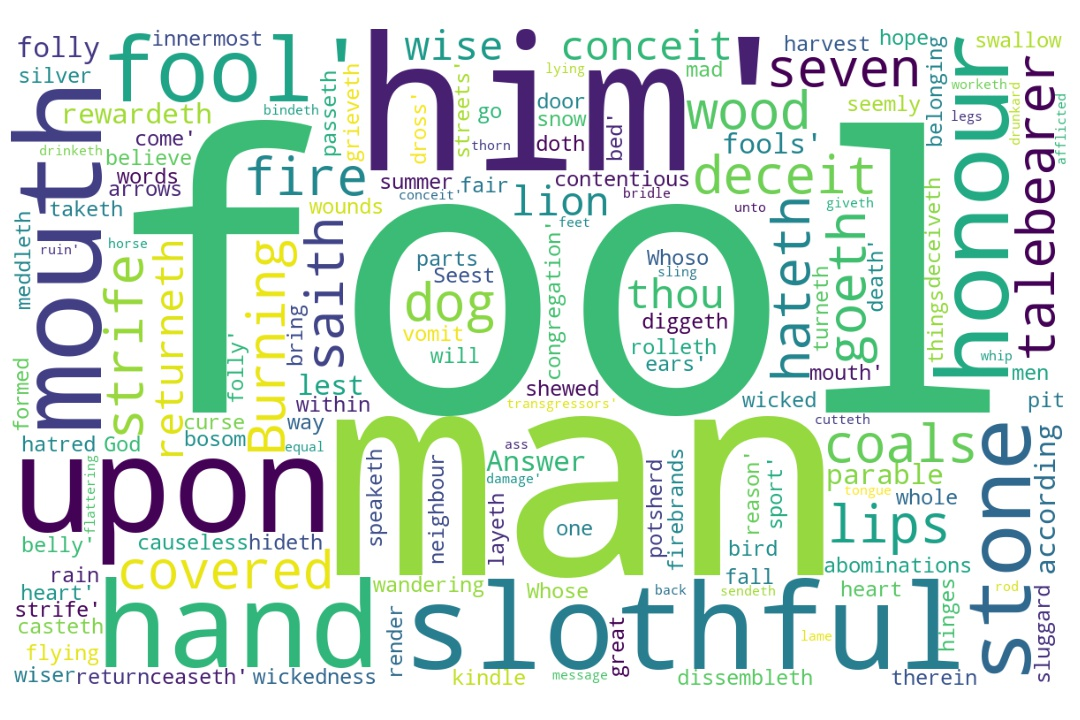
\includegraphics[width=\linewidth]{20OT-Proverbs/Proverb26-WordCloud.jpg}
  \caption{Proverb 26 Word Cloud}
  \label{fig:Proverb 26 word Cloud}
\end{figure}


\marginpar{\scriptsize \centering \fcolorbox{bone}{lime}{\textbf{CHARACTER OF A FOOL}}\\ (Proverb 26:1--28) \begin{compactenum}[I.][8]
    \item \textbf{Uncorrected} \index[scripture]{Proverbs!Pro 26:04}(Pro 26:4) -- one that stays uncorrected, and even worse is proud of that
    \item \textbf{Unreliable} \index[scripture]{Proverbs!Pro 26:06}(Pro 26:6)
    \item \textbf{Unteachable} \index[scripture]{Proverbs!Pro 26:07, 09}(Pro 26:7, 9)
    \item \textbf{Unworthy} \index[scripture]{Proverbs!Pro 26:08}(Pro 26:8) -- of course, we are ultimately all unworthy, but if nothing worthy of praise emerges in a life then perhaps ...
    \item \textbf{Unchangeable} \index[scripture]{Proverbs!Pro 26:11}(Pro 26:11)
    \item \textbf{Unmotivated} \index[scripture]{Proverbs!Pro 26:15}(Pro 26:15)
    \item \textbf{Uncaring} \index[scripture]{Proverbs!Pro 26:28}(Pro 26:28)
\end{compactenum}}

\marginpar{\scriptsize \centering \fcolorbox{bone}{yellow}{\textbf{THE CASTLES OF CONCEIT}}\\ (Proverb 26:1--28)\\The rich, powerful, highly educated: \\
Introduction: see \href{https://www.skywardcoaching.com/single-post/2016/07/13/the-seven-habits-of-highly-uncoachable-people}{The Seven Habits of Highly Un/Coachable People}. Plenty of scriptural examples, such as, Pharaoh, Saul, Nabal, and anyone who rejects the gospel ...
\begin{compactenum}[I.][8]
    \item Think themselves \textbf{Invulnerable and Indestructible} %\index[scripture]{Proverbs!Pro 26:04}(Pro 26:4) -- one that stays uncorrected, and even worse is proud of that
    \item Think themselves \textbf{Impressive}
    \item Think themselves \textbf{Indispensible}
    \item Acts \textbf{Independent} (from God and truth)
    \item Are \textbf{Incorrigible}
    \item Are \textbf{Impetuous} (uncoachable and uncorrectible)
    \item Instead are \textbf{Insecure \& Insubstantial}
\end{compactenum}}

\footnote{\textcolor[cmyk]{0.99998,1,0,0}{\hyperlink{TOC}{Return to end of Table of Contents.}}}\footnote{\href{https://audiobible.com/bible/proverbs_26.html}{\textcolor[cmyk]{0.99998,1,0,0}{Proverbs Audio}}}\textcolor[cmyk]{0.99998,1,0,0}{As snow \fcolorbox{bone}{bone}{in} summer, and as rain \fcolorbox{bone}{bone}{in} harvest, so honour is not seemly for a fool.}
[2] \textcolor[cmyk]{0.99998,1,0,0}{As the bird by wandering, as the swallow by flying, so the curse causeless shall not come.}
[3] \textcolor[cmyk]{0.99998,1,0,0}{A whip for the horse, a bridle for the ass, and a rod for the fool's back.}
[4] \textcolor[cmyk]{0.99998,1,0,0}{Answer not a fool according to his \fcolorbox{bone}{lime}{folly}, lest thou also be like unto him.}
[5] \textcolor[cmyk]{0.99998,1,0,0}{Answer a fool according to his folly, lest he be wise \fcolorbox{bone}{bone}{in} his own conceit.}
[6] \textcolor[cmyk]{0.99998,1,0,0}{He that sendeth a message \fcolorbox{bone}{lime}{by the hand of a fool} cutteth off the feet, \emph{and} drinketh damage.}
[7] \textcolor[cmyk]{0.99998,1,0,0}{The legs of the lame are not equal: so \emph{is} a parable \fcolorbox{bone}{lime}{in the mouth} \fcolorbox{bone}{lime}{of fools}.}
[8] \textcolor[cmyk]{0.99998,1,0,0}{As he that bindeth a stone \fcolorbox{bone}{bone}{in} a sling, so \emph{is} he that giveth \fcolorbox{bone}{lime}{honour to a fool}.}
[9] \textcolor[cmyk]{0.99998,1,0,0}{\emph{As} a thorn goeth up into the hand of a drunkard, so \emph{is} a parable \fcolorbox{bone}{bone}{in} the mouth of fools.}
[10] \textcolor[cmyk]{0.99998,1,0,0}{The great \emph{God} that formed all \emph{things} both rewardeth the fool, and rewardeth \fcolorbox{bone}{MYGOLD}{transgressors}.}
[11] \textcolor[cmyk]{0.99998,1,0,0}{As a dog returneth to his vomit, \emph{so} a fool \fcolorbox{bone}{lime}{returneth} to his folly.}
[12] \textcolor[cmyk]{0.99998,1,0,0}{Seest thou a man wise \fcolorbox{bone}{bone}{in} his own conceit? \emph{there} \emph{is} more hope of a fool than of him.}
[13] \textcolor[cmyk]{0.99998,1,0,0}{The slothful \emph{man} saith, \emph{There} \emph{is} a lion \fcolorbox{bone}{bone}{in} the way; a lion \emph{is} \fcolorbox{bone}{bone}{in} the streets.}
[14] \textcolor[cmyk]{0.99998,1,0,0}{\emph{As} the door turneth upon his hinges, so \emph{doth} the slothful upon his bed.}
[15] \textcolor[cmyk]{0.99998,1,0,0}{The slothful hideth his hand \fcolorbox{bone}{bone}{in} \emph{his} bosom; it \fcolorbox{bone}{lime}{grieveth him} to bring it again to his mouth.}
[16] \textcolor[cmyk]{0.99998,1,0,0}{The sluggard \emph{is} wiser \fcolorbox{bone}{bone}{in} his own conceit than seven men that can render a reason.}
[17] \textcolor[cmyk]{0.99998,1,0,0}{He that passeth by, \emph{and} meddleth with strife \emph{belonging} not to him, \emph{is} \emph{like} one that taketh a dog by the ears.}
[18] \textcolor[cmyk]{0.99998,1,0,0}{As a mad \emph{man} who casteth firebrands, arrows, and death,}
[19] \textcolor[cmyk]{0.99998,1,0,0}{So \emph{is} the man \emph{that} deceiveth his neighbour, and saith, Am not I \fcolorbox{bone}{bone}{in} sport?}
[20] \textcolor[cmyk]{0.99998,1,0,0}{Where no wood is, \emph{there} the fire goeth out: so where \emph{there} \emph{is} no talebearer, the strife ceaseth.}
[21] \textcolor[cmyk]{0.99998,1,0,0}{\emph{As} coals \emph{are} to burning coals, and wood to fire; so \emph{is} a contentious man to kindle strife.}
[22] \textcolor[cmyk]{0.99998,1,0,0}{The words of a talebearer \emph{are} as wounds, and they go down into the innermost parts of the belly.}
[23] \textcolor[cmyk]{0.99998,1,0,0}{Burning lips and a wicked heart \emph{are} \emph{like} a potsherd covered with silver dross.}
[24] \textcolor[cmyk]{0.99998,1,0,0}{He that hateth dissembleth with his lips, and layeth up deceit within him;}
[25] \textcolor[cmyk]{0.99998,1,0,0}{When he speaketh fair, believe him not: for \emph{there} \emph{are} seven abominations \fcolorbox{bone}{bone}{in} his heart.}\footnote{These seven abominations are listen in Proverbs 6:16-19:
\begin{compactenum}
\item A Proud Look
\item A Lying Tongue
\item Hands that Shed Innocent Blood
\item A Heart that Deviseth Wicked Imaginations
\item Feet that a swift to run to mischief
\item A False Witness
\item He that sow discord among brethren
\end{compactenum}
\textbf{Proverbs 6:16-19} - These six things doth the LORD hate: yea, seven are an abomination unto him: [17] A proud look, a lying tongue, and hands that shed innocent blood, [18] An heart that deviseth wicked imaginations, feet that be swift \fcolorbox{bone}{bone}{in} running to mischief, [19] A false witness that speaketh lies, and he that soweth discord among brethren.}
[26] \textcolor[cmyk]{0.99998,1,0,0}{\emph{Whose} hatred is covered by deceit, his wickedness shall be shewed before the \emph{whole} congregation.}
[27] \textcolor[cmyk]{0.99998,1,0,0}{Whoso diggeth a pit shall fall therein: and he that rolleth a stone, it will return upon him.}\footnote{\textbf{Proverb 1:31} -  Therefore shall they eat of the fruit of their own way, and be filled with their own devices.}\footnote{\textbf{Jeremiah 18:12} - And they said, There is no hope: but we will walk after our own devices, and we will every one do the imagination of his evil heart.}
[28] \textcolor[cmyk]{0.99998,1,0,0}{A \fcolorbox{bone}{lime}{lying tongue} hateth \emph{those} \emph{that} \emph{are} afflicted by it; and a flattering mouth worketh ruin.}



\section{Proverb 26 Comments}

\subsection{Numeric Nuggets}
Verse 24 has 13 words.  Verses 10, 23, and 24 have 13 unique words. he word ``in'' is used 13 times n the chapter. The word ``and'' is found 11 times plus 2 times in italics.

\subsection{Proverb 26:4-5}
Do Proverbs 26:4 and 26:5 contradict? How can both verses be true? Proverbs has much to say about fools. They despise wisdom (Proverbs 1:7, 22, 10:21, 23:9); they are right in their own eyes (Proverbs 12:15); they are deceitful (Proverbs 14:8) and scornful (Proverbs 10:23, 14:9). The wise are also given instruction on how to deal with fools in Proverbs. Instructing a fool is pointless because his speech is full of foolishness (Proverbs 15:2, 14) and he does not want wisdom and understanding (Proverbs 18:2).\\
\\
The futility of trying to impart wisdom to a fool is the basis of Proverbs 26:4-5, which tell us how to answer a fool. These seemingly contradictory verses are actually a common form of parallelism found in the Old Testament, where one idea builds upon another. Verse 4 warns against arguing with a fool on his own terms, lest we stoop to his level and become as foolish as he is. Because he despises wisdom and correction, the fool will not listen to wise reason and will try to draw us into his type of argument, whether it is by using deceit, scoffing at our wisdom, or becoming angry and abusive. If we allow him to draw us into this type of discourse, we are answering him ``according to his folly'' in the sense of becoming like him.\\
\\
The phrase ``according to his folly'' in verse 5, on the other hand, tells us that there are times when a fool has to be addressed so that his foolishness will not go unchallenged. In this sense answering him according to his folly means to expose the foolishness of his words, rebuking him on the basis of his folly so he will see the idiocy of his words and reasoning. Our ``answer'' in this case is to be one of reproof, showing him the truth so he might see the foolishness of his words in the light of reason. Even though he will most likely despise and reject the wisdom offered to him, we are to make the attempt, both for the sake of the truth which is always to be declared, and for the sake of those listening, that they may see the difference between wisdom and folly and be instructed.\\
\\
Whether we use the principle of verse 4 and deal with a fool by ignoring him, or obey verse 5 and reprove a fool depends on the situation. In matters of insignificance, it's probably better to disregard him. In more important areas, such as when a fool denies the existence of God (Psalm 14:1), verse 5 tells us to respond to his foolishness with words of rebuke and instruction. To let a fool speak his nonsense without reproof encourages him to remain wise in his own eyes and possibly gives credibility to his folly in the eyes of others.\\
\\
In short, in negligible issues we should just ignore fools, but in issues that matter, they must be dealt with so that credence will not be given to what they say. %https://www.gotquestions.org/Proverbs-26-4-5.html, 26 June 2020

\subsection{Proverb 26:16}
There are those who will not ever listen to reason. With seven being the number of completion, there are those who will not listen to the complete body of reason on a matter. According to verses 4 and 5, when this state is reached, don't bother any more. % Added 26 October 

\subsection{Proverb 26:17}
This is where the phrase ``It's not your problem'' may get it's inspiration.
\subsubsection{Meddle, meddling,  meddleth, intermeddle and intermeddleth}

Forms of the word ``meddle'' are used 12 times in the King James, only in the Old Testament.  For the most part, meddling with things is spoken against. The general rule is to let God take care of the problem.

\begin{compactenum}[1.][10]
	\item  \textbf{Deuteronomy 2:5} \fcolorbox{bone}{bone}{Meddle} not with them; for I will not give you of their land, no, not so much as a foot breadth; because I have given mount Seir unto Esau for a possession.
	\item \textbf{Deuteronomy 2:19} And when thou comest nigh over against the children of Ammon, distress them not, nor \fcolorbox{bone}{bone}{meddle} with them: for I will not give thee of the land of the children of Ammon any possession; because I have given it unto the children of Lot for a possession.
	\item \textbf{2 Kings 14:10} Thou hast indeed smitten Edom, and thine heart hath lifted thee up: glory of this, and tarry at home: for why shouldest thou \fcolorbox{bone}{bone}{meddle} to thy hurt, that thou shouldest fall, even thou, and Judah with thee?
	\item \textbf{2 Chronicles 25:19} Thou sayest, Lo, thou hast smitten the Edomites; and thine heart lifteth thee up to boast: abide now at home; why shouldest thou \fcolorbox{bone}{bone}{meddle} to thine hurt, that thou shouldest fall, even thou, and Judah with thee?
	\item \textbf{2 Chronicles 35:21} But he sent ambassadors to him, saying, What have I to do with thee, thou king of Judah? I come not against thee this day, but against the house wherewith I have war: for God commanded me to make haste: forbear thee from \fcolorbox{bone}{bone}{meddling} with God, who is with me, that he destroy thee not.
	\item \textbf{Proverb 14:10} The heart knoweth his own bitterness; and a stranger doth not \fcolorbox{bone}{bone}{intermeddle} with his joy.
	\item \textbf{Proverb 17:14} The beginning of strife is as when one letteth out water: therefore leave off contention, before it be \fcolorbox{bone}{bone}{meddled} with.
	\item \textbf{Proverb 18:1} Through desire a man, having separated himself, seeketh and \fcolorbox{bone}{bone}{intermeddleth} with all wisdom.
	\item \textbf{Proverb 20:3} It is an honour for a man to cease from strife: but every fool will be \fcolorbox{bone}{bone}{meddling}.
	\item \textbf{Proverb 20:19} He that goeth about as a talebearer revealeth secrets: therefore \fcolorbox{bone}{bone}{meddle} not with him that flattereth with his lips.
	\item \textbf{Proverb 24:21} My son, fear thou the LORD and the king: and \fcolorbox{bone}{bone}{meddle} not with them that are given to change:
	\item \textbf{Proverb 26:17} He that passeth by, and \fcolorbox{bone}{bone}{meddleth} with strife belonging not to him, is like one that taketh a dog by the ears.
\end{compactenum}
 % Added 26 October 2020

\index[NWIV]{17!Proverns!Pro 26:1}\index[AWIP]{As!Proverns!Pro 26:1}\index[AWIP]{snow!Proverns!Pro 26:1}\index[AWIP]{in!Proverns!Pro 26:1}\index[AWIP]{in!Proverns!Pro 26:1 (2)}\index[AWIP]{summer!Proverns!Pro 26:1}\index[AWIP]{and!Proverns!Pro 26:1}\index[AWIP]{as!Proverns!Pro 26:1}\index[AWIP]{rain!Proverns!Pro 26:1}\index[AWIP]{harvest!Proverns!Pro 26:1}\index[AWIP]{so!Proverns!Pro 26:1}\index[AWIP]{honour!Proverns!Pro 26:1}\index[AWIP]{is!Proverns!Pro 26:1}\index[AWIP]{not!Proverns!Pro 26:1}\index[AWIP]{seemly!Proverns!Pro 26:1}\index[AWIP]{for!Proverns!Pro 26:1}\index[AWIP]{a!Proverns!Pro 26:1}\index[AWIP]{fool!Proverns!Pro 26:1}

\index[NWIV]{17!Proverns!Pro 26:2}\index[AWIP]{As!Proverns!Pro 26:2}\index[AWIP]{the!Proverns!Pro 26:2}\index[AWIP]{the!Proverns!Pro 26:2 (2)}\index[AWIP]{the!Proverns!Pro 26:2 (3)}\index[AWIP]{bird!Proverns!Pro 26:2}\index[AWIP]{by!Proverns!Pro 26:2}\index[AWIP]{by!Proverns!Pro 26:2 (2)}\index[AWIP]{wandering!Proverns!Pro 26:2}\index[AWIP]{as!Proverns!Pro 26:2}\index[AWIP]{swallow!Proverns!Pro 26:2}\index[AWIP]{flying!Proverns!Pro 26:2}\index[AWIP]{so!Proverns!Pro 26:2}\index[AWIP]{curse!Proverns!Pro 26:2}\index[AWIP]{causeless!Proverns!Pro 26:2}\index[AWIP]{shall!Proverns!Pro 26:2}\index[AWIP]{not!Proverns!Pro 26:2}\index[AWIP]{come!Proverns!Pro 26:2}

\index[NWIV]{17!Proverns!Pro 26:3}\index[AWIP]{A!Proverns!Pro 26:3}\index[AWIP]{whip!Proverns!Pro 26:3}\index[AWIP]{for!Proverns!Pro 26:3}\index[AWIP]{for!Proverns!Pro 26:3 (2)}\index[AWIP]{for!Proverns!Pro 26:3 (3)}\index[AWIP]{the!Proverns!Pro 26:3}\index[AWIP]{the!Proverns!Pro 26:3 (2)}\index[AWIP]{the!Proverns!Pro 26:3 (3)}\index[AWIP]{horse!Proverns!Pro 26:3}\index[AWIP]{a!Proverns!Pro 26:3}\index[AWIP]{a!Proverns!Pro 26:3 (2)}\index[AWIP]{bridle!Proverns!Pro 26:3}\index[AWIP]{ass!Proverns!Pro 26:3}\index[AWIP]{and!Proverns!Pro 26:3}\index[AWIP]{rod!Proverns!Pro 26:3}\index[AWIP]{fool's!Proverns!Pro 26:3}\index[AWIP]{back!Proverns!Pro 26:3}

\index[NWIV]{15!Proverns!Pro 26:4}\index[AWIP]{Answer!Proverns!Pro 26:4}\index[AWIP]{not!Proverns!Pro 26:4}\index[AWIP]{a!Proverns!Pro 26:4}\index[AWIP]{fool!Proverns!Pro 26:4}\index[AWIP]{according!Proverns!Pro 26:4}\index[AWIP]{to!Proverns!Pro 26:4}\index[AWIP]{his!Proverns!Pro 26:4}\index[AWIP]{folly!Proverns!Pro 26:4}\index[AWIP]{lest!Proverns!Pro 26:4}\index[AWIP]{thou!Proverns!Pro 26:4}\index[AWIP]{also!Proverns!Pro 26:4}\index[AWIP]{be!Proverns!Pro 26:4}\index[AWIP]{like!Proverns!Pro 26:4}\index[AWIP]{unto!Proverns!Pro 26:4}\index[AWIP]{him!Proverns!Pro 26:4}

\index[NWIV]{15!Proverns!Pro 26:5}\index[AWIP]{Answer!Proverns!Pro 26:5}\index[AWIP]{a!Proverns!Pro 26:5}\index[AWIP]{fool!Proverns!Pro 26:5}\index[AWIP]{according!Proverns!Pro 26:5}\index[AWIP]{to!Proverns!Pro 26:5}\index[AWIP]{his!Proverns!Pro 26:5}\index[AWIP]{his!Proverns!Pro 26:5 (2)}\index[AWIP]{folly!Proverns!Pro 26:5}\index[AWIP]{lest!Proverns!Pro 26:5}\index[AWIP]{he!Proverns!Pro 26:5}\index[AWIP]{be!Proverns!Pro 26:5}\index[AWIP]{wise!Proverns!Pro 26:5}\index[AWIP]{in!Proverns!Pro 26:5}\index[AWIP]{own!Proverns!Pro 26:5}\index[AWIP]{conceit!Proverns!Pro 26:5}

\index[NWIV]{18!Proverns!Pro 26:6}\index[AWIP]{He!Proverns!Pro 26:6}\index[AWIP]{that!Proverns!Pro 26:6}\index[AWIP]{sendeth!Proverns!Pro 26:6}\index[AWIP]{a!Proverns!Pro 26:6}\index[AWIP]{a!Proverns!Pro 26:6 (2)}\index[AWIP]{message!Proverns!Pro 26:6}\index[AWIP]{by!Proverns!Pro 26:6}\index[AWIP]{the!Proverns!Pro 26:6}\index[AWIP]{the!Proverns!Pro 26:6 (2)}\index[AWIP]{hand!Proverns!Pro 26:6}\index[AWIP]{of!Proverns!Pro 26:6}\index[AWIP]{fool!Proverns!Pro 26:6}\index[AWIP]{cutteth!Proverns!Pro 26:6}\index[AWIP]{off!Proverns!Pro 26:6}\index[AWIP]{feet!Proverns!Pro 26:6}\index[AWIP]{\emph{and}!Proverns!Pro 26:6}\index[AWIP]{drinketh!Proverns!Pro 26:6}\index[AWIP]{damage!Proverns!Pro 26:6}\index[AWIP]{\emph{and}!Proverns!Pro 26:6}

\index[NWIV]{17!Proverns!Pro 26:7}\index[AWIP]{The!Proverns!Pro 26:7}\index[AWIP]{legs!Proverns!Pro 26:7}\index[AWIP]{of!Proverns!Pro 26:7}\index[AWIP]{of!Proverns!Pro 26:7 (2)}\index[AWIP]{the!Proverns!Pro 26:7}\index[AWIP]{the!Proverns!Pro 26:7 (2)}\index[AWIP]{lame!Proverns!Pro 26:7}\index[AWIP]{are!Proverns!Pro 26:7}\index[AWIP]{not!Proverns!Pro 26:7}\index[AWIP]{equal!Proverns!Pro 26:7}\index[AWIP]{so!Proverns!Pro 26:7}\index[AWIP]{\emph{is}!Proverns!Pro 26:7}\index[AWIP]{a!Proverns!Pro 26:7}\index[AWIP]{parable!Proverns!Pro 26:7}\index[AWIP]{in!Proverns!Pro 26:7}\index[AWIP]{mouth!Proverns!Pro 26:7}\index[AWIP]{fools!Proverns!Pro 26:7}\index[AWIP]{\emph{is}!Proverns!Pro 26:7}

\index[NWIV]{18!Proverns!Pro 26:8}\index[AWIP]{As!Proverns!Pro 26:8}\index[AWIP]{he!Proverns!Pro 26:8}\index[AWIP]{he!Proverns!Pro 26:8 (2)}\index[AWIP]{that!Proverns!Pro 26:8}\index[AWIP]{that!Proverns!Pro 26:8 (2)}\index[AWIP]{bindeth!Proverns!Pro 26:8}\index[AWIP]{a!Proverns!Pro 26:8}\index[AWIP]{a!Proverns!Pro 26:8 (2)}\index[AWIP]{a!Proverns!Pro 26:8 (3)}\index[AWIP]{stone!Proverns!Pro 26:8}\index[AWIP]{in!Proverns!Pro 26:8}\index[AWIP]{sling!Proverns!Pro 26:8}\index[AWIP]{so!Proverns!Pro 26:8}\index[AWIP]{\emph{is}!Proverns!Pro 26:8}\index[AWIP]{giveth!Proverns!Pro 26:8}\index[AWIP]{honour!Proverns!Pro 26:8}\index[AWIP]{to!Proverns!Pro 26:8}\index[AWIP]{fool!Proverns!Pro 26:8}\index[AWIP]{\emph{is}!Proverns!Pro 26:8}

\index[NWIV]{20!Proverns!Pro 26:9}\index[AWIP]{\emph{As}!Proverns!Pro 26:9}\index[AWIP]{a!Proverns!Pro 26:9}\index[AWIP]{a!Proverns!Pro 26:9 (2)}\index[AWIP]{a!Proverns!Pro 26:9 (3)}\index[AWIP]{thorn!Proverns!Pro 26:9}\index[AWIP]{goeth!Proverns!Pro 26:9}\index[AWIP]{up!Proverns!Pro 26:9}\index[AWIP]{into!Proverns!Pro 26:9}\index[AWIP]{the!Proverns!Pro 26:9}\index[AWIP]{the!Proverns!Pro 26:9 (2)}\index[AWIP]{hand!Proverns!Pro 26:9}\index[AWIP]{of!Proverns!Pro 26:9}\index[AWIP]{of!Proverns!Pro 26:9 (2)}\index[AWIP]{drunkard!Proverns!Pro 26:9}\index[AWIP]{so!Proverns!Pro 26:9}\index[AWIP]{\emph{is}!Proverns!Pro 26:9}\index[AWIP]{parable!Proverns!Pro 26:9}\index[AWIP]{in!Proverns!Pro 26:9}\index[AWIP]{mouth!Proverns!Pro 26:9}\index[AWIP]{fools!Proverns!Pro 26:9}\index[AWIP]{\emph{As}!Proverns!Pro 26:9}\index[AWIP]{\emph{is}!Proverns!Pro 26:9}

\index[NWIV]{14!Proverns!Pro 26:10}\index[AWIP]{The!Proverns!Pro 26:10}\index[AWIP]{great!Proverns!Pro 26:10}\index[AWIP]{\emph{God}!Proverns!Pro 26:10}\index[AWIP]{that!Proverns!Pro 26:10}\index[AWIP]{formed!Proverns!Pro 26:10}\index[AWIP]{all!Proverns!Pro 26:10}\index[AWIP]{\emph{things}!Proverns!Pro 26:10}\index[AWIP]{both!Proverns!Pro 26:10}\index[AWIP]{rewardeth!Proverns!Pro 26:10}\index[AWIP]{rewardeth!Proverns!Pro 26:10 (2)}\index[AWIP]{the!Proverns!Pro 26:10}\index[AWIP]{fool!Proverns!Pro 26:10}\index[AWIP]{and!Proverns!Pro 26:10}\index[AWIP]{transgressors!Proverns!Pro 26:10}\index[AWIP]{\emph{God}!Proverns!Pro 26:10}\index[AWIP]{\emph{things}!Proverns!Pro 26:10}

\index[NWIV]{14!Proverns!Pro 26:11}\index[AWIP]{As!Proverns!Pro 26:11}\index[AWIP]{a!Proverns!Pro 26:11}\index[AWIP]{a!Proverns!Pro 26:11 (2)}\index[AWIP]{dog!Proverns!Pro 26:11}\index[AWIP]{returneth!Proverns!Pro 26:11}\index[AWIP]{returneth!Proverns!Pro 26:11 (2)}\index[AWIP]{to!Proverns!Pro 26:11}\index[AWIP]{to!Proverns!Pro 26:11 (2)}\index[AWIP]{his!Proverns!Pro 26:11}\index[AWIP]{his!Proverns!Pro 26:11 (2)}\index[AWIP]{vomit!Proverns!Pro 26:11}\index[AWIP]{\emph{so}!Proverns!Pro 26:11}\index[AWIP]{fool!Proverns!Pro 26:11}\index[AWIP]{folly!Proverns!Pro 26:11}\index[AWIP]{\emph{so}!Proverns!Pro 26:11}

\index[NWIV]{19!Proverns!Pro 26:12}\index[AWIP]{Seest!Proverns!Pro 26:12}\index[AWIP]{thou!Proverns!Pro 26:12}\index[AWIP]{a!Proverns!Pro 26:12}\index[AWIP]{a!Proverns!Pro 26:12 (2)}\index[AWIP]{man!Proverns!Pro 26:12}\index[AWIP]{wise!Proverns!Pro 26:12}\index[AWIP]{in!Proverns!Pro 26:12}\index[AWIP]{his!Proverns!Pro 26:12}\index[AWIP]{own!Proverns!Pro 26:12}\index[AWIP]{conceit?!Proverns!Pro 26:12}\index[AWIP]{\emph{there}!Proverns!Pro 26:12}\index[AWIP]{\emph{is}!Proverns!Pro 26:12}\index[AWIP]{more!Proverns!Pro 26:12}\index[AWIP]{hope!Proverns!Pro 26:12}\index[AWIP]{of!Proverns!Pro 26:12}\index[AWIP]{of!Proverns!Pro 26:12 (2)}\index[AWIP]{fool!Proverns!Pro 26:12}\index[AWIP]{than!Proverns!Pro 26:12}\index[AWIP]{him!Proverns!Pro 26:12}\index[AWIP]{\emph{there}!Proverns!Pro 26:12}\index[AWIP]{\emph{is}!Proverns!Pro 26:12}

\index[NWIV]{17!Proverns!Pro 26:13}\index[AWIP]{The!Proverns!Pro 26:13}\index[AWIP]{slothful!Proverns!Pro 26:13}\index[AWIP]{\emph{man}!Proverns!Pro 26:13}\index[AWIP]{saith!Proverns!Pro 26:13}\index[AWIP]{\emph{There}!Proverns!Pro 26:13}\index[AWIP]{\emph{is}!Proverns!Pro 26:13}\index[AWIP]{\emph{is}!Proverns!Pro 26:13 (2)}\index[AWIP]{a!Proverns!Pro 26:13}\index[AWIP]{a!Proverns!Pro 26:13 (2)}\index[AWIP]{lion!Proverns!Pro 26:13}\index[AWIP]{lion!Proverns!Pro 26:13 (2)}\index[AWIP]{in!Proverns!Pro 26:13}\index[AWIP]{in!Proverns!Pro 26:13 (2)}\index[AWIP]{the!Proverns!Pro 26:13}\index[AWIP]{the!Proverns!Pro 26:13 (2)}\index[AWIP]{way!Proverns!Pro 26:13}\index[AWIP]{streets!Proverns!Pro 26:13}\index[AWIP]{\emph{man}!Proverns!Pro 26:13}\index[AWIP]{\emph{There}!Proverns!Pro 26:13}\index[AWIP]{\emph{is}!Proverns!Pro 26:13}\index[AWIP]{\emph{is}!Proverns!Pro 26:13 (2)}

\index[NWIV]{14!Proverns!Pro 26:14}\index[AWIP]{\emph{As}!Proverns!Pro 26:14}\index[AWIP]{the!Proverns!Pro 26:14}\index[AWIP]{the!Proverns!Pro 26:14 (2)}\index[AWIP]{door!Proverns!Pro 26:14}\index[AWIP]{turneth!Proverns!Pro 26:14}\index[AWIP]{upon!Proverns!Pro 26:14}\index[AWIP]{upon!Proverns!Pro 26:14 (2)}\index[AWIP]{his!Proverns!Pro 26:14}\index[AWIP]{his!Proverns!Pro 26:14 (2)}\index[AWIP]{hinges!Proverns!Pro 26:14}\index[AWIP]{so!Proverns!Pro 26:14}\index[AWIP]{\emph{doth}!Proverns!Pro 26:14}\index[AWIP]{slothful!Proverns!Pro 26:14}\index[AWIP]{bed!Proverns!Pro 26:14}\index[AWIP]{\emph{As}!Proverns!Pro 26:14}\index[AWIP]{\emph{doth}!Proverns!Pro 26:14}

\index[NWIV]{18!Proverns!Pro 26:15}\index[AWIP]{The!Proverns!Pro 26:15}\index[AWIP]{slothful!Proverns!Pro 26:15}\index[AWIP]{hideth!Proverns!Pro 26:15}\index[AWIP]{his!Proverns!Pro 26:15}\index[AWIP]{his!Proverns!Pro 26:15 (2)}\index[AWIP]{hand!Proverns!Pro 26:15}\index[AWIP]{in!Proverns!Pro 26:15}\index[AWIP]{\emph{his}!Proverns!Pro 26:15}\index[AWIP]{bosom!Proverns!Pro 26:15}\index[AWIP]{it!Proverns!Pro 26:15}\index[AWIP]{it!Proverns!Pro 26:15 (2)}\index[AWIP]{grieveth!Proverns!Pro 26:15}\index[AWIP]{him!Proverns!Pro 26:15}\index[AWIP]{to!Proverns!Pro 26:15}\index[AWIP]{to!Proverns!Pro 26:15 (2)}\index[AWIP]{bring!Proverns!Pro 26:15}\index[AWIP]{again!Proverns!Pro 26:15}\index[AWIP]{mouth!Proverns!Pro 26:15}\index[AWIP]{\emph{his}!Proverns!Pro 26:15}

\index[NWIV]{16!Proverns!Pro 26:16}\index[AWIP]{The!Proverns!Pro 26:16}\index[AWIP]{sluggard!Proverns!Pro 26:16}\index[AWIP]{\emph{is}!Proverns!Pro 26:16}\index[AWIP]{wiser!Proverns!Pro 26:16}\index[AWIP]{in!Proverns!Pro 26:16}\index[AWIP]{his!Proverns!Pro 26:16}\index[AWIP]{own!Proverns!Pro 26:16}\index[AWIP]{conceit!Proverns!Pro 26:16}\index[AWIP]{than!Proverns!Pro 26:16}\index[AWIP]{seven!Proverns!Pro 26:16}\index[AWIP]{men!Proverns!Pro 26:16}\index[AWIP]{that!Proverns!Pro 26:16}\index[AWIP]{can!Proverns!Pro 26:16}\index[AWIP]{render!Proverns!Pro 26:16}\index[AWIP]{a!Proverns!Pro 26:16}\index[AWIP]{reason!Proverns!Pro 26:16}\index[AWIP]{\emph{is}!Proverns!Pro 26:16}

\index[NWIV]{22!Proverns!Pro 26:17}\index[AWIP]{He!Proverns!Pro 26:17}\index[AWIP]{that!Proverns!Pro 26:17}\index[AWIP]{that!Proverns!Pro 26:17 (2)}\index[AWIP]{passeth!Proverns!Pro 26:17}\index[AWIP]{by!Proverns!Pro 26:17}\index[AWIP]{by!Proverns!Pro 26:17 (2)}\index[AWIP]{\emph{and}!Proverns!Pro 26:17}\index[AWIP]{meddleth!Proverns!Pro 26:17}\index[AWIP]{with!Proverns!Pro 26:17}\index[AWIP]{strife!Proverns!Pro 26:17}\index[AWIP]{\emph{belonging}!Proverns!Pro 26:17}\index[AWIP]{not!Proverns!Pro 26:17}\index[AWIP]{to!Proverns!Pro 26:17}\index[AWIP]{him!Proverns!Pro 26:17}\index[AWIP]{\emph{is}!Proverns!Pro 26:17}\index[AWIP]{\emph{like}!Proverns!Pro 26:17}\index[AWIP]{one!Proverns!Pro 26:17}\index[AWIP]{taketh!Proverns!Pro 26:17}\index[AWIP]{a!Proverns!Pro 26:17}\index[AWIP]{dog!Proverns!Pro 26:17}\index[AWIP]{the!Proverns!Pro 26:17}\index[AWIP]{ears!Proverns!Pro 26:17}\index[AWIP]{\emph{and}!Proverns!Pro 26:17}\index[AWIP]{\emph{belonging}!Proverns!Pro 26:17}\index[AWIP]{\emph{is}!Proverns!Pro 26:17}\index[AWIP]{\emph{like}!Proverns!Pro 26:17}

\index[NWIV]{10!Proverns!Pro 26:18}\index[AWIP]{As!Proverns!Pro 26:18}\index[AWIP]{a!Proverns!Pro 26:18}\index[AWIP]{mad!Proverns!Pro 26:18}\index[AWIP]{\emph{man}!Proverns!Pro 26:18}\index[AWIP]{who!Proverns!Pro 26:18}\index[AWIP]{casteth!Proverns!Pro 26:18}\index[AWIP]{firebrands!Proverns!Pro 26:18}\index[AWIP]{arrows!Proverns!Pro 26:18}\index[AWIP]{and!Proverns!Pro 26:18}\index[AWIP]{death!Proverns!Pro 26:18}\index[AWIP]{\emph{man}!Proverns!Pro 26:18}

\index[NWIV]{15!Proverns!Pro 26:19}\index[AWIP]{So!Proverns!Pro 26:19}\index[AWIP]{\emph{is}!Proverns!Pro 26:19}\index[AWIP]{the!Proverns!Pro 26:19}\index[AWIP]{man!Proverns!Pro 26:19}\index[AWIP]{\emph{that}!Proverns!Pro 26:19}\index[AWIP]{deceiveth!Proverns!Pro 26:19}\index[AWIP]{his!Proverns!Pro 26:19}\index[AWIP]{neighbour!Proverns!Pro 26:19}\index[AWIP]{and!Proverns!Pro 26:19}\index[AWIP]{saith!Proverns!Pro 26:19}\index[AWIP]{Am!Proverns!Pro 26:19}\index[AWIP]{not!Proverns!Pro 26:19}\index[AWIP]{I!Proverns!Pro 26:19}\index[AWIP]{in!Proverns!Pro 26:19}\index[AWIP]{sport?!Proverns!Pro 26:19}\index[AWIP]{\emph{is}!Proverns!Pro 26:19}\index[AWIP]{\emph{that}!Proverns!Pro 26:19}

\index[NWIV]{18!Proverns!Pro 26:20}\index[AWIP]{Where!Proverns!Pro 26:20}\index[AWIP]{no!Proverns!Pro 26:20}\index[AWIP]{no!Proverns!Pro 26:20 (2)}\index[AWIP]{wood!Proverns!Pro 26:20}\index[AWIP]{is!Proverns!Pro 26:20}\index[AWIP]{\emph{there}!Proverns!Pro 26:20}\index[AWIP]{\emph{there}!Proverns!Pro 26:20 (2)}\index[AWIP]{the!Proverns!Pro 26:20}\index[AWIP]{the!Proverns!Pro 26:20 (2)}\index[AWIP]{fire!Proverns!Pro 26:20}\index[AWIP]{goeth!Proverns!Pro 26:20}\index[AWIP]{out!Proverns!Pro 26:20}\index[AWIP]{so!Proverns!Pro 26:20}\index[AWIP]{where!Proverns!Pro 26:20}\index[AWIP]{\emph{is}!Proverns!Pro 26:20}\index[AWIP]{talebearer!Proverns!Pro 26:20}\index[AWIP]{strife!Proverns!Pro 26:20}\index[AWIP]{ceaseth!Proverns!Pro 26:20}\index[AWIP]{\emph{there}!Proverns!Pro 26:20}\index[AWIP]{\emph{there}!Proverns!Pro 26:20 (2)}\index[AWIP]{\emph{is}!Proverns!Pro 26:20}

\index[NWIV]{18!Proverns!Pro 26:21}\index[AWIP]{\emph{As}!Proverns!Pro 26:21}\index[AWIP]{coals!Proverns!Pro 26:21}\index[AWIP]{coals!Proverns!Pro 26:21 (2)}\index[AWIP]{\emph{are}!Proverns!Pro 26:21}\index[AWIP]{to!Proverns!Pro 26:21}\index[AWIP]{to!Proverns!Pro 26:21 (2)}\index[AWIP]{to!Proverns!Pro 26:21 (3)}\index[AWIP]{burning!Proverns!Pro 26:21}\index[AWIP]{and!Proverns!Pro 26:21}\index[AWIP]{wood!Proverns!Pro 26:21}\index[AWIP]{fire!Proverns!Pro 26:21}\index[AWIP]{so!Proverns!Pro 26:21}\index[AWIP]{\emph{is}!Proverns!Pro 26:21}\index[AWIP]{a!Proverns!Pro 26:21}\index[AWIP]{contentious!Proverns!Pro 26:21}\index[AWIP]{man!Proverns!Pro 26:21}\index[AWIP]{kindle!Proverns!Pro 26:21}\index[AWIP]{strife!Proverns!Pro 26:21}\index[AWIP]{\emph{As}!Proverns!Pro 26:21}\index[AWIP]{\emph{are}!Proverns!Pro 26:21}\index[AWIP]{\emph{is}!Proverns!Pro 26:21}

\index[NWIV]{19!Proverns!Pro 26:22}\index[AWIP]{The!Proverns!Pro 26:22}\index[AWIP]{words!Proverns!Pro 26:22}\index[AWIP]{of!Proverns!Pro 26:22}\index[AWIP]{of!Proverns!Pro 26:22 (2)}\index[AWIP]{a!Proverns!Pro 26:22}\index[AWIP]{talebearer!Proverns!Pro 26:22}\index[AWIP]{\emph{are}!Proverns!Pro 26:22}\index[AWIP]{as!Proverns!Pro 26:22}\index[AWIP]{wounds!Proverns!Pro 26:22}\index[AWIP]{and!Proverns!Pro 26:22}\index[AWIP]{they!Proverns!Pro 26:22}\index[AWIP]{go!Proverns!Pro 26:22}\index[AWIP]{down!Proverns!Pro 26:22}\index[AWIP]{into!Proverns!Pro 26:22}\index[AWIP]{the!Proverns!Pro 26:22}\index[AWIP]{the!Proverns!Pro 26:22 (2)}\index[AWIP]{innermost!Proverns!Pro 26:22}\index[AWIP]{parts!Proverns!Pro 26:22}\index[AWIP]{belly!Proverns!Pro 26:22}\index[AWIP]{\emph{are}!Proverns!Pro 26:22}

\index[NWIV]{14!Proverns!Pro 26:23}\index[AWIP]{Burning!Proverns!Pro 26:23}\index[AWIP]{lips!Proverns!Pro 26:23}\index[AWIP]{and!Proverns!Pro 26:23}\index[AWIP]{a!Proverns!Pro 26:23}\index[AWIP]{a!Proverns!Pro 26:23 (2)}\index[AWIP]{wicked!Proverns!Pro 26:23}\index[AWIP]{heart!Proverns!Pro 26:23}\index[AWIP]{\emph{are}!Proverns!Pro 26:23}\index[AWIP]{\emph{like}!Proverns!Pro 26:23}\index[AWIP]{potsherd!Proverns!Pro 26:23}\index[AWIP]{covered!Proverns!Pro 26:23}\index[AWIP]{with!Proverns!Pro 26:23}\index[AWIP]{silver!Proverns!Pro 26:23}\index[AWIP]{dross!Proverns!Pro 26:23}\index[AWIP]{\emph{are}!Proverns!Pro 26:23}\index[AWIP]{\emph{like}!Proverns!Pro 26:23}

\index[NWIV]{13!Proverns!Pro 26:24}\index[AWIP]{He!Proverns!Pro 26:24}\index[AWIP]{that!Proverns!Pro 26:24}\index[AWIP]{hateth!Proverns!Pro 26:24}\index[AWIP]{dissembleth!Proverns!Pro 26:24}\index[AWIP]{with!Proverns!Pro 26:24}\index[AWIP]{his!Proverns!Pro 26:24}\index[AWIP]{lips!Proverns!Pro 26:24}\index[AWIP]{and!Proverns!Pro 26:24}\index[AWIP]{layeth!Proverns!Pro 26:24}\index[AWIP]{up!Proverns!Pro 26:24}\index[AWIP]{deceit!Proverns!Pro 26:24}\index[AWIP]{within!Proverns!Pro 26:24}\index[AWIP]{him!Proverns!Pro 26:24}

\index[NWIV]{15!Proverns!Pro 26:25}\index[AWIP]{When!Proverns!Pro 26:25}\index[AWIP]{he!Proverns!Pro 26:25}\index[AWIP]{speaketh!Proverns!Pro 26:25}\index[AWIP]{fair!Proverns!Pro 26:25}\index[AWIP]{believe!Proverns!Pro 26:25}\index[AWIP]{him!Proverns!Pro 26:25}\index[AWIP]{not!Proverns!Pro 26:25}\index[AWIP]{for!Proverns!Pro 26:25}\index[AWIP]{\emph{there}!Proverns!Pro 26:25}\index[AWIP]{\emph{are}!Proverns!Pro 26:25}\index[AWIP]{seven!Proverns!Pro 26:25}\index[AWIP]{abominations!Proverns!Pro 26:25}\index[AWIP]{in!Proverns!Pro 26:25}\index[AWIP]{his!Proverns!Pro 26:25}\index[AWIP]{heart!Proverns!Pro 26:25}\index[AWIP]{\emph{there}!Proverns!Pro 26:25}\index[AWIP]{\emph{are}!Proverns!Pro 26:25}

\index[NWIV]{15!Proverns!Pro 26:26}\index[AWIP]{\emph{Whose}!Proverns!Pro 26:26}\index[AWIP]{hatred!Proverns!Pro 26:26}\index[AWIP]{is!Proverns!Pro 26:26}\index[AWIP]{covered!Proverns!Pro 26:26}\index[AWIP]{by!Proverns!Pro 26:26}\index[AWIP]{deceit!Proverns!Pro 26:26}\index[AWIP]{his!Proverns!Pro 26:26}\index[AWIP]{wickedness!Proverns!Pro 26:26}\index[AWIP]{shall!Proverns!Pro 26:26}\index[AWIP]{be!Proverns!Pro 26:26}\index[AWIP]{shewed!Proverns!Pro 26:26}\index[AWIP]{before!Proverns!Pro 26:26}\index[AWIP]{the!Proverns!Pro 26:26}\index[AWIP]{\emph{whole}!Proverns!Pro 26:26}\index[AWIP]{congregation!Proverns!Pro 26:26}\index[AWIP]{\emph{Whose}!Proverns!Pro 26:26}\index[AWIP]{\emph{whole}!Proverns!Pro 26:26}

\index[NWIV]{18!Proverns!Pro 26:27}\index[AWIP]{Whoso!Proverns!Pro 26:27}\index[AWIP]{diggeth!Proverns!Pro 26:27}\index[AWIP]{a!Proverns!Pro 26:27}\index[AWIP]{a!Proverns!Pro 26:27 (2)}\index[AWIP]{pit!Proverns!Pro 26:27}\index[AWIP]{shall!Proverns!Pro 26:27}\index[AWIP]{fall!Proverns!Pro 26:27}\index[AWIP]{therein!Proverns!Pro 26:27}\index[AWIP]{and!Proverns!Pro 26:27}\index[AWIP]{he!Proverns!Pro 26:27}\index[AWIP]{that!Proverns!Pro 26:27}\index[AWIP]{rolleth!Proverns!Pro 26:27}\index[AWIP]{stone!Proverns!Pro 26:27}\index[AWIP]{it!Proverns!Pro 26:27}\index[AWIP]{will!Proverns!Pro 26:27}\index[AWIP]{return!Proverns!Pro 26:27}\index[AWIP]{upon!Proverns!Pro 26:27}\index[AWIP]{him!Proverns!Pro 26:27}

\index[NWIV]{16!Proverns!Pro 26:28}\index[AWIP]{A!Proverns!Pro 26:28}\index[AWIP]{lying!Proverns!Pro 26:28}\index[AWIP]{tongue!Proverns!Pro 26:28}\index[AWIP]{hateth!Proverns!Pro 26:28}\index[AWIP]{\emph{those}!Proverns!Pro 26:28}\index[AWIP]{\emph{that}!Proverns!Pro 26:28}\index[AWIP]{\emph{are}!Proverns!Pro 26:28}\index[AWIP]{afflicted!Proverns!Pro 26:28}\index[AWIP]{by!Proverns!Pro 26:28}\index[AWIP]{it!Proverns!Pro 26:28}\index[AWIP]{and!Proverns!Pro 26:28}\index[AWIP]{a!Proverns!Pro 26:28}\index[AWIP]{flattering!Proverns!Pro 26:28}\index[AWIP]{mouth!Proverns!Pro 26:28}\index[AWIP]{worketh!Proverns!Pro 26:28}\index[AWIP]{ruin!Proverns!Pro 26:28}\index[AWIP]{\emph{those}!Proverns!Pro 26:28}\index[AWIP]{\emph{that}!Proverns!Pro 26:28}\index[AWIP]{\emph{are}!Proverns!Pro 26:28}


\section{Proverb 26 Outlines}

\subsection{My Outlines}

\subsubsection{Character of a Fool}
\textbf{Introduction: } There are distinguishing traits of fools. They are changeable, but if one never gets rid of these, he has marked himself:
\index[speaker]{Keith Anthony!Proverb 26 (Character of a Fool)}
\index[series]{Proverbs (Keith Anthony)!Pro 26 (Character of a Fool)}
\index[date]{2016/05/19!Proverb 26 (Character of a Fool) (Keith Anthony)}
\begin{compactenum}[I.]
    \item \textbf{Uncorrected} \index[scripture]{Proverbs!Pro 26:04}(Pro 26:4) -- one that stays uncorrected, and even worse is proud of that
    \item \textbf{Unreliable} \index[scripture]{Proverbs!Pro 26:06}(Pro 26:6)
    \item \textbf{Unteachable} \index[scripture]{Proverbs!Pro 26:07, 09}(Pro 26:7, 9)
    \item \textbf{Unworthy} \index[scripture]{Proverbs!Pro 26:08}(Pro 26:8) -- of course, we are ultimately all unworthy, but if nothing worthy of praise emerges in a life then perhaps ...
    \item \textbf{Unchangeable} \index[scripture]{Proverbs!Pro 26:11}(Pro 26:11)
    \item \textbf{Unmotivated} \index[scripture]{Proverbs!Pro 26:15}(Pro 26:15)
    \item \textbf{Uncaring} \index[scripture]{Proverbs!Pro 26:28}(Pro 26:28)
\end{compactenum}


\subsubsection{The Castles of Conceit}
\textbf{Introduction: } The rich, powerful, highly educated: \\
see \href{https://www.skywardcoaching.com/single-post/2016/07/13/the-seven-habits-of-highly-uncoachable-people}{The Seven Habits of Highly Un/Coachable People}. Plenty of scriptural examples, such as, Pharaoh, Saul, Nabal, and anyone who rejects the gospel ...
\index[speaker]{Keith Anthony!Proverb 26 (The Castles of Conceit)}
\index[series]{Proverbs (Keith Anthony)!Pro 26 (The Castles of Conceit)}
\index[date]{2016/05/19!Proverb 26 (The Castles of Conceit) (Keith Anthony)}
\begin{compactenum}[I.][7]
    \item Think themselves \textbf{Invulnerable and Indestructible} %\index[scripture]{Proverbs!Pro 26:04}(Pro 26:4) -- one that stays uncorrected, and even worse is proud of that
    \item Think themselves \textbf{Impressive}
    \item Think themselves \textbf{Indispensible}
    \item Acts \textbf{Independent} (from God and truth)
    \item Are \textbf{Incorrigible}
    \item Are \textbf{Impetuous} (uncoachable and uncorrectible)
    \item Instead are \textbf{Insecure \& Insubstantial}\\
\end{compactenum}
\begin{compactenum}[1.][7]
    \item Certainty vs. Ambiguity
    \item Expert vs. Beginner’s Mindset
    \item Entitlement vs. Gratitude
    \item Perfection vs. Practice
    \item Blame vs. Accountability
    \item Intent vs. Impact
    \item Talking vs. Listening
\end{compactenum}

\subsection{Outlines from Others}


\section{Proverb 26 Comments}

\subsection{Numeric Nuggets}
Verse 24 has 13 words.  Verses 10, 23, and 24 have 13 unique words. he word ``in'' is used 13 times n the chapter. The word ``and'' is found 11 times plus 2 times in italics.

\subsection{Proverb 26:4-5}
Do Proverbs 26:4 and 26:5 contradict? How can both verses be true? Proverbs has much to say about fools. They despise wisdom (Proverbs 1:7, 22, 10:21, 23:9); they are right in their own eyes (Proverbs 12:15); they are deceitful (Proverbs 14:8) and scornful (Proverbs 10:23, 14:9). The wise are also given instruction on how to deal with fools in Proverbs. Instructing a fool is pointless because his speech is full of foolishness (Proverbs 15:2, 14) and he does not want wisdom and understanding (Proverbs 18:2).\\
\\
The futility of trying to impart wisdom to a fool is the basis of Proverbs 26:4-5, which tell us how to answer a fool. These seemingly contradictory verses are actually a common form of parallelism found in the Old Testament, where one idea builds upon another. Verse 4 warns against arguing with a fool on his own terms, lest we stoop to his level and become as foolish as he is. Because he despises wisdom and correction, the fool will not listen to wise reason and will try to draw us into his type of argument, whether it is by using deceit, scoffing at our wisdom, or becoming angry and abusive. If we allow him to draw us into this type of discourse, we are answering him ``according to his folly'' in the sense of becoming like him.\\
\\
The phrase ``according to his folly'' in verse 5, on the other hand, tells us that there are times when a fool has to be addressed so that his foolishness will not go unchallenged. In this sense answering him according to his folly means to expose the foolishness of his words, rebuking him on the basis of his folly so he will see the idiocy of his words and reasoning. Our ``answer'' in this case is to be one of reproof, showing him the truth so he might see the foolishness of his words in the light of reason. Even though he will most likely despise and reject the wisdom offered to him, we are to make the attempt, both for the sake of the truth which is always to be declared, and for the sake of those listening, that they may see the difference between wisdom and folly and be instructed.\\
\\
Whether we use the principle of verse 4 and deal with a fool by ignoring him, or obey verse 5 and reprove a fool depends on the situation. In matters of insignificance, it's probably better to disregard him. In more important areas, such as when a fool denies the existence of God (Psalm 14:1), verse 5 tells us to respond to his foolishness with words of rebuke and instruction. To let a fool speak his nonsense without reproof encourages him to remain wise in his own eyes and possibly gives credibility to his folly in the eyes of others.\\
\\
In short, in negligible issues we should just ignore fools, but in issues that matter, they must be dealt with so that credence will not be given to what they say. %https://www.gotquestions.org/Proverbs-26-4-5.html, 26 June 2020

\subsection{Proverb 26:16}
There are those who will not ever listen to reason. With seven being the number of completion, there are those who will not listen to the complete body of reason on a matter. According to verses 4 and 5, when this state is reached, don't bother any more. % Added 26 October 

\subsection{Proverb 26:17}
This is where the phrase ``It's not your problem'' may get it's inspiration.
\subsubsection{Meddle, meddling,  meddleth, intermeddle and intermeddleth}

Forms of the word ``meddle'' are used 12 times in the King James, only in the Old Testament.  For the most part, meddling with things is spoken against. The general rule is to let God take care of the problem.

\begin{compactenum}[1.][10]
	\item  \textbf{Deuteronomy 2:5} \fcolorbox{bone}{bone}{Meddle} not with them; for I will not give you of their land, no, not so much as a foot breadth; because I have given mount Seir unto Esau for a possession.
	\item \textbf{Deuteronomy 2:19} And when thou comest nigh over against the children of Ammon, distress them not, nor \fcolorbox{bone}{bone}{meddle} with them: for I will not give thee of the land of the children of Ammon any possession; because I have given it unto the children of Lot for a possession.
	\item \textbf{2 Kings 14:10} Thou hast indeed smitten Edom, and thine heart hath lifted thee up: glory of this, and tarry at home: for why shouldest thou \fcolorbox{bone}{bone}{meddle} to thy hurt, that thou shouldest fall, even thou, and Judah with thee?
	\item \textbf{2 Chronicles 25:19} Thou sayest, Lo, thou hast smitten the Edomites; and thine heart lifteth thee up to boast: abide now at home; why shouldest thou \fcolorbox{bone}{bone}{meddle} to thine hurt, that thou shouldest fall, even thou, and Judah with thee?
	\item \textbf{2 Chronicles 35:21} But he sent ambassadors to him, saying, What have I to do with thee, thou king of Judah? I come not against thee this day, but against the house wherewith I have war: for God commanded me to make haste: forbear thee from \fcolorbox{bone}{bone}{meddling} with God, who is with me, that he destroy thee not.
	\item \textbf{Proverb 14:10} The heart knoweth his own bitterness; and a stranger doth not \fcolorbox{bone}{bone}{intermeddle} with his joy.
	\item \textbf{Proverb 17:14} The beginning of strife is as when one letteth out water: therefore leave off contention, before it be \fcolorbox{bone}{bone}{meddled} with.
	\item \textbf{Proverb 18:1} Through desire a man, having separated himself, seeketh and \fcolorbox{bone}{bone}{intermeddleth} with all wisdom.
	\item \textbf{Proverb 20:3} It is an honour for a man to cease from strife: but every fool will be \fcolorbox{bone}{bone}{meddling}.
	\item \textbf{Proverb 20:19} He that goeth about as a talebearer revealeth secrets: therefore \fcolorbox{bone}{bone}{meddle} not with him that flattereth with his lips.
	\item \textbf{Proverb 24:21} My son, fear thou the LORD and the king: and \fcolorbox{bone}{bone}{meddle} not with them that are given to change:
	\item \textbf{Proverb 26:17} He that passeth by, and \fcolorbox{bone}{bone}{meddleth} with strife belonging not to him, is like one that taketh a dog by the ears.
\end{compactenum}
 % Added 26 October 2020


%%% For Indexes

%\index[DEVOTIONAL]{TGIF1!Os Hillman (Living for a Cause Greater Than Yourself) - Proverb 19:17!2021/12/21}

%\index[DEVOTIONAL]{TGIF1!Os Hillman (Living for a Cause Greater Than Yourself) - Proverb 19:17!2021/12/21}

















%%% colour: cardinal red - \textcolor[cmyk]{0,0.85,0.70,0.23}{text}


%%%% Example marginpar with a compactenum list --- green color text
%\marginpar{\scriptsize \textcolor[rgb]{0.00,0.545,0.269}{$\rightarrow$7 Abominations: 
%\begin{compactenum}
%	\item A proud look,
%	\item a lying tongue,
%	\item hands that shed innocent blood,
%	\item An heart that deviseth wicked imaginations,
%	\item feet that be swift in running to mischief,
%	\item A false witness that speaketh lies, and
%	\item he that soweth discord among brethren.
%\end{compactenum}}}



%\newpage

%\begin{mdframed}[style=MyFrame]
%\begin{center}
%\begin{longtable}{|p{.5in}|p{3.5in}|}

%\caption[Corruption Alert: Proverbs 18:1]{Corruption Alert: Proverbs 18:1} \label{table:CorruptionProv18:1} \\ 

%\hline  
%\multicolumn{1}{|c|}{\textbf{Version}} & 
%\multicolumn{1}{c|}{\textbf{Corruption}}  \\ \hline 
%\endfirsthead
 
%\multicolumn{2}{c}
%{{\bfseries \tablename\ \thetable{} -- continued from previous page}} \\  \hline  
%\multicolumn{1}{|c|}{\textbf{Version}} & 
%\multicolumn{1}{c|}{\textbf{Corruption}}  \\ \hline 
%\endhead
 
%\hline \multicolumn{2}{|r|}{{Continued on next page}} \\ \hline
%\endfoot 
%\textcolor[rgb]{0.00,0.00,1.00}{AV} & \textcolor[rgb]{0.00,0.00,1.00}{Through desire a man, having separated himself, seeketh \emph{and} intermeddleth with all wisdom.} \\ \hline
%
%ASV &  He that separateth himself seeketh his own desire, And  rageth against all sound wisdom. \\ \hline
%
%CEB &  Unfriendly people look out for themselves; they bicker with sensible people.\\ \hline
%
%ESV & Whoever isolates himself seeks his own desire;  he breaks out against all sound judgment. \\ \hline
%
%NASV &  He who separates himself seeks his own desire, He quarrels against all sound wisdom.\\ \hline
%
%MEV & He who separates himself seeks his own desire; he seeks and quarrels against all wisdom.\\ \hline
%
%NIV &  An unfriendly person pursues selfish ends and against all sound judgment starts quarrels. \\ \hline
%
%NKJV &  A man who isolates himself seeks his own desire; He rages against all wise judgment.\\ \hline
%
%RSV &  He who is estranged seeks pretexts  to break out against all sound judgment.\\ \hline

% \multicolumn{2}{p{4.3in}}{{Modern translations, such as the ASV and others, strike out the first part of the verse, concealing the intent of mankind in genewisdom clearly revealed in scripture. How wonderful is the obfuscated RSV text: ``He who is estranged seeks pretexts.'' What does THAT mean?}} \\ %\hline

%\hline

%\end{longtable}
%\end{center}

%\normalsize 
%\end{mdframed}

%\marginpar{\scriptsize \centering \fcolorbox{black}{lime}{\textbf{OUTIDE THE PLACE OF PROMISE}}\\ (Psalm 137:1--9) 
%\begin{compactenum}[I.][8]
%	\item \textbf{Plight \& Distress} \index[scripture]{Psalms!Psa 137:01} (Psalm 137:1)
%	\item The \textbf{Place Desired} \index[scripture]{Psalms!Psa 137:01} (Psalm 137:1)
%	\item \textbf{Pining \& Despiar} \index[scripture]{Psalms!Psa 137:02} (Psalm 137:2)
%	\item \textbf{Provoked \& Degraded}\index[scripture]{Psalms!Psa 137:03} (Psalm 137:3)
%	\item The \textbf{Predicament Described}\index[scripture]{Psalms!Psa 137:04} (Psalm 137:4)
%	\item A \textbf{Preference Decided}\index[scripture]{Psalms!Psa 137:06} (Psalm 137:6)
%	\item A \textbf{Prediction of Destruction}\index[scripture]{Psalms!Psa 137:08} (Psalm 137:8)
%\end{compactenum} }


%\subsection{Outlines from Others}

%\subsubsection{Words on Wisdom}
%\index[speaker]{John Battles!Proverbs 01 (Words on Wisdom)}
%\index[series]{Proverbs (John Battles)!Proverbs 01 (Words on Wisdom)}
%\index[date]{2016/01/20!Proverbs 01 (Words on Wisdom) (John Battles)}
%\textbf{Lineage}: adpated from S. Conway\\
%\textbf{Introduction}: Proverbs distinctly points out things that a fool does:
%\begin{compactenum}[I.][4]
%	\item \textbf{Welcome to Wisdom} \index[scripture]{Proverbs!Pro 01:01-09}(Proverbs 1:1-9)
%	\item \textbf{Warnings of Wisdom} \index[scripture]{Proverbs!Pro 01:10-19}(Proverbs 1:10-19).
%	\item \textbf{Woe of Wisdom} \index[scripture]{Proverbs!Pro 01:24-32}(Proverbs 1:24-32)
%	\item \textbf{Watchcare of Wisdom} \index[scripture]{Proverbs!Pro 01:33}(Proverbs 1:33).
%\end{compactenum}


%%%%% COLOR FOR MARGINPAR OUTLINES
%% 1  LIME - \marginpar{\scriptsize \centering \fcolorbox{black}{lime}{\textbf{TITLE}}\\ (Passage) 
%% 2. YELLOW - \marginpar{\scriptsize \centering \fcolorbox{black}{yellow}{\textbf{TITLE}}\\ (Passage) 
%% 3. Blue BGND, WHITE LETTERS - \marginpar{\scriptsize \centering \fcolorbox{black}{blue}{\textbf{\textcolor[cmyk]{0,0,0,0}{TITLE}}}\\ (Passage) 
%% 4. black BGND, WHITE LETTERS - \marginpar{\scriptsize \centering \fcolorbox{black}{black}{\textbf{\textcolor[cmyk]{0,0,0,0}{TITLE}}}\\ (Passage) 
%% 5. red BGND, WHITE LETTERS - \marginpar{\scriptsize \centering \fcolorbox{black}{red}{\textbf{\textcolor[cmyk]{0,0,0,0}{TITLE}}}\\ (Passage) 

%%%%%% INCLUSION OF GRAPHIC
%\newpage

%\begin{figure}
%\begin{center}
%\includegraphics[scale=0.5, angle=90]{07OT-Judges/References/b201107i1-large}
%\caption[Summary of the 13 Judges]{Summary of the 13 Judges}
%\label{fig:Summary of the 13 Judges}
%\end{center}
%\end{figure}


%%%%%%%%%%%
%%%%%%%%%%%

% SYTEMATIC THEOLOGY (10 + 2)
% Theology proper – The study of the character of God
% Angelology – The study of angels
% Biblical theology – The study of the Bible
% Christology – The study of Christ
% Ecclesiology – The study of the church
% Eschatology – The study of the end times[5]
% Hamartiology – The study of sin
% Pneumatology – The study of the Holy Spirit
% Soteriology – The study of salvation
% Theological anthropology – The study of the nature of humanity.
% ++
% Moral theology
% Bilical cosomolgy

%%%%%%%%%%%%%%
%%%%%%%%%%%%%%

% \footnote{\href{https://audiobible.com/bible/psalms_91.html}{\textcolor[cmyk]{0.99998,1,0,0}{Psalm 91 Audio}}}

% \marginpar{\scriptsize \centering \fcolorbox{black}{lime}{\textbf{JERUSALEM}}\\
% \fcolorbox{black}{lime}{\textbf{DON'T GO BACK TO EGYPT}} \\ (Isaiah 31:1--9) 

%%%%%%%%%%%%%%
%%% Extra Colors
%%% from https://latexcolor.blogspot.com/2019/10/list-of-latex-colors.html
%%%%%%%%%%%%%%
% \definecolor{champagne}{rgb}{0.97,0.91,0.81}
% \definecolor{bone}{rgb}{0.89,0.85,0.79}
%\titleJE
%

%%%%% EXAMPLE Index entry:
% \index[DOCTRINES]{Eschatology - Millennium!Psalms!Psa 069:036}

%%% for things found 13 times
%\fcolorbox{black}{bone}{TEXT}
\scriptsize

%%%%%%%%%%%%%%%%%%%%%%%%%%%%%
%Indices

\chapter{Indexes}
\printindex[DOCTRINES]
\printindex[scripture]
\printindex[speaker]
%\printindex[series]

\printbibliography
\end{document}


